%%%%%%%%%%%%%%%%%%%%%%%%%%%%%%%%%%%%%%%%%%%%%%%%%%%%%%%%%%%%
%%% ELIFE ARTICLE TEMPLATE
%%%%%%%%%%%%%%%%%%%%%%%%%%%%%%%%%%%%%%%%%%%%%%%%%%%%%%%%%%%%
%%% PREAMBLE 
\documentclass[9pt,lineno,final]{elife}
% Use the onehalfspacing option for 1.5 line spacing
% Use the doublespacing option for 2.0 line spacing
% Please note that these options may affect formatting.
% Additionally, the use of the \newcommand function should be limited.

% Article specific functions
\newcommand{\pKa}{p\textit{K}\textsubscript{a}}
\newcommand{\poKa}{p\textsubscript{o}\textit{K}\textsubscript{a}}
\newcommand{\logD}{log~\textit{D}}
\newcommand{\logP}{log~\textit{P}}


\usepackage{lipsum} % Required to insert dummy text
\usepackage[version=4]{mhchem}
%\usepackage{siunitx}
%\DeclareSIUnit\Molar{M}
%\usepackage[colorinlistoftodos]{todonotes}
\usepackage[color=green!30, textsize=small]{todonotes}
\usepackage{gensymb}
\usepackage{mhchem}
\usepackage{wrapfig}
\usepackage{booktabs}

\usepackage[flushleft]{threeparttable}
%\usepackage[table,xcdraw]{xcolor}
%\usepackage{longtable} % for tables that are longer than one page
\usepackage{float}

% some tint of orange
\definecolor{tangelo}{rgb}{0.98, 0.3, 0.0}
% var for storing a box size
\newsavebox{\measurebox}

% Hidden table column
%\newcolumntype{H}{>{\setbox0=\hbox\bgroup}c<{\egroup}@{}}

% For having Supplemantary Information Section in the same document
\newcommand{\beginsupplement}{%
        \setcounter{table}{0}
        \renewcommand{\thetable}{S\arabic{table}}%
        \setcounter{figure}{0}
        \renewcommand{\thefigure}{S\arabic{figure}}%
     }
     
% To have landscape pages
\usepackage{pdflscape}

% For color coded to-do and comment bubbles
\newcommand{\todoMI}[1]{\todo[inline, author=MI, color=blue!20]{ #1}}
\newcommand{\todoASR}[1]{\todo[inline, author=ASR, color=red!20]{ #1}}


%%%%%%%%%%%%%%%%%%%%%%%%%%%%%%%%%%%%%%%%%%%%%%%%%%%%%%%%%%%%
%%% ARTICLE SETUP
%%%%%%%%%%%%%%%%%%%%%%%%%%%%%%%%%%%%%%%%%%%%%%%%%%%%%%%%%%%%
\title{Overview of the SAMPL6 \pKa{} Challenge: Evaluating small molecule microscopic and macroscopic \pKa{} predictions}

%Accuracy of macroscopic and microscopic \pKa{} predictions of small molecules evaluated by the SAMPL6 \pKa{} Challenge

\author[1,2*]{Mehtap Işık (ORCID: \href{http://orcid.org/0000-0002-6789-952X}{0000-0002-6789-952X})}
\author[1,3]{Ari\"{e}n S. Rustenburg (ORCID: \href{http://orcid.org/0000-0002-3422-0613}{0000-0002-3422-0613})}
\author[1,4]{Andrea Rizzi (ORCID: \href{https://orcid.org/0000-0001-7693-2013}{0000-0001-7693-2013})}
\author[6]{M. R. Gunner  (ORCID: \href{http://orcid.org/0000-0003-1120-5776}{0000-0003-1120-5776})} % Marilyn wants to be "M. R. Gunner"
\author[5]{David L. Mobley (ORCID: \href{http://orcid.org/0000-0002-1083-5533}{0000-0002-1083-5533})}
\author[1]{John D. Chodera (ORCID: \href{http://orcid.org/0000-0003-0542-119X}{0000-0003-0542-119X})}

\affil[1]{Computational and Systems Biology Program, Sloan Kettering Institute, Memorial Sloan Kettering Cancer Center, New York, NY 10065, United States}
\affil[2]{Tri-Institutional PhD Program in Chemical Biology, Weill Cornell Graduate School of Medical Sciences, Cornell University, New York, NY 10065, United States}
\affil[3]{Graduate Program in Physiology, Biophysics, and Systems Biology, Weill Cornell Medical College, New York, NY 10065, United States}
\affil[4]{Tri-Institutional PhD Program in Computational Biology and Medicine, Weill Cornell Graduate School of Medical Sciences, Cornell University, New York, NY 10065, United States}
\affil[5]{Department of Pharmaceutical Sciences and Department of Chemistry, University of California,
Irvine, Irvine, California 92697, United States}
\affil[6]{Department of Physics, City College of New York, New York NY 10031}

\corr{mehtap.isik@choderalab.org}{MI}

%%%%%%%%%%%%%%%%%%%%%%%%%%%%%%%%%%%%%%%%%%%%%%%%%%%%%%%%%%%%
%%% ARTICLE START
%%%%%%%%%%%%%%%%%%%%%%%%%%%%%%%%%%%%%%%%%%%%%%%%%%%%%%%%%%%%

\begin{document}

\maketitle

%%%%%%%%%%%%%%%%%%%%%%%%%%%%%%%%%%%%%%%%%%%%%%%%%%%%%%%%%%%%
% Abstract
%%%%%%%%%%%%%%%%%%%%%%%%%%%%%%%%%%%%%%%%%%%%%%%%%%%%%%%%%%%%
\begin{abstract}

The prediction of acid dissociation constants (\pKa{}) is a prerequisite for predicting many other properties of a small molecule, such as its protein-ligand binding affinity, distribution coefficient (\logD{}), membrane permeability, and solubility.
The prediction of each of these properties requires knowledge of the relevant protonation states and solution free energy penalties of each state. 
The SAMPL6 \pKa{} Challenge was the first time that a separate challenge was conducted for evaluating \pKa{} predictions as part of the Statistical Assessment of Modeling of Proteins and Ligands (SAMPL) exercises.
This challenge was motivated by significant inaccuracies observed in prior physical property prediction challenges, such as the SAMPL5 \logD{} Challenge, caused by protonation state and \pKa{} prediction issues. 
The goal of the \pKa{} challenge was to assess the performance of contemporary \pKa{} prediction methods for drug-like molecules. 
The challenge set was composed of 24 small molecules that resembled fragments of kinase inhibitors, a number of which were multiprotic. 
Eleven research groups contributed blind predictions for a total of 37 \pKa{} distinct prediction methods. 
In addition to blinded submissions, four widely used \pKa{} prediction methods were included in the analysis as reference methods. 
Collecting both microscopic and macroscopic \pKa{} predictions allowed in-depth evaluation of \pKa{} prediction performance. 
This article highlights deficiencies of typical \pKa{} prediction evaluation approaches when the distinction between microscopic and macroscopic \pKa{}s is ignored; in particular, we suggest more stringent evaluation criteria for microscopic and macroscopic \pKa{} predictions guided by the available experimental data. 
Top-performing submissions for macroscopic \pKa{} predictions achieved RMSE of 0.7--1.0 \pKa{} units and included both quantum chemical and empirical approaches, where the total number of extra or missing macroscopic \pKa{}s predicted by these submissions were fewer than 8 for 24 molecules. 
A large number of submissions had RMSE spanning 1--3 \pKa{} units. 
Molecules with sulfur-containing heterocycles or iodo and bromo groups were less accurately predicted on average considering all methods evaluated. 
For a subset of molecules, we utilized experimentally-determined microstates based on NMR to evaluate the dominant tautomer predictions for each macroscopic state. Prediction of dominant tautomers was a major source of error for microscopic \pKa{} predictions, especially errors in charged tautomers. 
The degree of inaccuracy in \pKa{} predictions observed in this challenge is detrimental to the protein-ligand binding affinity predictions due to errors in dominant protonation state predictions and the calculation of free energy corrections for multiple protonation states. 
Underestimation of ligand \pKa{} by 1 unit can lead to errors in binding free energy errors up to 1.2~kcal/mol.
The SAMPL6 \pKa{} Challenge demonstrated the need for improving \pKa{} prediction methods for drug-like molecules, especially for challenging moieties and multiprotic molecules. 

\end{abstract}

%%%%%%%%%%%%%%%%%%%%%%%%%%%%%%%%%%%%%%%%%%%%%%%%%%%%%%%%%%%%
% Keywords and Abbreviations
%%%%%%%%%%%%%%%%%%%%%%%%%%%%%%%%%%%%%%%%%%%%%%%%%%%%%%%%%%%%
\subsection*{Keywords}
SAMPL $\cdot$ blind prediction challenge $\cdot$ acid dissociation constant $\cdot$ \pKa{} $\cdot$ small molecule $\cdot$ macroscopic \pKa $\cdot$ microscopic \pKa  $\cdot$ macroscopic protonation state $\cdot$ microscopic protonation state

\subsection*{Abbreviations}
\begin{description}
\item[SAMPL] Statistical Assessment of the Modeling of Proteins and Ligands
\item[\pKa]  $-\log_{10}$ of the acid dissociation equilibrium constant 
\item[\logP] $\log_{10}$ of the organic solvent-water partition coefficient ($K_{ow}$) of neutral species
\item[\logD] $\log_{10}$ of organic solvent-water distribution coefficient ($D_{ow}$)
\item[SEM] Standard error of the mean
\item[RMSE] Root mean squared error
\item[MAE] Mean absolute error
\item[{$\tau$}] Kendall's rank correlation coefficient (Tau)
\item[R\textsuperscript{2}] Coefficient of determination (R-Squared)
\item[MPSC] Multiple protonation states correction for binding free energy
\item[DL] Database Lookup
\item[LFER] Linear Free Energy Relationship
\item[QSPR] Quantitative Structure-Property Relationship
\item[ML] Machine Learning
\item[QM] Quantum Mechanics
\item[LEC] Linear Empirical Correction
\end{description}


%%%%%%%%%%%%%%%%%%%%%%%%%%%%%%%%%%%%%%%%%%%%%%%%%%%%%%%%%%%%
% Introduction
%%%%%%%%%%%%%%%%%%%%%%%%%%%%%%%%%%%%%%%%%%%%%%%%%%%%%%%%%%%%
\section{Introduction}

The acid dissociation constant (\textit{K}\textsubscript{a}) describes the protonation state equilibrium of a molecule given pH.
More commonly, we refer to $\pKa{} = -\log_{10} K_a$, its negative logarithmic form. 
Predicting \pKa{} is a prerequisite for predicting many other properties of small molecules such as their protein binding affinity, distribution coefficient (\logD{}), membrane permeability, and solubility. 
As a major aim of computer-aided drug design (CADD) is to aid in the assessment of pharmaceutical and physicochemical properties of virtual molecules prior to synthesis to guide decision-making, accurate computational \pKa{} predictions are required in order to accurately model numerous properties of interest to drug discovery programs.

Ionizable sites are found often in drug molecules and influence their pharmaceutical properties including target affinity, ADME/Tox, and formulation properties~\citep{Manallack:2013:ChemSocRev}. It has been reported that most drugs are ionized in the range of 60-90\% at physiological pH~\citep{Charifson:2014:J.Med.Chem.}.
Drug molecules with titratable groups can exist in many different charge and protonation states based on the pH of the environment. 
Given that experimental data of protonation states and \pKa{} are often not available, we rely on predicted \pKa{} values to determine which charge and protonation states the molecules populate and the relative populations of these states, so that we can assign the appropriate dominant protonation state(s) in fixed-state calculations or the appropriate solvent state weights/protonation penalty to calculations considering multiple states.

The pH of the human gut ranges between 1--8, and 74\% of approved drugs can change ionization state within this physiological pH range~\citep{Manallack:2013:ChemMedChema}. 
Because of this, \pKa{} values of drug molecules provide essential information about their physicochemical and pharmaceutical properties. 
A wide distribution of acidic and basic \pKa{} values, ranging from 0 to 12, have been observed in approved drugs~\citep{Manallack:2013:ChemMedChema, Manallack:2013:ChemSocRev}.

Drug-like molecules present difficulties for \pKa{} prediction compared with simple monoprotic molecules. 
Drug-like molecules are frequently multiprotic, have large conjugated systems, often contain heterocycles, and can tautomerize. 
In addition, drug-like molecules with significant conformational flexibility can form intramolecular hydrogen bonding, which can significantly shift their \pKa{} values compared to molecules that cannot form intramolecular hydrogen bonds. 
This presents further challenges for modeling methods, where deficiencies in solvation models may mispredict the propensity for intramolecular hydrogen bond formation. 

Accurately predicting \pKa{}s of drug-like molecules accurately is a prerequisite for computational drug discovery and design.
Small molecule \pKa{} predictions can influence computational protein-ligand binding affinities in multiple ways. 
Errors in \pKa{} predictions can cause modeling the wrong charge and tautomerization states which affect hydrogen bonding opportunities and charge distribution within  the ligand.
The dominant protonation state and relative populations of minor states in aqueous medium is dictated by the molecule's \pKa{} values. 
The relative free energy of different protonation states in the aqueous state is a function of pH, and contributes to the overall protein-ligand affinity in the form of a free energy penalty for populating higher energy protonation states~\citep{deOliveira:2019:J.Chem.TheoryComput.}.
Any error in predicting the free energy of a minor aqueous protonation state of a ligand that dominates the complex binding free energy will directly add to the error in the predicted binding free energy, and selecting the incorrect dominant protonation state altogether can lead to even larger modeling errors. 
Similarly for \logD{} predictions, an inaccurate prediction of protonation states and their relative free energies will be detrimental to the accuracy of transfer free energy predictions.

For a monoprotic weak acid (HA) or base (B)---whose dissociation equilibria are shown in Equation~\ref{eq:dissociation_equilibria}---the acid dissociation constant is expressed as in Equation~\ref{eq:dissociation_constant}, or, commonly, in its negative base-10 logarithmic form as in Equation~\ref{eq:pKa}. 
The ratio of ionization states can be calculated with Henderson-Hasselbalch equations shown in Equation~\ref{eq:pH_dependency_of_deprotonation}. 

\begin{equation}
HA \rightleftharpoons A^- + H^+ \;\; ; \;\; BH^+ \rightleftharpoons B + H^+
\label{eq:dissociation_equilibria}
\end{equation}

\begin{equation}
K_a = \frac{[A^-][H^+]}{[HA]}\;\; ; \;\;K_a = \frac{[B][H^+]}{[B^+]} 
\label{eq:dissociation_constant}
\end{equation}

\begin{equation}
pK_a = -\log_{10}{K_a}
\label{eq:pKa}
\end{equation}


\begin{equation}
pH = pK_a + \log_{10}{\frac{[A^-]}{[HA]}}\;\; ; \;\;pH = pK_a + \log_{10}{\frac{[B]}{[BH^+]}}
\label{eq:pH_dependency_of_deprotonation}
\end{equation}

For multiprotic molecules, the definition of \pKa{} diverges into macroscopic \pKa{} and microscopic \pKa{}~\citep{Darvey:1995:Biochem.Educ., Bodner:1986:J.Chem.Educ., Murray:1995:Anal.Chem.}. 
Macroscopic \pKa{} describes the equilibrium dissociation constant between different charged states of the molecule. 
Each charge state can be composed of multiple tautomers. 
Macroscopic \pKa{} is about the deprotonation of the molecule, rather than the location of the titratable group. 
A microscopic \pKa{} describes the acid dissociation equilibrium between individual tautomeric states of different charges. 
(There is no \pKa{} defined between tautomers of the same charge as they have the same number of protons and their relative populations are independent of pH.)
The microscopic \pKa{} determines the identity and distribution of tautomers within each charge state.
Thus, each macroscopic charge state of a molecule can be composed of multiple microscopic tautomeric states.
%The collection microscopic states (microstates) of a molecule include all of its tautomeric states of all of its macroscopic states (charge states). 
The microscopic \pKa{} value defined between two microstates captures the deprotonation of a single titratable group with other titratable groups held in a fixed background protonation state. 
In molecules with multiple titratable groups, the protonation state of one group can affect the proton dissociation propensity of another functional group, therefore the same titratable group may have different proton affinities (microscopic \pKa{} values) based on the protonation state of the rest of the molecule.

Different experimental methods are sensitive to changes in the total charge or the location of individual protons, so they measure different definitions of \pKa{}s, as explained in more detail in prior work~\citep{Isik:2018:J.Comput.AidedMol.Des.}. 
Most common \pKa{} measurement techniques such as potentiometric and spectrophotometric methods measure macroscopic \pKa{}s, while NMR measurements can determine microscopic \pKa{}s by measuring microstate populations with respect to pH. 
Therefore, it is important to pay attention to the source and definition of \pKa{} values in order to correctly interpret their meaning. 

Many computational methods can predict both microscopic and macroscopic \pKa{}s. While experimental measurements more often provide only macroscopic \pKa{}s,  microscopic \pKa{} predictions are more informative for determining relevant microstates (microscopic protonation states and tautomers) of a molecule and their relative free energies. 
Predicted microstate populations can be converted to predicted macroscopic \pKa{}s for direct comparison with experimentally obtained macroscopic \pKa{}s. 
In this paper, we explore approaches to assess the performance of both macroscopic and microscopic \pKa{} predictions, taking advantage of available experimental data.

Microscopic \pKa{} predictions can be converted to macroscopic \pKa{} predictions either directly with Equation~\ref{eq:macro_pka_from_micro_pKa} ~\citep{Bochevarov:2016:J.Chem.TheoryComput.a},
\begin{align}
 K_a^\text{macro} = \sum_{j=1}^{N_\text{deprot}} \frac{1}{\sum_{i=1}^{N_\text{prot}}\frac{1}{ K_{ij}^\text{micro}}} \quad, \label{eq:macro_pka_from_micro_pKa}
\end{align}
or through computing the macroscopic free energy of deprotonation between ionization states with charges $N$ and $N-1$ via Boltzmann-weighted sum of the relative free energy of microstates ($G_i$) as in Equations~\ref{eq:bolzmann_Weighted_sum} and~\ref{eq:pKa_form_free_energy_of_protonation}~\citep{Selwa:2018:J.Comput.AidedMol.Des.}.

\begin{align}
  \Delta G_{N-1, N} = RT \ln{\frac{\sum_i e^{-G_i/RT} \delta _{N_i, N-1}}{\sum_i e^{-G_i/RT} \delta _{N_i, N}}}
  \label{eq:bolzmann_Weighted_sum}
\end{align}

\begin{align}
  pK_a = pH - \frac{\Delta G_{N-1, N}}{RT \ln{10}}
  \label{eq:pKa_form_free_energy_of_protonation}
\end{align}

In Equation~\ref{eq:bolzmann_Weighted_sum} $\Delta G_{N-1, N}$ is the effective macroscopic protonation free energy.  
$\delta_{N_i, N-1}$ is equal to unity when the microstate $i$ has a total charge of $N-1$ and zero otherwise. 
$RT$ is the ideal gas constant times the absolute temperature.


%%%
\subsection{Motivation for a blind \pKa{} challenge}

SAMPL (Statistical Assessment of the Modeling of Proteins and Ligands) is a series of annual computational prediction challenges for the computational chemistry community. 
The goal of the SAMPL community is to evaluate the current performance of computational models and to bring the attention of the quantitative biomolecular modeling field on problems that limit the accuracy of protein-ligand binding models. 
SAMPL Challenges aim to enable computer-aided drug discovery to make sustained progress toward higher accuracy by focusing the community on critical challenges that isolate one accuracy-limiting problem at a time.
By conducting a series of blind challenges---which often feature the computation of specific physical properties critical for protein-ligand modeling---and encouraging rapid sharing of lessons learned, SAMPL aims to accelerate progress toward quantitative accuracy in modeling.

SAMPL Challenges that focus on physical properties have assessed intermolecular binding models of various protein-ligand and host-guest systems, as well as the prediction of hydration free energies and distribution coefficients to date. 
These blind challenges motivate improvements in computational methods by revealing unexpected sources of error, identifying features of methods that perform well or poorly, and enabling the participants to share information after each successive challenge.
Previous SAMPL Challenges have focused on the limitations of force field accuracy, finite sampling, solvation modeling defects, and tautomer/protonation state predictions on protein-ligand binding predictions.  

During the SAMPL5 \logD{} Challenge, the performance of models in predicting cyclohexane-water \logD{} was worse than expected---accuracy suffered when protonation states and tautomers were not taken into account~\citep{Pickard:2016:J.Comput.AidedMol.Des., Bannan:2018:J.Comput.AidedMol.Des.}. 
Many participants simply submitted \logP{} predictions as if they were equivalent to \logD{}, and many were not prepared to account for the contributions of different ionization states to the distribution coefficient in their models. 
Challenge results highlighted that \logP{} predictions were not an accurate approximation of \logD{} without capturing protonation state effects.
The calculations were improved by including free energy penalty of the neutral state which relies on obtaining an accurate \pKa{} prediction~\citep{Pickard:2016:J.Comput.AidedMol.Des.}.
%A common simplified approach to predicting the \logD{} is to predict the \logP{} of the neutral state, and use a \pKa{} prediction to correct for the free energy penalty of the neutral state. 
%However, it does not matter how accurate the \logP{} prediction is, if the protonation state is neglected, or the error in the predicted \pKa{} value is large.
With the goal of deconvoluting the different sources of error contributing to the large errors observed in the SAMPL5 \logD{} Challenge, we organized separate \pKa{} and \logP{} challenges in SAMPL6~\citep{Isik:2018:J.Comput.AidedMol.Des., Isik:2020:J.Comput.AidedMol.Des., Isik:2020:J.Comput.AidedMol.Des.a}. 
For this iteration of the SAMPL challenge, we isolated the problem of predicting aqueous protonation states and associated \pKa{} values. 

This is the first time a blind \pKa{} prediction challenge has been fielded as part of SAMPL. 
In this challenge, we aimed to assess the performance of current \pKa{} prediction methods for drug-like molecules, investigate potential causes of inaccurate \pKa{} estimates, and determine how the current level of accuracy of these models might impact the ability to make quantitative predictions of protein-ligand binding affinities. 


%%%
\subsection{Approaches to predict small molecule \pKa{}s}

There are a large variety of \pKa{} prediction methods developed for the prediction of aqueous \pKa{}s of small molecules. 
Broadly, we can divide \pKa{} predictions as knowledge-based empirical methods and physical methods. 
Empirical methods include the following categories: Database Lookup (DL) ~\citep{Kogej_Muresan_2005}, Linear Free Energy Relationship (LFER)~\citep{PerrinDDpaPf, Hammett_1940, Taft:1959:J.Am.Chem.Soc.}, Quantitative Structure-Property Relationship (QSPR)~\citep{Xing:2003:J.Chem.Inf.Comput.Sci., Zhang:2006:J.Chem.Inf.Model., Cruciani:2009:Chem.Biodivers., Milletti:2007:J.Chem.Inf.Model.}, and Machine Learning (ML) approaches~\citep{Fraczkiewicz:2013:ReferenceModuleinChemistryMolecularSciencesandChemicalEngineering, simulation-plus-pKa}. 
DL methods rely on the principle that structurally similar compounds have similar \pKa{} values and utilize an experimental database of complete structures or fragments. 
The \pKa{} value of the most similar database entry is reported as the predicted \pKa{} of the query molecule.
In the QSPR approach, the \pKa{} values are predicted as a function of various quantitative molecular descriptors, and the parameters of the function are trained on experimental datasets. 
A function in the form of multiple linear regression is common, although more complex forms can also be used such as the artificial neural networks in ML methods.
The LFER approach is the oldest \pKa{} prediction strategy. 
They use Hammett-Taft type equations to predict \pKa{} based on classification of the molecule to a parent class (associated with a base \pKa{} value) and two parameters that describe how the base \pKa{} value must be modified given its substituents. 
Physical modeling of \pKa{} predictions requires Quantum Mechanics (QM) models. 
QM methods are often utilized together with linear empirical corrections (LEC) that are designed to rescale and unbias QM predictions for better accuracy. 
Classical molecular mechanics-based \pKa{} prediction methods are not feasible as deprotonation is a covalent bond breaking event that can only be captured by QM. 
Constant-pH molecular dynamics methods can calculate \pKa{} shifts in large biomolecular systems where there is low degree of coupling between protonation sites and linear summation of protonation energies can be assumed~\citep{Radak:2017:J.Chem.TheoryComput.}. 
However, this approach can not generally be applied to small organic molecule due to the high degree of coupling between protonation sites~\citep{Gunner:2020:J.Comput.AidedMol.Des., Ullmann:2003:J.Phys.Chem.B, Yang:1993:ProteinsStructFunctGenet}. 


%%%%%%%%%%%%%%%%%%%%%%%%%%%%%%%%%%%%%%%%%%%%%%%%%%%%%%%%%%%%
% Methods
%%%%%%%%%%%%%%%%%%%%%%%%%%%%%%%%%%%%%%%%%%%%%%%%%%%%%%%%%%%%
\section{Methods}

%%%
\subsection{Design and logistics of the SAMPL6 \pKa{} Challenge}

\begin{figure}
\begin{center}
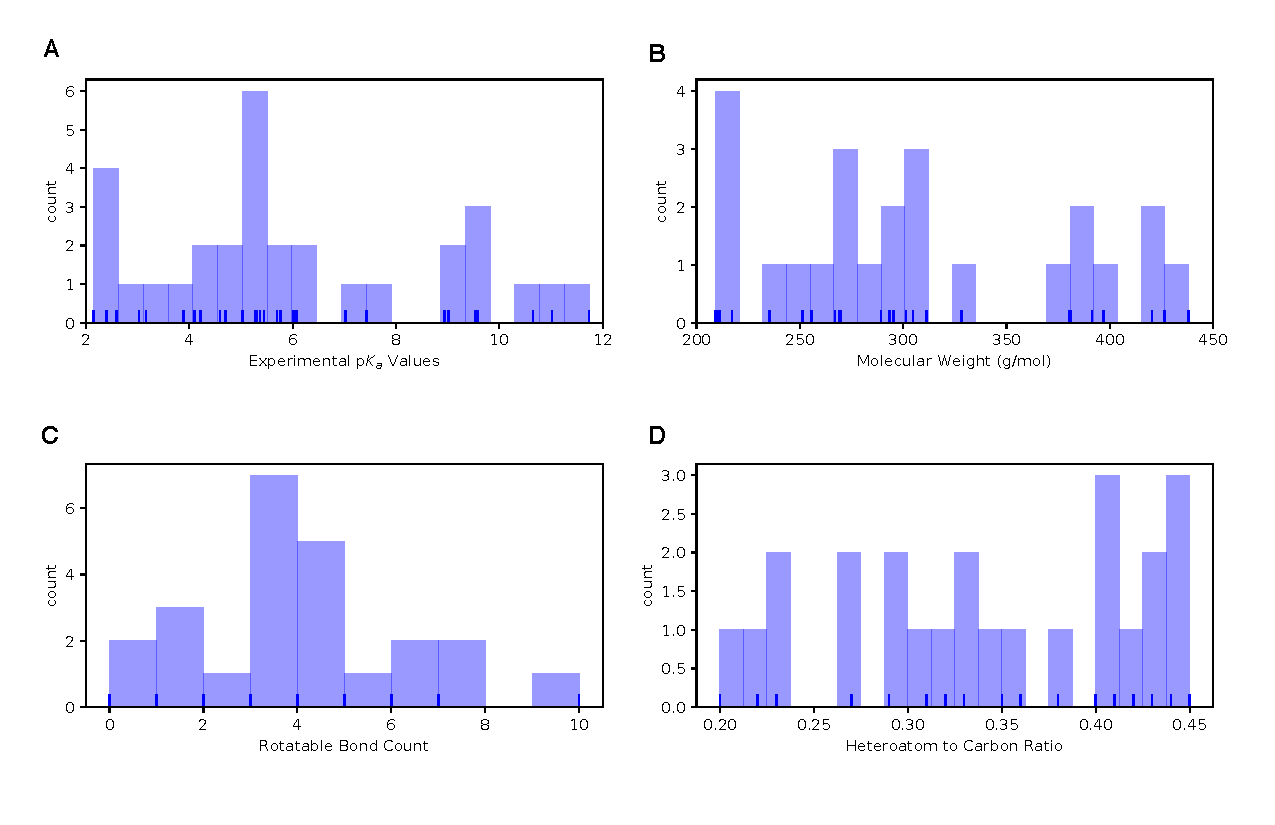
\includegraphics[width=1.0\linewidth]{figures/distribution_of_molecular_properties.pdf}
\caption{{\bf Distribution of molecular properties of the 24 compounds from the SAMPL6 \pKa{} Challenge.} 
{\bf A} Histogram of spectrophotometric \pKa{} measurements collected with Sirius T3 ~\cite{Isik:2018:J.Comput.AidedMol.Des.}. 
The overlaid rug plot indicates the actual values. 
Five compounds have multiple measured \pKa{}s in the range of 2--12. 
{\bf B} Histogram of molecular weights calculated for the neutral state of the compounds in SAMPL6 set. 
Molecular weights were calculated by neglecting counterions.  
{\bf C} Histogram of the number of non-terminal rotatable bonds in each molecule. 
{\bf D} The histogram of the ratio of heteroatom (non-carbon heavy atoms including, O, N, F, S, Cl, Br, I) count to the number of carbon atoms.
}
\label{fig:dist_mol_prop}
\end{center}
\end{figure}

The SAMPL6 \pKa{} Challenge was conducted as a blind prediction challenge and focused on predicting aqueous \pKa{} values of 24 small molecules not previously reported in the literature. 
The challenge set was composed of molecules that resemble fragments of kinase inhibitors. 
Heterocycles that are frequently found in FDA-approved kinase inhibitors were represented in this set. 
The compound selection process was described in depth in the prior publication reporting SAMPL6 \pKa{} Challenge experimental data collection~\citep{Isik:2018:J.Comput.AidedMol.Des.}.
The distribution of molecular weights, experimental \pKa{} values, number of rotatable bonds, and heteroatom to carbon ratio are depicted in Fig.~\ref{fig:dist_mol_prop}. 
The challenge molecule set was composed of 17 small molecules with limited flexibility (less than 5 non-terminal rotatable bonds) and 7 molecules with 5--10 non-terminal rotatable bonds. 
The distribution of experimental \pKa{} values was roughly uniform between 2--12.
2D representations of all compounds are provided in Fig.~\ref{fig:molecules_with_MAE_of_all_methods}. 
Drug-like molecules are often larger and more complex than the ones used in this study. 
We limited the size and the number of rotatable bonds of compounds to create molecule set of intermediate difficulty.

\begin{figure}
\begin{center}
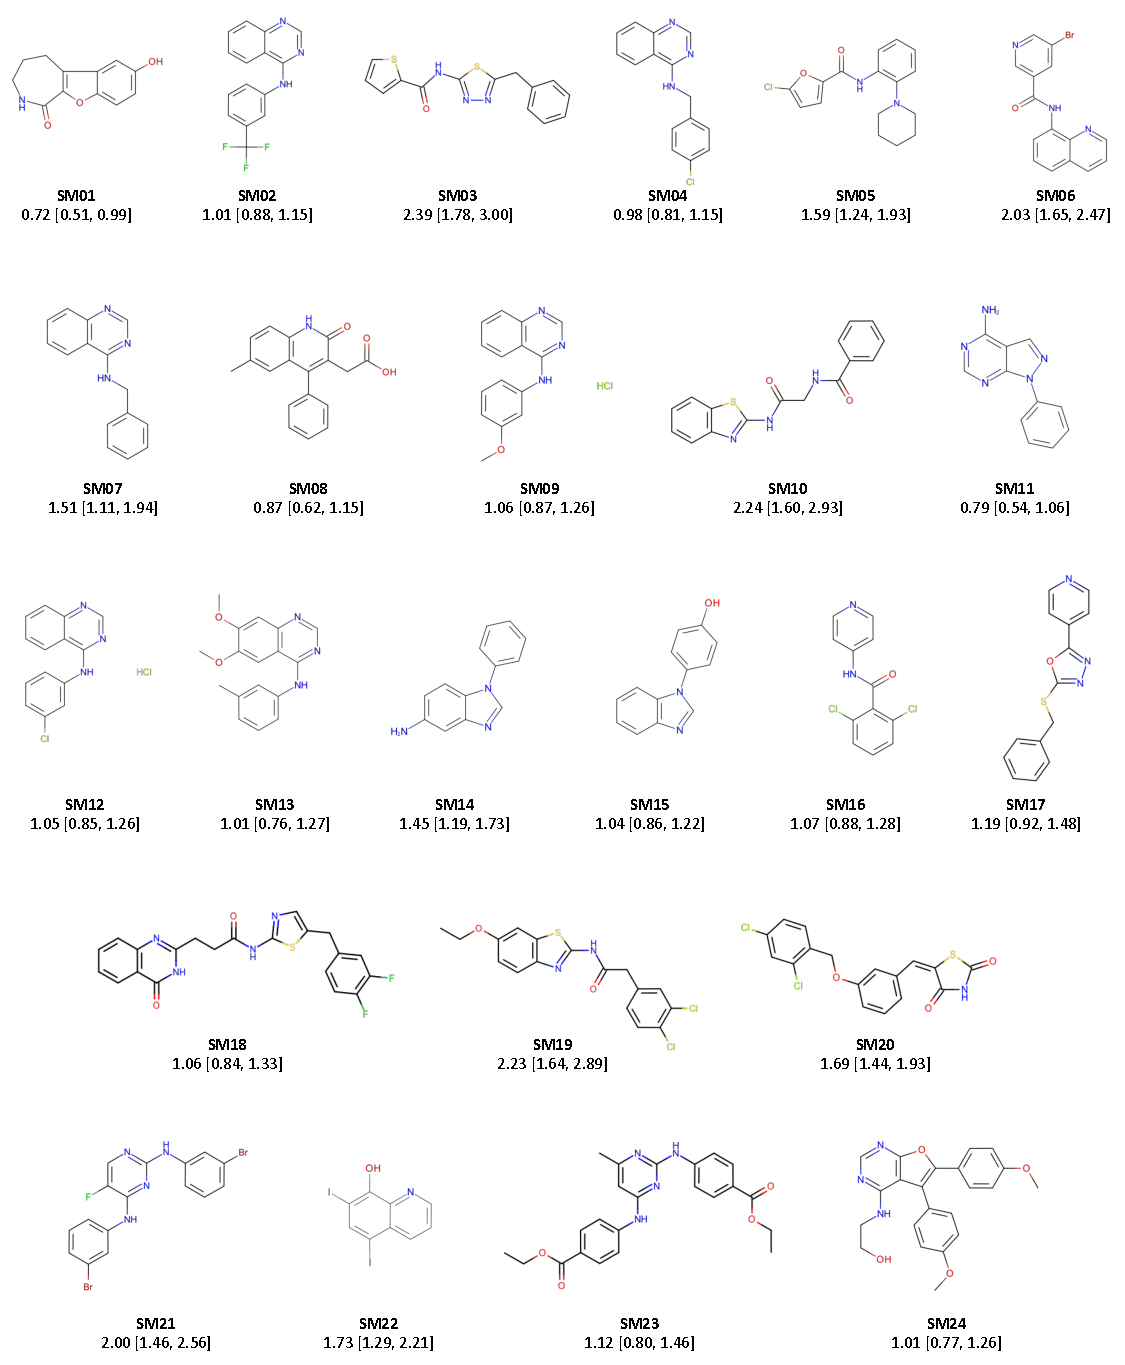
\includegraphics[width=0.95\linewidth]{figures/molecules_with_MAE_of_all_methods.pdf}
\caption{{\bf Molecules from the SAMPL6 Challenge with MAE calculated for all macroscopic \pKa{} predictions.} 
The MAE calculated over all prediction methods indicates which molecules had the lowest prediction accuracy in the SAMPL6 Challenge. 
MAE values calculated for each molecule include all the matched \pKa{} values. 
SM06, SM14, SM15, SM16, SM18, and SM22 were multiprotic. 
Hungarian matching algorithm was employed for pairing experimental and predicted \pKa{} values. 
MAE values are reported with 95\% confidence intervals.
}
\label{fig:molecules_with_MAE_of_all_methods}
\end{center}
\end{figure}

The dataset composition and experimental details---without the identity of the small molecules---were announced approximately one month before the challenge start date. 
Experimental macroscopic \pKa{} measurements were collected using a spectrophotometric method with the Sirius T3 (Sirius Analytical), at room temperature, in ionic strength-adjusted water with 0.15~M KCl~\citep{Isik:2018:J.Comput.AidedMol.Des.}. 
The instructions for participation and the identity of the challenge molecules were released on the challenge start date (October 25, 2017). 
A table of molecule IDs (in the form of SM\#\#) and	their canonical isomeric SMILES was provided as input.
Blind prediction submissions were accepted until January 22, 2018. 

Following the conclusion of the blind challenge, the experimental data was made public on January 23, 2018. 
The SAMPL organizers and participants gathered at the Second Joint D3R/SAMPL Workshop at UC San Diego, La Jolla, CA on February 22--23, 2018 to share results.
The workshop aimed to create an opportunity for participants to discuss the results, evaluate methodological choices by comparing the performance of different methods, and share lessons learned from  the challenge. 
Participants reported their results and their own evaluations in a special issue of the Journal of Computer-Aided Molecular Design~\citep{JCAMD_special_issue_pKa}. 

While designing this first \pKa{} prediction challenge, we did not know the optimal format to capture \pKa{} predictions of participants. 
We wanted to capture all necessary information that will aid the evaluation of \pKa{} predictions at the submission stage. 
Our strategy was to directly evaluate macroscopic \pKa{} predictions comparing them to experimental macroscopic \pKa{} values and to use collected microscopic \pKa{} prediction data for more in-depth diagnostics of method performance.
Therefore, we asked participants to submit their predictions in three different submission types: 
\begin{itemize}
\item {\bf Type I:} microscopic \pKa{} values and related microstate pairs
\item {\bf Type II:} fractional microstate populations as a function of pH in 0.1 pH increments
\item {\bf Type III:} macroscopic \pKa{} values
\end{itemize}

For each submission type, a machine-readable submission file template was specified. 
For type I submissions, participants were asked to report the microstate ID of the protonated state, the microstate ID of deprotonated state, the microscopic \pKa{}, and the predicted microscopic \pKa{} standard error of the mean (SEM).  
The method of microstate enumeration and why it was needed are discussed further in Section~\ref{section-enumeration-of-microstates} "Enumeration of Microstates".
The SEM aims to capture the statistical uncertainty of the prediction method. 
Microstate IDs were preassigned identifiers for each microstate in the form of SM\#\#\_micro\#\#\#. 
For type II submissions, the submission format included a table that started with a microstate ID column and a set of columns reporting the natural logarithm of fractional microstate population values of each predicted microstate for 0.1 pH increments between pH 2 and 12.
For type III submissions participants were asked to report molecule ID, macroscopic \pKa{}, and macroscopic \pKa{} SEM.  

We required participants to submit predictions for all fields for each prediction, but it was not mandatory to submit predictions for all the molecules or all three submission types. 
Although we accepted submissions with partial sets of molecules, it would have been a better choice to require predictions for all the molecules for a better comparison of overall method performance. 
The submission files also included fields for naming the method, listing the software utilized, and a free text section to describe the methodology used in detail. 

Participants were allowed to submit predictions for multiple methods as long as they created separate submission files. 
While anonymous participation was allowed, all participants opted to make their submissions public.
Blind submissions were assigned a unique 5-digit alphanumeric submission ID, which will be used throughout this paper. 
Unique IDs were also assigned when multiple submissions exist for different submissions types of the same method such as microscopic \pKa{} (type I) and macroscopic \pKa{} (type III). 
These submission IDs were also reported in the evaluation papers of participants to allow cross-referencing. 
Submission IDs, participant-provided method names, and method categories are presented in Table~\ref{submission-ID-table}. 
In many cases, multiple types of submissions (type I, II, and III) of the same method were provided by participants as challenge instructions requested. 
Although each prediction set was assigned a separate submission ID, we matched the submissions that originated from the same method according to the reports of the participants for cases where multiple sets of predictions came from a given method.
Submission IDs for both macroscopic (type III) and microscopic (type I) \pKa{} predictions for each method are shown in Table~\ref{submission-ID-table}. 

%%%
\subsection{Enumeration of microstates} \label{section-enumeration-of-microstates}

To capture both the \pKa{} value and titrating proton position for microscopic \pKa{} predictions, we needed microscopic \pKa{} values to be reported together with a pair of microstates which describe the protonated and deprotonated states corresponding to each microscopic transition.
String representations of molecules such as canonical SMILES with explicit hydrogens can be written, however, there can be inconsistencies between the interpretation of canonical SMILES written by different software and algorithms. 
To avoid complications while reading microstate structure files from different sources, we decided that the safest route was pre-enumerating all possible microstates of challenge compounds, assigning microstate IDs to each in the form of SM\#\#\_micro\#\#\#, and requiring participants to report microscopic \pKa{} values along with microstate pairs specified by the provided microstates IDs.   

We created initial sets of microstates with Schrödinger Epik~\citep{Shelley:2007:J.Comput.AidedMol.Des.} and OpenEye QUACPAC~\citep{quacpac_openeye_2017} and took the union of results. 
Microstates with Epik were generated using Schr\"{o}dinger Suite v2016-4, running Epik to enumerate all tautomers within 20 \pKa{} units of pH 7.
For enumerating microstates with OpenEye QUACPAC, we had to first enumerate formal charges and for each charge enumerate all possible tautomers using the settings of maximum tautomer count 200, level 5, with carbonyl hybridization set to False.
Then we created a union of all enumerated states written as canonical isomeric SMILES generated by OpenEye OEChem~\citep{oechem_openeye_2017}.
Even though resonance structures correspond to different canonical isomeric SMILES, they are not different microstates, therefore it was necessary to remove resonance structures that were replicates of the same tautomer. 
To detect equivalent resonance structures, we converted canonical isomeric SMILES to InChI hashes with explicit and fixed hydrogen layer. 
Structures that describe the same tautomer but different resonance states lead to explicit hydrogen InChI hashes that are identical, allowing replicates to be removed. 
The Jupyter Notebook used for the enumeration of microstates is provided in Supplementary Information. 

We provided microstate ID tables with canonical SMILES and 2D depictions to aid participants in matching predicted structures to microstate IDs. 
A canonical SMILES representation was selected over canonical isomeric SMILES, because resonance and geometric isomerism do not lead to different microstates according to our working microstate definition. 
The only exception was for molecule SM20, which should be consistently modeled as the E-isomer.

During the course of the SAMPL6 Challenge, participants identified new microstates that were not present in the initial list that we provided. 
Despite combining enumerated charge states and tautomers generated by both Epik and OpenEye QUACPAC, to our surprise, the microstate lists were still incomplete.
Based on participant requests for new microstates, we iteratively had to update the list of microstates and assign new microstate IDs.
Every time we received a request, we shared the updated microstate ID lists with all challenge participants.
Some participants updated their \pKa{} prediction by including the newly added microstates in their calculations. 
In the future, developing a better algorithm that can enumerate all possible microstates (not just the ones with significant populations) would be very beneficial for anticipating microstates that may be predicted by \pKa{} prediction methods. 


A microscopic \pKa{} definition was provided in challenge instructions for clarity as follows:
Physically meaningful microscopic \pKa{}s are defined between microstate pairs that can interconvert by single protonation/deprotonation event of only one titrable group. 
So, microstate pairs should have total charge (absolute) difference of 1 and only one heavy atom that differs in the number of associated hydrogens, regardless of resonance state or geometric isomerism. 
All geometric isomer and resonance structure pairs that have the same number of hydrogens bound to equivalent heavy atoms are grouped into the same microstate. 
Pairs of resonance structures and geometric isomers (cis/trans, stereo) are not considered as different microstates, as long as there is no change in the number of hydrogens bound to each heavy atom.
Transitions where there are shifts in the position of protons coupled to changes in the number of protons were also not considered as microscopic \pKa{}~ values~\citep{Gunner:2020:J.Comput.AidedMol.Des.}.
Since we wanted participants to report only microscopic \pKa{}s that describe single deprotonation events (in contrast to transitions between microstates that are different in terms of two or more titratable protons), we have also provided a pre-enumerated list of allowed microstate pairs.


Provided microstate ID and microstate pair lists were intended to be used for reporting microstate IDs and to aid parsing of submissions. 
The enumerated lists of microstates were not created with the intent to guide computational predictions. 
This was clearly stated in the challenge instructions. 
However, we noticed that some participants still used the microstate lists as an input for their \pKa{} predictions as we received complaints from participants that due to our updates to microstate lists they needed to repeat their calculations. 
This would not have been an issue if participants used \pKa{} prediction protocols that did not rely on an external pre-enumerated list of microstates as an input.
None of the participants reported this dependency in their method descriptions explicitly, so it was also not obvious how participants were using the provided states in their predictions.
We could not identify which submissions used these enumerated microstate lists as input for predictions and which have followed the challenge instructions and relied only on their prediction method to generate microstates.

%%%
\subsection{Evaluation approaches}

Since the experimental data for the challenge was mainly composed of macroscopic \pKa{} values of both monoprotic and multiprotic compounds, evaluation of macroscopic and microscopic \pKa{} predictions was not straightforward. 
For a subset of 8 molecules, the dominant microstate sequence could be inferred from NMR experiments. 
For the rest of the molecules, the only experimental information available was the macroscopic \pKa{} value.
The experimental data---in the form of macroscopic \pKa{}~ values---did not provide any information on which group(s) are being titrated, the microscopic \pKa{} values, the identity of the associated macrostates (which total charge), or microstates (which tautomers). 
Also, experimental data did not provide any information about the charge state of protonated and deprotonated species associated with each macroscopic \pKa{}. 
Typically charges of states associated with experimental \pKa{} values are assigned based on \pKa{} predictions, not experimental evidence, but we did not utilize such computational charge assignment.
For a fair performance comparison between methods, we avoided relying on any particular \pKa{} prediction to assist the interpretation of the experimental reference data.
This choice complicated the \pKa{} prediction analysis, especially regarding how to pair experimental and predicted \pKa{}~ values for error analysis.
We adopted various evaluation strategies guided by the experimental data. 
To compare macroscopic \pKa{} predictions to experimental values, we had to utilize numerical matching algorithms before we could calculate performance statistics. 
For the subset of molecules with experimental data about microstates, we used microstate-based matching. 
These matching methods are described in more detail in the next section.

Three types of submissions were collected during the SAMPL6 \pKa{} Challenge. 
We have only utilized the type I (microscopic \pKa{} value and microstate IDs) and the type III (macroscopic \pKa{} value) predictions in this article. 
Type I submissions contained the same prediction information as the type II submissions which reported the fractional population of microstates with respect to pH.
We collected type II submissions in order to capture relative populations of microstates, not realizing they were redundant.  
The microscopic \pKa{} predictions collected in type I submissions capture all the information necessary to calculate type II submissions. 
Therefore, we did not use type II submissions for challenge evaluation. 
In theory, type III (macroscopic \pKa{}) predictions can also be calculated from type I submissions, but collecting type III submissions allowed the participation of \pKa{} prediction methods that directly predict macroscopic \pKa{}~ values without considering microspeciation and methods that apply special empirical corrections for macroscopic \pKa{} predictions.

\subsubsection{Matching algorithms for pairing predicted and experimental \pKa{}~ values}

Macroscopic \pKa{} predictions can be calculated from microscopic \pKa{}~ values for direct comparison to experimental macroscopic \pKa{} values.
One major question must be answered to allow this comparison:  
How should we match predicted macroscopic \pKa{}~ values to experimental macroscopic \pKa{}~ values when there could multiple \pKa{} values reported for a given molecule?
For example, experiments on SM18 showed three macroscopic \pKa{}s, but prediction of \textit{xvxzd} method reported two macroscopic \pKa{} values. 
% SM18 experimental pKa: 2.15 $\pm$ 0.02, 9.58 $\pm$  0.03, and 11.02 $\pm$ 0.04 % % SM18 predicted \pKa{} (xvxzd) values for this molecule by were 2.15 $\pm$ 0.23 and 8.52 $\pm$ 0.33
There were also examples of the opposite situation with more predicted \pKa{} values than experimentally determined macroscopic \pKa{}s: One experimental \pKa{} was measured for SM02, but two macroscopic \pKa{}~ values were predicted by \textit{xvxzd} method.
% SM02 exp: 5.03
%SM02 pred: 4.93 11.44
The experimental and predicted values must be paired before any prediction error can be calculated, even though there was not any experimental information regarding underlying tautomer and charge states. 

Knowing the charges of macrostates would have guided the pairing between experimental and predicted macroscopic \pKa{}~ values, however, not all experimental \pKa{} measurements can determine determine the charge of protonation states. 
The potentiometric \pKa{} measurements just captures the relative charge change between macrostates, but not the absolute value of the charge.  
Thus, our experimental data did not provide any information that would indicate the titration site, the overall charge, or the tautomer composition of macrostate pairs that are associated with each measured macroscopic \pKa{} that can guide the matching between predicted and experimental \pKa{} values. 
 

For evaluating macroscopic \pKa{} predictions taking the experimental data as reference, Fraczkiewicz \citep{Fraczkiewicz:2013:ReferenceModuleinChemistryMolecularSciencesandChemicalEngineering} delineated recommendations for fair comparative analysis of computational \pKa{} predictions. 
They recommended that, in the absence of any experimental information that would aid in matching, experimental and computational \pKa{}~ values should be matched preserving the order of \pKa{} values and minimizing the sum of absolute errors.

We picked the Hungarian matching algorithm~\citep{Kuhn:1955:Nav.Res.Logist.Q., Munkres:1957:JSIAM} to match experimental and predicted macroscopic \pKa{}~ values with a squared error cost function as suggested by Kiril Lanevskij via personal communication. 
The algorithm is available in the SciPy package (\textit{scipy.optimize.linear\_sum\_assignment})~\citep{SciPy-linear-sum-assignment}.
This matching algorithm provides optimum global assignment that minimizes the linear sum of squared errors of all pairwise matches.
We selected the squared error cost function instead of the absolute error cost function to avoid misordered matches,
For instance, for a molecule with experimental \pKa{} values of 4 and 6, and predicted \pKa{}~ values of 7 and 8, Hungarian matching with absolute error cost function would match 6 to 7 and 4 to 9.
Hungarian matching with squared error cost would match 4 to 7 and 6 to 9, preserving the increasing \pKa{} value order between experimental and predicted values.
A weakness of this approach would be failing to match the experimental value of 6 to predicted value of 7 if that was the correct match based on underlying macrostates. 
But the underlying pair of states were unknown to us both because the experimental data did not determine which charge states the transitions were happening between and also because we did not collect the pair of macrostates associated with each \pKa{} predictions in submissions. 
Requiring this information for macroscopic \pKa{} predictions in future SAMPL challenges would allow for better comparison between predictions, even if experimental assignment of charges is not possible.
There is no perfect solution to the numerical \pKa{} assignment problem, but we tried to determine the fairest way to penalize predictions based on their numerical deviation from the experimental values.

For the analysis of microscopic \pKa{} predictions we adopted a different matching approach. 
For the eight molecules for which we had the requisite data for this analysis, we utilized the dominant microstate sequence inferred from NMR experiments to match computational predictions and experimental \pKa{}~ values. 
We will refer to this assignment method as microstate matching, where the experimental \pKa{} value is matched to the computational microscopic \pKa{} value which was reported for the dominant microstate pair observed for each transition. 
We have compared the results of Hungarian matching and microstate matching. 

Inevitably, the choice of matching algorithms to assign experimental and predicted values has an impact on the computed performance statistics. 
We believe the Hungarian algorithm for numerical matching of unassigned \pKa{} values and microstate-based matching when experimental microstates are known were the best choices, providing the most unbiased matching without introducing assumptions outside of the experimental data.


\subsubsection{Statistical metrics for submission performance}

A variety of accuracy and correlation statistics were considered for analyzing and comparing the performance of prediction methods submitted to the SAMPL6 \pKa{} Challenge. 
Calculated performance statistics of predictions were provided to participants before the workshop. 
Details of the analysis and scripts are maintained on the SAMPL6 GitHub Repository (described in Section~\ref{Code-and-Data-Availability}).

\paragraph{Error metrics}

There are six error metrics reported for the numerical error of the \pKa{} values: the root-mean-squared error (RMSE), mean absolute error (MAE), mean error (ME), coefficient of determination (R\textsuperscript{2}), linear regression slope (m), and Kendall’s Rank Correlation Coefficient ($\tau$).
Uncertainty in each performance statistic was calculated as 95\% confidence intervals estimated by non-parametric bootstrapping (sampling with replacement) over predictions with 10~000 bootstrap samples. 
Calculated errors statistics of all methods can be found in Table~\ref{SI_statistics_table_macro_pKa} for macroscopic \pKa{} predictions and Tables~\ref{SI-statistics-table-micro-pKa-8mol-microstate} and \ref{SI-statistics-table-micro-pKa-8mol-microstate} for microscopic \pKa{} predictions. 

\paragraph{Assessing macrostate predictions}

In addition to assessing the numerical error in predicted \pKa{} values, we also evaluated predictions in terms of their ability to capture the correct macrostates (ionization states) and microstates (tautomers of each ionization state) to the extent possible from the available experimental data. 
For macroscopic \pKa{}s, the spectrophotometric experiments do not directly report on the identity of the ionization states. 
However, the number of ionization states indicates the number of macroscopic \pKa{}s that exists between the experimental range of 2.0--12.0. 
For instance, SM14 has two experimental \pKa{}s and therefore three different charge states observed between pH 2.0 and 12.0. 
If a prediction reported 4 macroscopic \pKa{}s, it is clear that this method predicted an extra ionization state. 
With this perspective, we reported the number of unmatched experimental \pKa{}s (the number of missing \pKa{} predictions, i.e., missing ionization states) and the number of unmatched predicted \pKa{}s (the number of extra \pKa{} predictions, i.e., extra ionization states) after Hungarian matching. 
The latter count was restricted to only predictions with \pKa{} values between 2 and 12 because that was the range of the experimental method. 
Errors in extra or missing \pKa{} prediction errors highlight failure to predict the correct number of ionization states within a pH range.


\paragraph{Assessing microstate predictions}

For the evaluation of microscopic \pKa{} predictions, taking advantage of the available dominant microstate sequence data for a subset of 8 compounds, we calculated the dominant microstate prediction accuracy which is the ratio of correct dominant tautomer predictions for each charge state divided by the total number of dominant tautomer predictions. 
Dominant microstate prediction accuracy was calculated over all experimentally detected ionization states of each molecule which were part of this analysis. 
In order to extract the sequence of dominant microstates from the microscopic \pKa{} predictions sets, we calculated the relative free energy of microstates selecting a neutral tautomer and pH 0 as reference following Equation~\ref{eq:microstate_relative_free_energy}. 
Calculation of relative microstate free energies was explained in more detail in a previous publication~\citep{Gunner:2020:J.Comput.AidedMol.Des.}. 

The relative free energy of a state with respect to reference state B at pH 0.0 (arbitrary pH value selected as reference) can be calculated as follows: 
\begin{equation}
\Delta G_{AB} = \Delta m_{AB} \:RT\ln{10}\:(pH - pK_{a})
\label{eq:microstate_relative_free_energy}
\end{equation}
$\Delta m_{AB}$ is equal to the number protons in state A minus that in state B. R and T indicate the molar gas constant and temperature, respectively. 
By calculating relative free energies of all predicted microstates with respect to the same reference state and pH, we were able to determine the sequence of predicted dominant microstates. 
The dominant tautomer of each charge state was determined as the microstate with the lowest free energy in the subset of predicted microstates of each ionization state. 
This approach is feasible because the relative free energy of tautomers of the same ionization state is independent of pH and therefore the choice of reference pH is arbitrary.

\paragraph{Identifying consistently top-performing methods}

We created a shortlist of top-performing methods for macroscopic and microscopic \pKa{} predictions. 
The top macroscopic \pKa{} predictions were selected if they ranked in the top 10 consistently according to two error metrics (RMSE, MAE) and two correlation metrics (R-Squared, and Kendall’s Tau), while also having fewer than eight missing or extra macroscopic \pKa{}s for the entire molecule set (eight macrostate errors correspond to macrostate prediction mistake in roughly one third of the 24 compounds). 
These methods are presented in Table~\ref{typeIII-well-performing-methods-table}. A separate list of top-performing methods was constructed for microscopic \pKa{} with the following criteria: ranking in the top 10 methods when ranked by accuracy statistics (RMSE and MAE) and perfect dominant microstate prediction accuracy. 
These methods are presented in Table~\ref{typeI-well-performing-methods-table}.

\paragraph{Determining challenging molecules}

In addition to comparing the performance of methods, we also wanted to compare \pKa{} prediction performance for each molecule to determine which molecules were the most challenging for \pKa{} predictions considering all the methods in the challenge. 
For this purpose, we plotted prediction error distributions of each molecule calculated over all prediction methods. 
We also calculated MAE for each molecule over all prediction sets as well as for predictions from each method category separately. 


%%%
\subsection{Reference calculations}

Including a null model is helpful in comparative performance analysis of predictive methods to establish what the performance statistics look like for a baseline method for the specific dataset. 
Null models or null predictions employ a simple prediction model which is not expected to be particularly successful, but it provides a simple point of comparison for more sophisticated methods. 
The expectation or goal is for more sophisticated or costly prediction methods to outperform the predictions from a null model, otherwise the simpler null model would be preferable. 
In SAMPL6 \pKa{} Challenge there were two blind submissions using database lookup methods that were submitted to serve as null predictions. These methods, with submission IDs \textit{5nm4j} and \textit{5nm4j} both used OpenEye pKa-Prospector database to find the most similar molecule to query molecule and simply reported its \pKa{} as the predicted value. 
Database lookup methods with a rich experimental database do present a challenging null model to beat, however, due to the accuracy level needed from \pKa{} predictions for computer-aided drug design we believe such methods provide an appropriate performance baseline that physical and empirical \pKa{} prediction methods should strive to outperform.

We also included additional reference calculations in the comparative analysis to provide more perspective. 
Some widely used methods by academia and industry were missing from the blind challenge submission. Therefore, we included those methods as reference calculations: Schr\"{o}dinger/Epik (\textit{nb007, nb008, nb010}), Schr\"{o}dinger/Jaguar (\textit{nb011, nb013}), Chemaxon/Chemicalize (\textit{nb015}), and Molecular Discovery/MoKa (\textit{nb016, nb017}). 
Epik and Jaguar \pKa{} predictions were collected by Bas Rustenburg, Chemicalize predictions by Mehtap Isik, and MoKa predictions by Thomas Fox. 
All were done after the challenge deadline avoiding any alterations to their respective standard procedures and any guidance from experimental data. 
Experimental data was publicly available before these calculations were complete, therefore reference calculations were not formally considered as blind submissions. 

All figures and statistics tables in this manuscript include reference calculations. 
As the reference calculations were not formal submissions, these were omitted from formal ranking in the challenge, but we present plots in this article which show them for easy comparison. 
These are labeled with submission IDs of the form \textit{nb\#\#\#} to clearly indicate non-blind reference calculations.


%%%%%%%%%%%%%%%%%%%%%%%%%%%%%%%%%%%%%%%%%%%%%%%%%%%%%%%%%%%%
% Results and Discussion
%%%%%%%%%%%%%%%%%%%%%%%%%%%%%%%%%%%%%%%%%%%%%%%%%%%%%%%%%%%%
\section{Results and Discussion}


Participation in the SAMPL6 \pKa{} Challenge was high with 11 research groups contributing \pKa{} prediction sets for 37 methods.  
A large variety of \pKa{} prediction methods were represented in the SAMPL6 Challenge. 
We categorized these submissions into four method classes: database lookup (DL), linear free energy relationship (LFER), quantitative structure-property relationship or machine learning (QSPR/ML), and quantum mechanics (QM). 
Quantum mechanics models were subcategorized into QM methods with and without linear empirical correction (LEC), and combined quantum mechanics and molecular mechanics (QM + MM). 
Table~\ref{submission-ID-table} presents method names, submission IDs, method categories, and also references for each approach. 
Integral equation-based approaches (e.g.EC-RISM) were also evaluated under the Physical (QM) category. 
There were 2 DL, 4 LFER, and 5 QSPR/ML methods represented in the challenge, including the reference calculations. 
The majority of QM calculations include linear empirical corrections (22 methods in QM + LEC category), and only 5 QM methods were submitted without any empirical corrections. 
There were 4 methods that used a mixed physical modeling approach of QM + MM. 

The following sections present a detailed performance evaluation of blind submissions and reference prediction methods for macroscopic and microscopic \pKa{} predictions. 
Performance statistics of all the methods can be found in Tables~\ref{SI_statistics_table_macro_pKa} and \ref{SI-statistics-table-micro-pKa-8mol-microstate}. 
Methods are referred to by their submission ID's which are provided in Table \ref{submission-ID-table}.



\begin{table}%[H]%[tb!]
\begin{center}
\begin{threeparttable}
\centering\scriptsize
\caption{{\bf Submission IDs, names, category, and type for all the \pKa{} prediction sets.}
Reference calculations are labeled as \textit{nb\#\#\#}. 
The method name column lists the names provided by each participant in the submission file. 
The ``type'' column indicates if a submission was or a post-deadline reference calculation, denoted by ``Blind'' or ``Reference'' respectively. 
The methods in the table are grouped by method category and not ordered by performance.  
} 
\label{submission-ID-table}
\begin{tabular}{llllll}
\hline
\textbf{\begin{tabular}[c]{@{}l@{}}Method \\ Category\end{tabular}} & \textbf{Method} & \textbf{\begin{tabular}[c]{@{}l@{}}Microscopic \pKa{} \\ (Type I) \\ Submission ID\end{tabular}} & \textbf{\begin{tabular}[c]{@{}l@{}}Macroscopic \pKa{} \\ (Type III) \\ Submission ID\end{tabular}} & \textbf{\begin{tabular}[c]{@{}l@{}}Submission \\ Type\end{tabular}} & \textbf{Ref.} \\ \hline
\rowcolor[HTML]{EFEFEF} 
DL & Substructure matches to experimental data in pKa OpenEye pKa Prospector Database v1.0 & \textit{} & \textit{5nm4j} & Null & \cite{pKa-prospector-ref} \\
DL & OpenEye pKa-Prospector 1.0.0.3 with Analog Search ion identification algorithm & \textit{} & \textit{pwn3m} & Null & \cite{pKa-prospector-ref} \\
\rowcolor[HTML]{EFEFEF} 
LFER & ACD/pKa GALAS (ACD/Percepta Kernel v1.6) & \textit{v8qph} & \textit{37xm8} & Blind & \cite{ACD-pKa-galas} \\
LFER & ACD/pKa Classic (ACD/Percepta Kernel, v1.6) & \textit{} & \textit{xmyhm} & Blind & \cite{ACD-pKa-classic} \\
\rowcolor[HTML]{EFEFEF} 
LFER & Epik Scan (Schr\"{o}dinger v2017-4) & \textit{} & \textit{nb007} & Reference & \cite{Shelley:2007:J.Comput.AidedMol.Des.} \\
LFER & Epik Microscopic (Schr\"{o}dinger v2017-4) & \textit{nb008} & \textit{nb010} & Reference & \cite{Shelley:2007:J.Comput.AidedMol.Des.} \\
\rowcolor[HTML]{EFEFEF} 
QSPR/ML & OpenEye Gaussian Process & \textit{6tvf8} & \textit{hytjn} & Blind & \cite{Bannan:2018:J.Comput.AidedMol.Des.} \\
QSPR/ML & OpenEye Gaussian Process Resampled & \textit{} & \textit{q3pfp} & Blind & \cite{Bannan:2018:J.Comput.AidedMol.Des.} \\
\rowcolor[HTML]{EFEFEF} 
QSPR/ML & S+pKa (ADMET Predictor v8.5, Simulations Plus) & \textit{hdiyq} & \textit{gyuhx} & Blind & \cite{simulation-plus-pKa} \\
QSPR/ML & Chemicalize v18.23 (ChemAxon MarvinSketch v18.23) & \textit{} & \textit{nb015} & Reference & \cite{chemicalize-pKa} \\
\rowcolor[HTML]{EFEFEF} 
QSPR/ML & MoKa v3.1.3 & \textit{nb016} & \textit{nb017} & Reference & \cite{Milletti:2007:J.Chem.Inf.Model., moka-pKa} \\
\rowcolor[HTML]{EFEFEF} 
QM & \begin{tabular}[c]{@{}l@{}}Adiabatic scheme with single point correction:  SMD/M06-2X//6-311++G(d,p)//M06-2X/6-31+G(d) \\ for bases and SMD/M06-2X//6-311++G(d,p)//M06-2X/6-31G(d) for acids  + thermal corrections\end{tabular} & \textit{ko8yx} & \textit{ryzue} & Blind & \cite{Zeng:2018:J.Comput.AidedMol.Des.} \\
QM & \begin{tabular}[c]{@{}l@{}}Direct scheme with single point correction: SMD/M06-2X//6-311++G(d,p)//M06-2X/6-31+G(d) for \\ bases and SMD/M06-2X//6-311++G(d,p)//M06-2X/6-31G(d) for acids  + thermal corrections\end{tabular} & \textit{w4z0e} & \textit{xikp8} & Blind & \cite{Zeng:2018:J.Comput.AidedMol.Des.} \\
\rowcolor[HTML]{EFEFEF} 
QM & \begin{tabular}[c]{@{}l@{}}Adiabatic scheme: thermodynamic cycle that uses gas phase optimized structures for gas phase free \\ energy and solution phase geometries for solvent phase free energy. SMD/M06-2X/6-31+G(d) for \\ bases and SMD/M06-2X/6-31G(d) for acids + thermal corrections\end{tabular} & \textit{wcvnu} & \textit{5byn6} & Blind & \cite{Zeng:2018:J.Comput.AidedMol.Des.} \\
QM & \begin{tabular}[c]{@{}l@{}}Vertical scheme:  thermodynamic cycle that uses only gas phase optimized structures to compute gas \\ hase and solvation free energy. SMD/M06-2X/6-31+G(d) for bases and SMD/M06-2X/6-31G(d) for \\ acids + Thermal corrections\end{tabular} & \textit{arcko} & \textit{w4iyd} & Blind & \cite{Zeng:2018:J.Comput.AidedMol.Des.} \\
\rowcolor[HTML]{EFEFEF} 
QM & \begin{tabular}[c]{@{}l@{}}Direct scheme: solution phase free energy is determined by solution phase geometries  without \\ thermodynamic cycle SMD/M06-2X/6-31+G(d) for bases and SMD/M06-2X/6-31G(d) for acids \\ + thermal corrections\end{tabular} & \textit{wexjs} & \textit{y75vj} & Blind & \cite{Zeng:2018:J.Comput.AidedMol.Des.} \\
QM + LEC & Jaguar (Schr\"{o}dinger v2017-4) & \textit{nb011} & \textit{nb013} & Reference & \cite{Bochevarov:2013:Int.J.QuantumChem.} \\
\rowcolor[HTML]{EFEFEF} 
QM + LEC & CPCM/B3LYP/6–311+G(d,p) and global fitting & \textit{y4wws} & \textit{35bdm} & Blind & \cite{Selwa:2018:J.Comput.AidedMol.Des.} \\
QM + LEC & \begin{tabular}[c]{@{}l@{}}CPCM/B3LYP/6–311+G(d,p) and separate fitting for neutral to negative and for positive to neutral \\ transformations\end{tabular} & \textit{qsicn} & \textit{p0jba} & Blind & \cite{Selwa:2018:J.Comput.AidedMol.Des.} \\
\rowcolor[HTML]{EFEFEF} 
QM + LEC & EC-RISM/MP2/6-311+G(d,p)-P3NI-q-noThiols-2par & \textit{kxztt} & \textit{ds62k} & Blind & \cite{Tielker:2018:J.Comput.AidedMol.Des.} \\
QM + LEC & EC-RISM/MP2/cc-pVTZ-P2-q-noThiols-2par & \textit{ftc8w} & \textit{2ii2g} & Blind & \cite{Tielker:2018:J.Comput.AidedMol.Des.} \\
\rowcolor[HTML]{EFEFEF} 
QM + LEC & EC-RISM/MP2/6-311+G(d,p)-P2-phi-all-2par & \textit{ktpj5} & \textit{nb001} & Blind* & \cite{Tielker:2018:J.Comput.AidedMol.Des.} \\
QM + LEC & EC-RISM/MP2/6-311+G(d,p)-P2-phi-noThiols-2par & \textit{wuuvc} & \textit{nb002} & Blind* & \cite{Tielker:2018:J.Comput.AidedMol.Des.} \\
\rowcolor[HTML]{EFEFEF} 
QM + LEC & EC-RISM/MP2/6-311+G(d,p)-P3NI-phi-all-2par & \textit{2umai} & \textit{nb003} & Blind* & \cite{Tielker:2018:J.Comput.AidedMol.Des.} \\
QM + LEC & EC-RISM/MP2/6-311+G(d,p)-P3NI-phi-noThiols-2par & \textit{cm2yq} & \textit{nb004} & Blind* & \cite{Tielker:2018:J.Comput.AidedMol.Des.} \\
\rowcolor[HTML]{EFEFEF} 
QM + LEC & EC-RISM/MP2/6-311+G(d,p)-P2-phi-all-1par & \textit{z7fhp} & \textit{nb005} & Blind* & \cite{Tielker:2018:J.Comput.AidedMol.Des.} \\
QM + LEC & EC-RISM/MP2/6-311+G(d,p)-P3NI-phi-all-1par & \textit{8toyp} & \textit{nb006} & Blind* & \cite{Tielker:2018:J.Comput.AidedMol.Des.} \\
\rowcolor[HTML]{EFEFEF} 
QM + LEC & EC-RISM/MP2/cc-pVTZ-P2-phi-noThiols-2par & \textit{epvmk} & \textit{ttjd0} & Blind & \cite{Tielker:2018:J.Comput.AidedMol.Des.} \\
QM + LEC & EC-RISM/MP2/cc-pVTZ-P2-phi-all-2par & \textit{xnoe0} & \textit{mkhqa} & Blind & \cite{Tielker:2018:J.Comput.AidedMol.Des.} \\
\rowcolor[HTML]{EFEFEF} 
QM + LEC & EC-RISM/MP2/cc-pVTZ-P3NI-phi-noThiols-2par & \textit{4o0ia} & \textit{mpwiy} & Blind & \cite{Tielker:2018:J.Comput.AidedMol.Des.} \\
QM + LEC & EC-RISM/B3LYP/6-311+G(d,p)-P3NI-q-noThiols-2par & \textit{nxaaw} & \textit{ad5pu} & Blind & \cite{Tielker:2018:J.Comput.AidedMol.Des.} \\
\rowcolor[HTML]{EFEFEF} 
QM + LEC & EC-RISM/B3LYP/6-311+G(d,p)-P3NI-phi-noThiols-2par & \textit{0xi4b} & \textit{f0gew} & Blind & \cite{Tielker:2018:J.Comput.AidedMol.Des.} \\
QM + LEC & EC-RISM/B3LYP/6-311+G(d,p)-P2-phi-noThiols-2par & \textit{cywyk} & \textit{np6b4} & Blind & \cite{Tielker:2018:J.Comput.AidedMol.Des.} \\
\rowcolor[HTML]{EFEFEF} 
QM + LEC & PCM/B3LYP/6-311+G(d,p) & \textit{gdqeg} & \textit{yc70m} & Blind & \cite{Tielker:2018:J.Comput.AidedMol.Des.} \\
QM + LEC & COSMOtherm\_FINE17 (COSMOtherm C30\_1701, BP/TZVPD/FINE//BP/TZVP/COSMO) & \textit{t8ewk} & \textit{0hxtm} & Blind & \cite{Klamt:2003:J.Phys.Chem.Ab, Eckert:2006:J.Comput.Chem.} \\
\rowcolor[HTML]{EFEFEF} 
QM + LEC & \begin{tabular}[c]{@{}l@{}}DSD-BLYP-D3(BJ)/def2-TZVPD//PBEh-3c[DCOSMO-RS] + RRHO(GFN-xTB[GBSA]) \\ + Gsolv(COSMO-RS[TZVPD]) and linear fit\end{tabular} & \textit{} & \textit{xvxzd} & Blind & \cite{Pracht:2018:J.Comput.AidedMol.Des.} \\
QM + LEC & \begin{tabular}[c]{@{}l@{}}ReSCoSS conformations // DSD-BLYP-D3 reranking // COSMOtherm pKa:  DSD-BLYP-D3(BJ)/\\ def2-TZVPD// PBE-D3(BJ)/def2-TZVP/COSMO + RRHO[GFN-xTB + GBSA-water] \\ + Gsolv[COSMO-RS(FINE17/TZVPD)] level and COSMOtherm pKa applied  at the single conformer \\ pair level  (COSMOthermX17.0.5 release and BP-TZVPD-FINE-C30-1701 parameterization)\end{tabular} & \textit{eyetm} & \textit{8xt50} & Blind & \cite{Pracht:2018:J.Comput.AidedMol.Des.} \\
\rowcolor[HTML]{EFEFEF} 
QM + LEC & \begin{tabular}[c]{@{}l@{}}ReSCoSS conformations // COSMOtherm pKa: DSD-BLYP-D3(BJ)/def2-TZVPD// PBE-D3(BJ)/\\ def2-TZVP/COSMO + RRHO[GFN-xTB + GBSA-water] + Gsolv[COSMO-RS(FINE17/TZVPD)] \\ level and COSMOtherm pKa was applied directly on the resulting conformer sets with at least 5\% \\ Boltzmann weights for each microspecies (COSMOthermX17.0.5 release and BP-TZVPD-FINE-\\ C30-1701 parameterization)\end{tabular} & \textit{ccpmw} & \textit{yqkga} & Blind & \cite{Pracht:2018:J.Comput.AidedMol.Des.} \\
QM + MM & \begin{tabular}[c]{@{}l@{}}M06-2X/6-31G*(for bases) or 6-31+G*(for acids) for gas phase, solvation free energy using TI with \\ explicit solvent and GAFF, solvation free energy of proton -265.6 kcal/mol\end{tabular} & \textit{0wfzo} & \textit{} & Blind & \cite{Prasad:2018:J.Comput.AidedMol.Des.} \\
\rowcolor[HTML]{EFEFEF} 
QM + MM & \begin{tabular}[c]{@{}l@{}}M06-2X/6-31G*(for bases) or 6-31+G*(for acids) for gas phase, solvation free energy using TI with \\ explicit solvent and GAFF, solvation free energy of proton -271.88 kcal/mol\end{tabular} & \textit{z3btx} & \textit{} & Blind &  \\
QM + MM & \begin{tabular}[c]{@{}l@{}}M06-2X/6-31G*(for bases) or 6-31+G*(for acids) + thermal state correction for gas phase,  solvation \\ free energy using TI with explicit solvent and GAFF, solvation free energy of proton -265.6 kcal/mol\end{tabular} & \textit{758j8} & \textit{} & Blind &  \\
\rowcolor[HTML]{EFEFEF} 
QM + MM & \begin{tabular}[c]{@{}l@{}}M06-2X/6-31G*(for bases) or 6-31+G*(for acids) + thermal state correction for gas phase, solvation \\ free energy using TI with explicit solvent and GAFF, solvation free energy of proton -271.88 kcal/mol\end{tabular} & \textit{hgn83} & \textit{} & Blind &  \\ \hline
\end{tabular}
\begin{tablenotes}
\item[*] Microscopic \pKa{} submissions were blind, however, participant requested a correction after blind submission deadline for macroscopic \pKa{} submissions. 
Therefore, these were assigned submission IDs in the form of \textit{nb\#\#\#}.
\end{tablenotes}
\end{threeparttable}
\end{center}
\end{table}



%%%
\subsection{Analysis of macroscopic \pKa{} predictions}

\begin{figure}[h]
\centering
%\makebox[\textwidth][l]{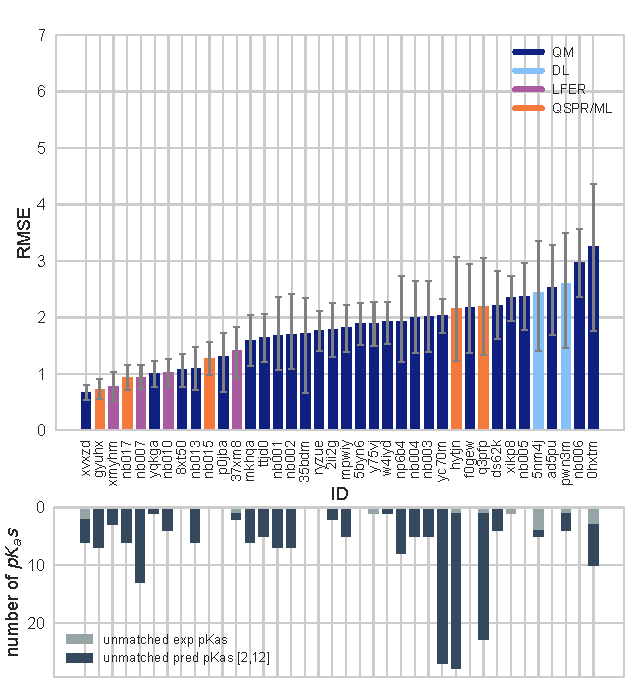
\includegraphics[width=0.5\textwidth]{figures/typeIII-rmse-unmatched-pKa-fig.pdf}}
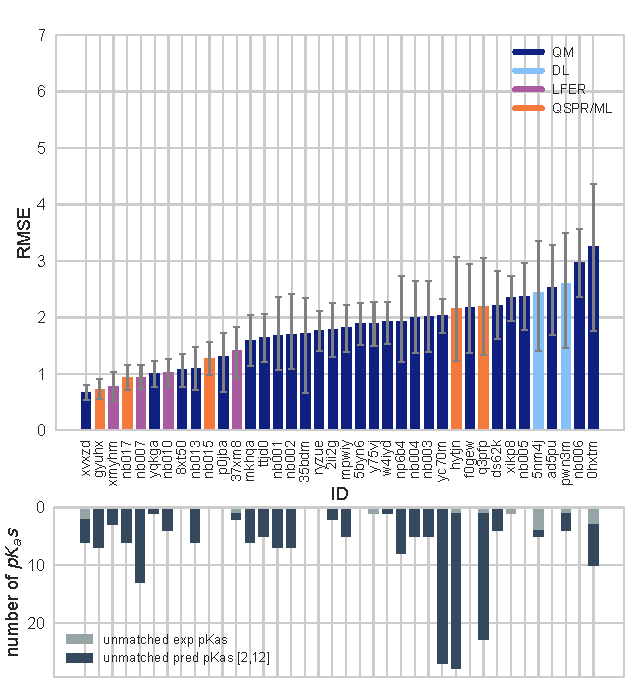
\includegraphics[width=0.5\linewidth]{figures/typeIII-rmse-unmatched-pKa-fig.pdf}
\caption{{\bf RMSE and unmatched \pKa{} counts vs. submission ID plots for macroscopic \pKa{} predictions based on Hungarian matching.} 
Methods are indicated by submission IDs. 
RMSE is shown with error bars denoting 95\% confidence intervals obtained by bootstrapping over challenge molecules. 
Submissions are colored by their method categories. Light blue colored database lookup methods are utilized as the null prediction method.
QM methods category (navy) includes pure QM, QM+LEC, and QM+MM approaches.
Lower bar plots show the number of unmatched experimental \pKa{}~ values (light grey, missing predictions) and the number of unmatched \pKa{} predictions (dark grey, extra predictions) for each method between pH 2 and 12. Submission IDs are summarized in Table~\ref{submission-ID-table}. Submission IDs of the form \textit{nb\#\#\#} refer to non-blinded reference methods computed after the blind challenge submission deadline. All others refer to blind, prospective predictions. 
}
\label{fig:typeIII-rmse-plot}
\end{figure}

The performance of macroscopic \pKa{} predictions was analyzed by comparison to experimental \pKa{} values collected by the spectrophotometric method via numerical matching following the Hungarian method.  
Overall \pKa{} prediction performance was worse than we hoped. 
Fig.~\ref{fig:typeIII-rmse-plot} shows RMSE calculated for each prediction method represented by their submission IDs. 
Other performance statistics are depicted in Fig.~\ref{fig:typeIII-statistics}.
In both figures, method categories are indicated by the color of the error bars. The statistics depicted in these figures can be found in Table~\ref{SI_statistics_table_macro_pKa}.
Prediction error ranged between 0.7 to 3.2 \pKa{} units in terms of RMSE, while an RMSE between 2-3 log units was observed for the majority of methods (20 out of 38 methods). 
Only five methods achieved RMSE less than 1 \pKa{} unit. 
One is QM method with COSMO-RS approach for solvation and linear empirical correction (\textit{xvxzd} (DSD-BLYP-D3(BJ)/def2-TZVPD//PBEh-3c[DCOSMO-RS] + RRHO(GFN-xTB[GBSA]) + Gsolv(COSMO-RS[TZVPD]) and linear fit)), and the remaining four are empirical prediction methods of LFER (\textit{xmyhm} (ACD/pKa Classic), \textit{nb007} (Schr\"{o}dinger/Epik Scan)) and QSPR/ML categories (\textit{gyuhx} (Simulations Plus), \textit{nb017} (MoKa)). 
These five methods with RMSE less than 1 \pKa{} unit are also the methods that have the lowest MAE.
\textit{xmyhm} and \textit{xvxzd} were the only two methods for which the upper 95\% confidence interval of RMSE was lower than 1 \pKa{} unit. 

In terms of correlation statistics, many methods have good performance, although the ranking of methods changes according to R\textsuperscript{2} and Kendall's Tau. 
Therefore, many methods are indistinguishable from one another, considering the uncertainty of the correlation statistics. 
32 out of 38 methods have R\textsuperscript{} and Kendall's Tau higher than 0.7 and 0.6, respectively.
8 methods have R\textsuperscript{2} higher than 0.9 and 6 methods have Kendall's Tau higher than 0.8.
The overlap of these two sets are the following:
\textit{gyuhx} (Simulations Plus), \textit{xvxzd} (DSD-BLYP-D3(BJ)/def2-TZVPD//PBEh-3c[DCOSMO-RS] + RRHO(GFN-xTB[GBSA]) + Gsolv(COSMO-RS[TZVPD]) and linear fit), \textit{xmyhm} (ACD/pKa Classic), \textit{ryzue} (Adiabatic scheme with single point correction: MD/M06-2X//6-311++G(d,p)//M06-2X/6-31+G(d) for bases and SMD/M06-2X//6-311++G(d,p)//M06-2X/6-31G(d) for acids + thermal corrections), and \textit{5byn6} 
(Adiabatic scheme: thermodynamic cycle that uses gas phase optimized structures for gas phase free energy and solution phase geometries for solvent phase free energy. 
SMD/M06-2X/6-31+G(d) for bases and SMD/M06-2X/6-31G(d) for acids + thermal corrections).
It is worth noting that \textit{ryzue} and \textit{5byn6} are QM predictions without any empirical correction. Their high correlation and rank correlation coefficient scores signal that with an empirical correction their accuracy based performance could improve. 
Indeed, the participants have shown that this is the case in their own challenge analysis paper and achieved RMSE of 0.73 \pKa{} units after the challenge~\citep{Zeng:2018:J.Comput.AidedMol.Des.}. 

Null prediction methods based on database lookup (\textit{5nm4j} and \textit{pwn3m}) had similar performance, with an RMSE of roughly 2.5 \pKa{} units, an MAE of 1.5 \pKa{} units, R\textsuperscript{2} of 0.2, and Kendall's Tau of 0.3.
Many methods were observed to have a prediction performance advantage over the null predictions shown in light blue in Fig.~\ref{fig:typeIII-rmse-plot} and Fig.~\ref{fig:typeIII-statistics} considering all the performance metrics as a whole.
In terms of correlation statistics, the null methods are the worst performers, except for \textit{0hxtm}.
From the perspective of accuracy-based statistics (RMSE and MAE), only the top 10 methods were observed to have significantly lower errors than the null methods considering the uncertainty of error metrics expressed as 95\% confidence intervals.

The distribution of macroscopic \pKa{} prediction signed errors observed in each submission was plotted in Fig.~\ref{fig:typeIII-error-distribution}A as ridge plots using the Hungarian matching scheme.
\textit{2ii2g, f0gew, np64b, p0jba}, and \textit{yc70m} tended to overestimate, while  \textit{
5byn6, ryzue}, and \textit{w4iyd} tended to underestimate macroscopic \pKa{} values. 

Four submissions in the QM+LEC category used the COSMO-RS implicit solvation model. 
While three of these achieved the lowest RMSE among QM-based methods (\textit{xvxzd}, \textit{yqkga}, and \textit{8xt50})~\citep{Pracht:2018:J.Comput.AidedMol.Des.}, one of them showed the highest RMSE (\textit{0hxtm} (COSMOtherm\_FINE17)) among all SAMPL6 Challenge macroscopic \pKa{} predictions. 
All four methods used COSMO-RS/FINE17 to compute solvation free energies. 
The major difference between the three low-RMSE methods and \textit{0hxtm} seems to be the protocol for determining relevant conformations for each microstate. 
\textit{xvxzd}, \textit{yqkga}, and \textit{8xt50} used a semi-empirical tight binding (GFN-xTB) method and GBSA continuum solvation model for geometry optimization, followed by high level single-point energy calculations with a solvation free energy correction (COSMO-RS(FINE17/TZVPD)) and rigid rotor harmonic oscillator (RRHO[GFN-xTB(GBSA]) correction. 
\textit{yqkga}, and \textit{8xt50} selected  conformations for each microstate with the Relevant Solution Conformer Sampling and Selection (ReSCoSS) workflow~\citep{Pracht:2018:J.Comput.AidedMol.Des.}. 
The conformations were clustered according to shape, and the lowest energy conformations from each cluster (according to BP86/TZVP/COSMO single point energies in any of the 10 different COSMO-RS solvents) were considered as relevant conformers. 
The \textit{yqkga} method further filtered out conformers that have less than 5\% Boltzmann weights at the DSD-BLYP-D3/def2-TZVPD + RRHO(GFNxTB) + COSMO-RS(fine) level.
The \textit{xvxzd} method used an MF–MD–GC//GFN-xTB workflow and energy thresholds of 6~kcal/mol and 10~kcal/mol, for conformer and microstate selection.
On the other hand, the conformational ensemble captured for each microstate seems to be more limited for the \textit{0hxtm} method, judging by the method description provided in the submission file (this participant did not publish an analysis of the results that they obtained for SAMPL6). 
The \textit{0hxtm} method reported that relevant conformations were computed with the COSMOconf 4.2 workflow which produced multiple relevant conformers for only the neutral states of SM18 and SM22.  
In contrast to \textit{xvxzd}, \textit{yqkga}, and \textit{8xt50}, the \textit{0hxtm} method also did not include a RRHO correction.
Participants who submitted the three low-RMSE methods report that capturing the chemical ensemble for each molecule including conformers and tautomers and high-level QM calculations led to more successful macroscopic \pKa{} prediction results and RRHO correction provided a minor improvement~\citep{Pracht:2018:J.Comput.AidedMol.Des.}. 
Comparing these results to other QM approaches in the SAMPL Challenge also points to the advantage of the COSMO-RS solvation approach compared to other implicit solvent models.

In addition to the statistics related to the \pKa{} value, we also analyzed missing or extra \pKa{} predictions. 
Analysis of the \pKa{} values with accuracy- and correlation-based error metrics was only possible after the matching of predicted macroscopic \pKa{}~ values to experimental \pKa{}~ values through Hungarian matching, although this approach masks \pKa{} prediction issues in the form of extra or missing macroscopic \pKa{} predictions. 
To capture this class of prediction errors, we reported the number of unmatched experimental \pKa{}s (missing \pKa{} predictions) and the number of unmatched predicted \pKa{}s (extra \pKa{} predictions) after Hungarian matching for each method. 
Both missing and extra \pKa{} prediction counts were only considered for the pH range of 2--12, which corresponds to the limits of the experimental assay.
The lower subplot of Fig.~\ref{fig:typeIII-rmse-plot} shows the total count of unmatched experimental or predicted \pKa{}~ values for all the molecules in each prediction set. 
The order of submission IDs in the x-axis follows the RMSD based ranking so that the performance of each method from both \pKa{} value accuracy and the number of \pKa{}s can be viewed together.
The omission or inclusion of extra macroscopic \pKa{} predictions is a critical error because inaccuracy in predicting the correct number of macroscopic transitions shows that methods are failing to predict the correct set of charge states, i.e., failing to predict the correct number of ionization states that can be observed between the specified pH range. 

In the analysis of these challenge results, extra macroscopic \pKa{} predictions were found to be more common than missing \pKa{} predictions. 
In \pKa{} prediction evaluations, the accuracy of predicted ionization states within a pH range is usually neglected. 
When predictions are only evaluated for the accuracy of the \pKa{} value with numerical matching algorithms, a larger number of predicted \pKa{}s lead to greater underestimation of prediction errors. 
Therefore, it is not surprising that methods are biased to predict extra \pKa{} values. 
The SAMPL6 \pKa{} Challenge experimental data consists of 31 macroscopic \pKa{}s in total, measured for 24 molecules (6 molecules in the set have multiple \pKa{}s).
Within the 10 methods with the lowest RMSE, only the \textit{xvxzd} method predicts too few \pKa{} values (2 unmatched out of 31 experimental \pKa{}s). 
All other methods that rank in the top 10 by RMSE have extra predicted \pKa{}s ranging from 1 to 13. 
Two prediction sets without any extra \pKa{} predictions and low RMSE are \textit{8xt50} (ReSCoSS conformations // DSD-BLYP-D3 reranking // COSMOtherm pKa) and \textit{nb015} (ChemAxon/Chemicalize).



\begin{figure}[ht!]
\centering
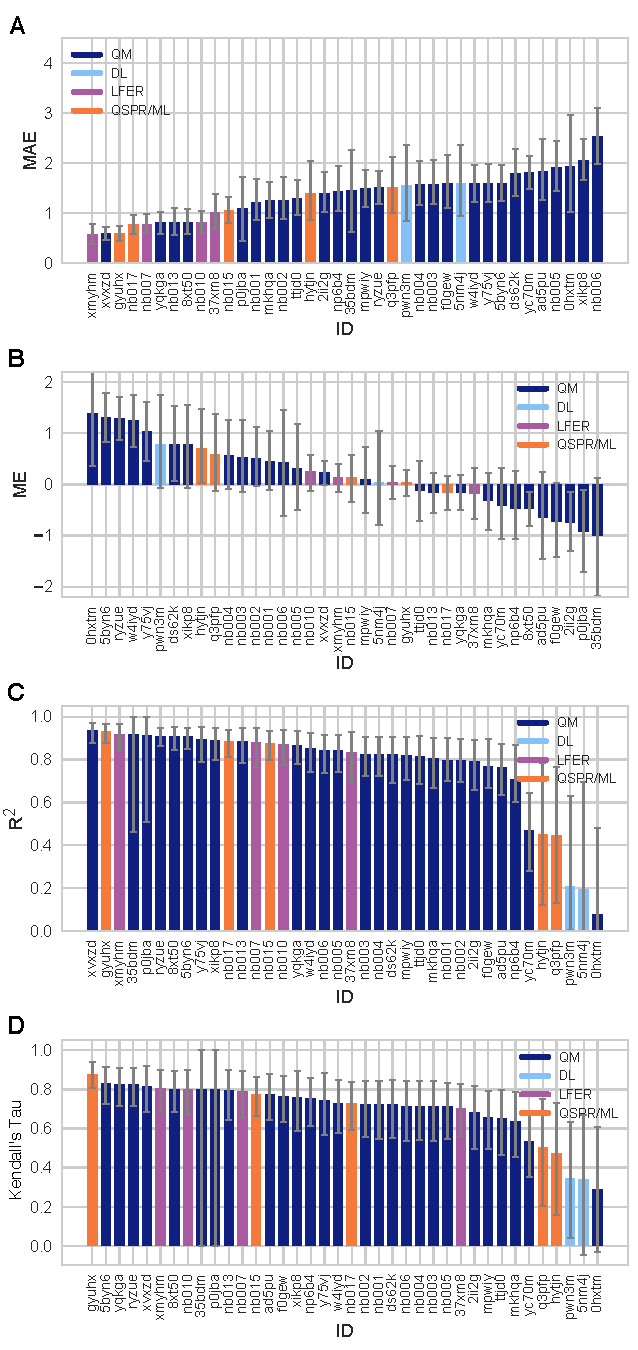
\includegraphics[width=0.5\linewidth]{figures/typeIII_statistics.pdf}
\caption{{\bf Additional performance statistics for macroscopic \pKa{} predictions based on Hungarian matching.} 
Methods are indicated by submission IDs. 
Mean absolute error (MAE), mean error (ME), Pearson’s R\textsuperscript{2}, and Kendall’s Rank Correlation Coefficient Tau ($\tau$) are shown, with error bars denoting 95\% confidence intervals were obtained by bootstrapping over challenge molecules. 
Refer to Table~\ref{submission-ID-table} for the submission IDs and method names. 
Submissions are colored by their method categories. 
Light blue colored database lookup methods are utilized as the null prediction method.
}
\label{fig:typeIII-statistics}
\end{figure}


\subsubsection{Consistently well-performing methods for macroscopic \pKa{} prediction}

Methods ranked differently when ordered by different error metrics, although there were a couple of methods that consistently ranked in the top fraction. 
By using combinatorial criteria that take multiple statistical metrics and unmatched \pKa{} counts into account, we identified a shortlist of consistently well-performing methods for macroscopic \pKa{} predictions, shown in Table~\ref{typeIII-well-performing-methods-table}. 
The criteria for selection were the overall ranking in Top~10 according to RMSE, MAE, R\textsuperscript{2}, and Kendall's Tau and also having a combined unmatched \pKa{} (extra and missing \pKa{}s) count less than 8 (a third of the number of compounds). We ranked methods in ascending order for RMSE and MAE and in descending order for R\textsuperscript{2}, and Kendall's Tau to determine methods. 
Then, we took the intersection set of Top 10 methods according to each statistic to determine the consistently-well performing methods.
This resulted in a list of four methods that are consistently well-performing across all criteria.

Consistently well-performing methods for macroscopic \pKa{} prediction included methods from all categories. 
Two methods in the QM+LEC category were \textit{xvxzd} (DSD-BLYP-D3(BJ)/def2-TZVPD//PBEh-3c[DCOSMO-RS] + RRHO(GFN-xTB[GBSA]) + Gsolv(COSMO-RS[TZVPD]) and linear fit) and \textit(8xt50) (ReSCoSS conformations // DSD-BLYP-D3 reranking // COSMOtherm pKa) and both used COSMO-RS. 
Empirical \pKa{} predictions with top performance were both proprietary software. 
From QSPR and LFER categories, \textit{gyuhx} (Simulations Plus) and \textit{xmymhm} (ACD/pKa Classic) were consistently well-performing methods. 
The Simulation Plus \pKa{} prediction method consisted of 10 artificial neural network ensembles trained on 16,000 compounds for 10 classes of ionizable atoms, with the ionization class of each atom determined using an assigned atom type and local molecular environment~\citep{simulation_plus_D3R_presentation}. 
The ACD/pKa Classic method was trained on 17,000 compounds, uses Hammett-type equations, and captures effects related to tautomeric equilibria, covalent hydration, resonance effects, and  $\alpha, \beta$-unsaturated systems ~\citep{ACD-pKa-classic}.


\begin{table}[h]
\begin{center}
\begin{threeparttable}
\centering\scriptsize
\caption{{\bf Four consistently well-performing prediction methods for macroscopic \pKa{} prediction based on consistent ranking within the Top~10 according to various statistical metrics.} 
Submissions were ranked according to RMSE, MAE, R\textsuperscript{2}, and $\tau$. 
Consistently well-performing methods were selected as the ones that rank in the Top~10 in each of these statistical metrics. 
These methods also have less than 2 unmatched experimental \pKa{}s and less than 7 unmatched predicted \pKa{}s according to Hungarian matching. 
Performance statistics are provided as mean and 95\% confidence intervals.
} 
\label{typeIII-well-performing-methods-table}
\begin{tabular}{@{}llllllll@{}}
\toprule
\textbf{Submission ID} & \textbf{Method Name} & \textbf{RMSE} & \textbf{MAE} & \textbf{R\textsuperscript{2}} & \textbf{\begin{tabular}[c]{@{}l@{}}Kendall's Tau \\ ($\tau$)\end{tabular}} & \textbf{\begin{tabular}[c]{@{}l@{}}Unmatched Exp. \\ \pKa{} Count\end{tabular}} & \textbf{\begin{tabular}[c]{@{}l@{}}Unmatched Pred. \\ \pKa{} Count [2,12]\end{tabular}} \\ \midrule
\rowcolor[HTML]{EFEFEF} 
\textit{xvxzd} & \begin{tabular}[c]{@{}l@{}}Full quantum chemical calculation of \\ free energies and fit to experimental pKa\end{tabular} & 0.68 [0.54, 0.81] & 0.58 [0.45, 0.71] & 0.94 [0.88, 0.97] & 0.82 [0.68, 0.92] & 2 & 4 \\
\textit{gyuhx} & S+pKa & 0.73 [0.55, 0.91] & 0.59 [0.44, 0.74] & 0.93 [0.88, 0.96] & 0.88 [0.8, 0.94] & 0 & 7 \\
\rowcolor[HTML]{EFEFEF} 
\textit{xmyhm} & ACD/pKa Classic & 0.79 [0.52, 1.03] & 0.56 [0.38, 0.77] & 0.92 [0.85, 0.97] & 0.81 [0.68, 0.9] & 0 & 3 \\
\textit{8xt50} & \begin{tabular}[c]{@{}l@{}}ReSCoSS conformations // DSD-BLYP-D3 \\ reranking // COSMOtherm pKa\end{tabular} & 1.07 [0.78, 1.36] & 0.81 [0.58, 1.07] & 0.91 [0.84, 0.95] & 0.80 [0.68, 0.89] & 0 & 0 \\ \bottomrule
\end{tabular}
\end{threeparttable}
\end{center}
\end{table}

Figure~\ref{fig:typeIII_pred_vs_exp_correlation} plots predicted vs.\ experimental macroscopic \pKa{} predictions of four consistently well-performing methods, a representative average method, and the null method(\textit{5nm4j}). 
We selected the method with the highest RMSE below the median of all methods as the representative method with average performance: \textit{2ii2g} (EC-RISM/MP2/cc-pVTZ-P2-q-noThiols-2par).

\begin{figure}[h]
\centering
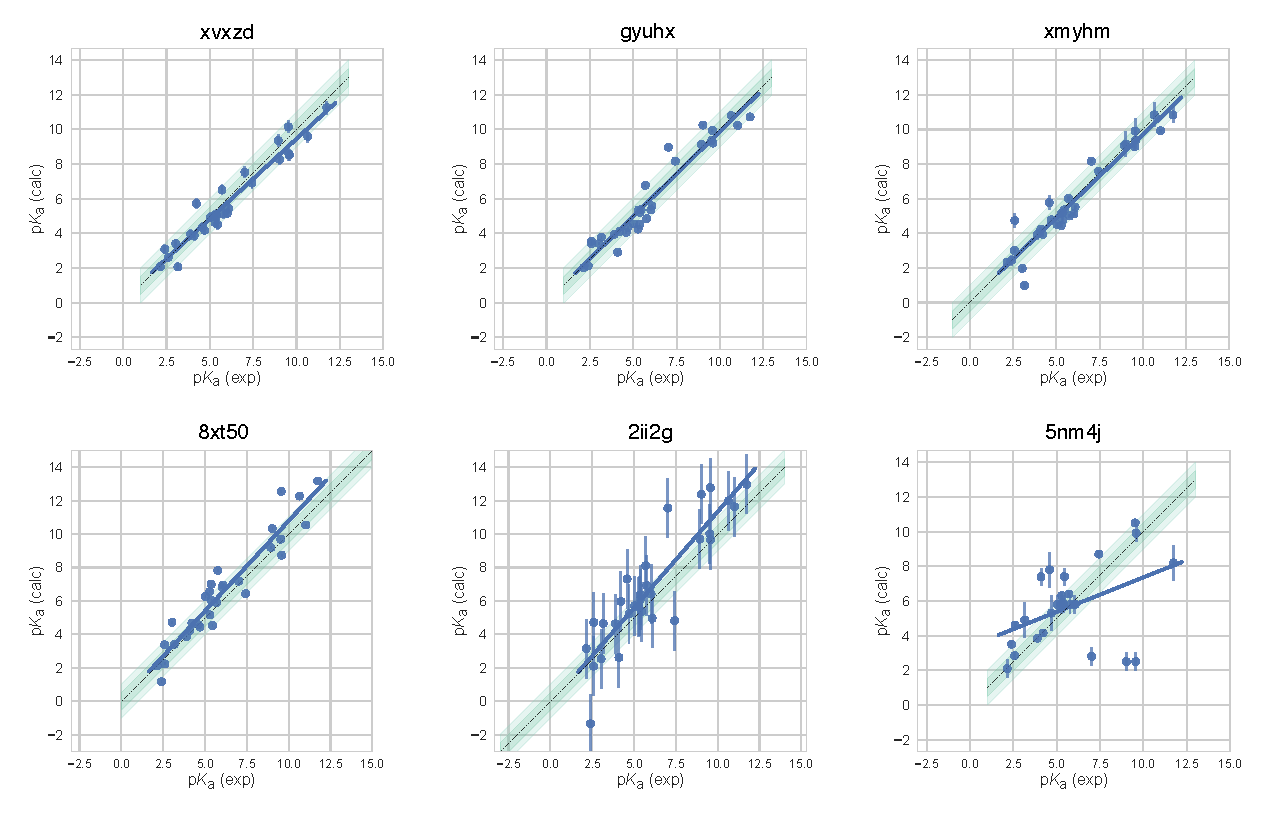
\includegraphics[width=1.0\linewidth]{figures/typeIII-pred-vs-exp-correlation-fig.pdf}
\caption{{\bf Predicted vs.\ experimental macroscopic \pKa{} prediction for four consistently well-performing methods, a representative method with average performance (\textit{2ii2g}), and the null method (\textit{5nm4j})}. 
When submissions were ranked according to RMSE, MAE, R\textsuperscript{2}, and $\tau$, four methods ranked in the Top~10 consistently in each of these metrics.
Dark and light green shaded areas indicate 0.5 and 1.0 units of error. Error bars indicate standard error of the mean of predicted and experimental values. Experimental \pKa{} SEM values are too small to be seen under the data points. EC-RISM/MP2/cc-pVTZ-P2-q-noThiols-2par method (\textit{2ii2g}) was selected as the representative method with average performance because it is the method with the highest RMSE below the median.
}
\label{fig:typeIII_pred_vs_exp_correlation}
\end{figure}



\subsubsection{Which chemical properties are driving macroscopic \pKa{} prediction failures?}

In addition to comparing the performance of methods that participated in the SAMPL6 Challenge, we also wanted to analyze macroscopic \pKa{} predictions from the perspective of challenge molecules and determine whether particular compounds suffer from larger inaccuracy in \pKa{} predictions. 
The goal of this analysis is to provide insight on which molecular properties or moieties might be causing larger \pKa{} prediction errors. 
In Fig.~\ref{fig:molecules_with_MAE_of_all_methods}, 2D depictions of the challenge molecules are presented with MAE calculated for their macroscopic \pKa{} predictions over all methods, based on Hungarian match. 
For multiprotic molecules, the MAE was averaged over all the \pKa{}~ values. 
For the analysis of \pKa{} prediction accuracy observed for each molecule, MAE is a more appropriate statistical value than RMSE for following global trends, as it is less sensitive to outliers than the RMSE.

A comparison of the prediction accuracy of individual molecules is shown in Fig.~\ref{fig:typeIII_molecular_MAE}. 
In Fig.~\ref{fig:typeIII_molecular_MAE}A, the MAE for each molecule is shown considering all blind predictions and reference calculations. 
A cluster of molecules marked orange and red have higher than average MAE. 
Molecules marked red (SM06, SM21, and SM22) are the only compounds in the SAMPL6 dataset with bromo or iodo groups and they suffered a macroscopic \pKa{} prediction error in the range of 1.7--2.0 \pKa{} units in terms of MAE.
Molecules marked orange (SM03, SM10, SM18, SM19, and SM20) have sulfur-containing heterocycles, and all these molecules except SM18 have MAE larger than 1.6 \pKa{} units.
Despite containing a thiazole group, SM18 has a low prediction MAE.
SM18 is the only compound with three experimental \pKa{}~ values, and we suspect the presence of multiple experimental \pKa{}~ values could have a masking effect on the errors captured by the MAE when the Hungarian matching scheme is used due to more potential pairing choices that may artificially lower the error.

We separately analyzed the MAE of each molecule for empirical (LFER and QSPR/ML) and QM-based physical methods (QM, QM+LEC, and QM+MM) to gain additional insight into prediction errors. 
Fig.~\ref{fig:typeIII_molecular_MAE}B shows that the difficulty of predicting \pKa{}~ values of the same subset of molecules was a trend conserved in the performance of physical methods.
For QM-based methods, sulfur-containing heterocycles, amides proximal to aromatic heterocycles, and compounds with iodo and bromo substitutions have lower \pKa{} prediction accuracy.

The SAMPL6 \pKa{} set consists of only 24 small molecules and lacks multiple examples of many moieties, limiting our ability to determine with statistical significance which chemical substructures cause greater errors in \pKa{} predictions. 
Still, the trends observed in this challenge point to molecules with iodo-, bromo-, and sulfur-containing heterocycles as having systematically larger prediction errors in macroscopic \pKa{} value. 
We hope that reporting this observation will lead to the improvement of methods for similar compounds with such moieties. 





\begin{figure}
\centering
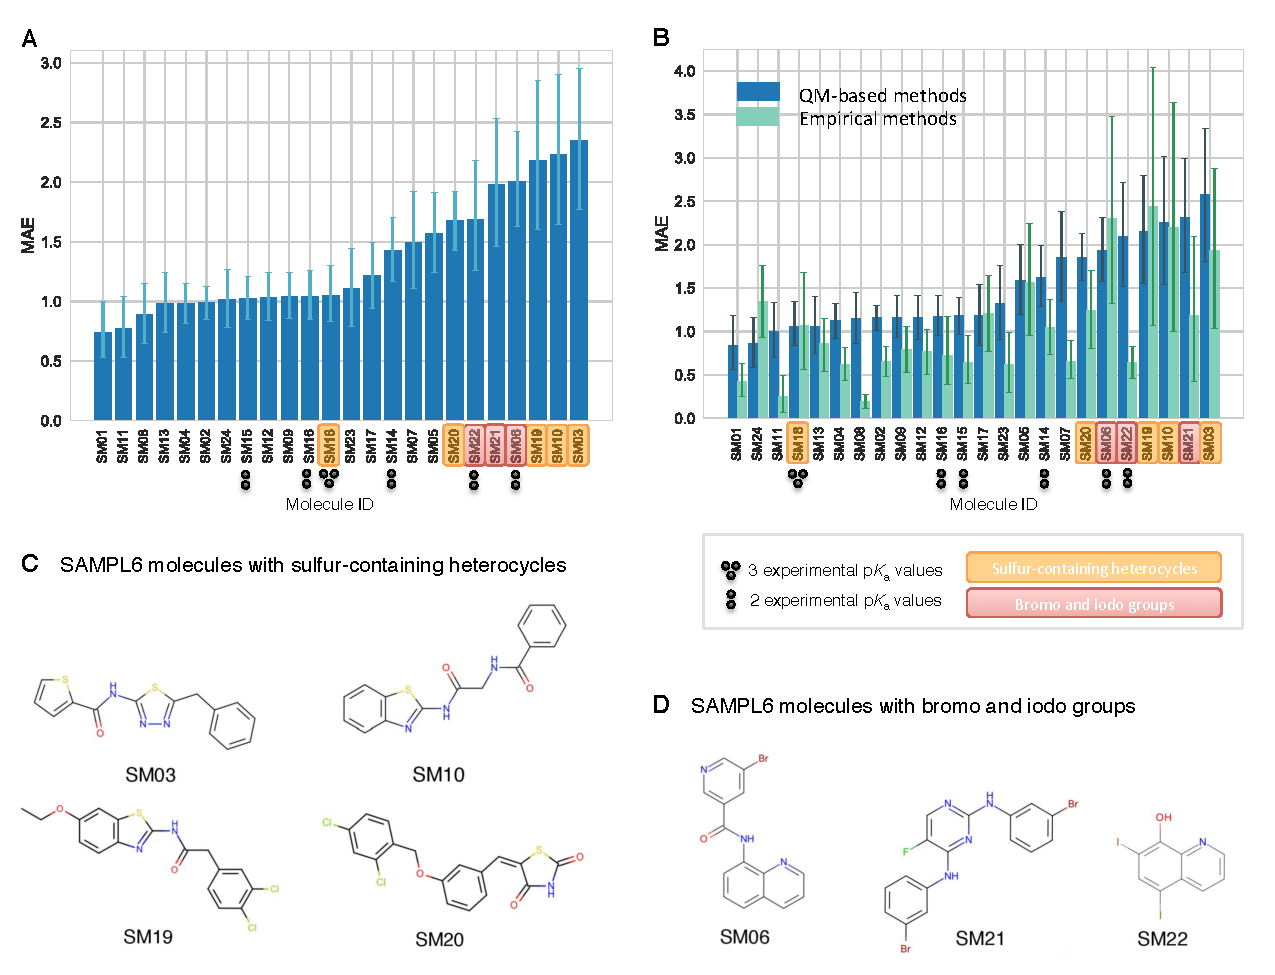
\includegraphics[width=1.0\linewidth]{figures/typeIII_molecular_MAE_fig.pdf}
\caption{{\bf Average prediction accuracy calculated over all prediction methods was poorer for molecules with sulfur-containing heterocycles, bromo, and iodo groups.}
{\bf(A)} MAE calculated for each molecule as an average of all methods. 
{\bf(B)} MAE of each molecule broken out by method category. QM-based methods (blue) include QM predictions with or without linear empirical correction. 
Empirical methods (green) include QSAR, ML, DL, and LFER approaches. 
{\bf(C)} Depiction of SAMPL6 molecules with sulfur-containing heterocycles. 
{\bf(D)} Depiction of SAMPL6 molecules with iodo and bromo groups.
}
\label{fig:typeIII_molecular_MAE}
\end{figure}


\begin{figure}
\centering
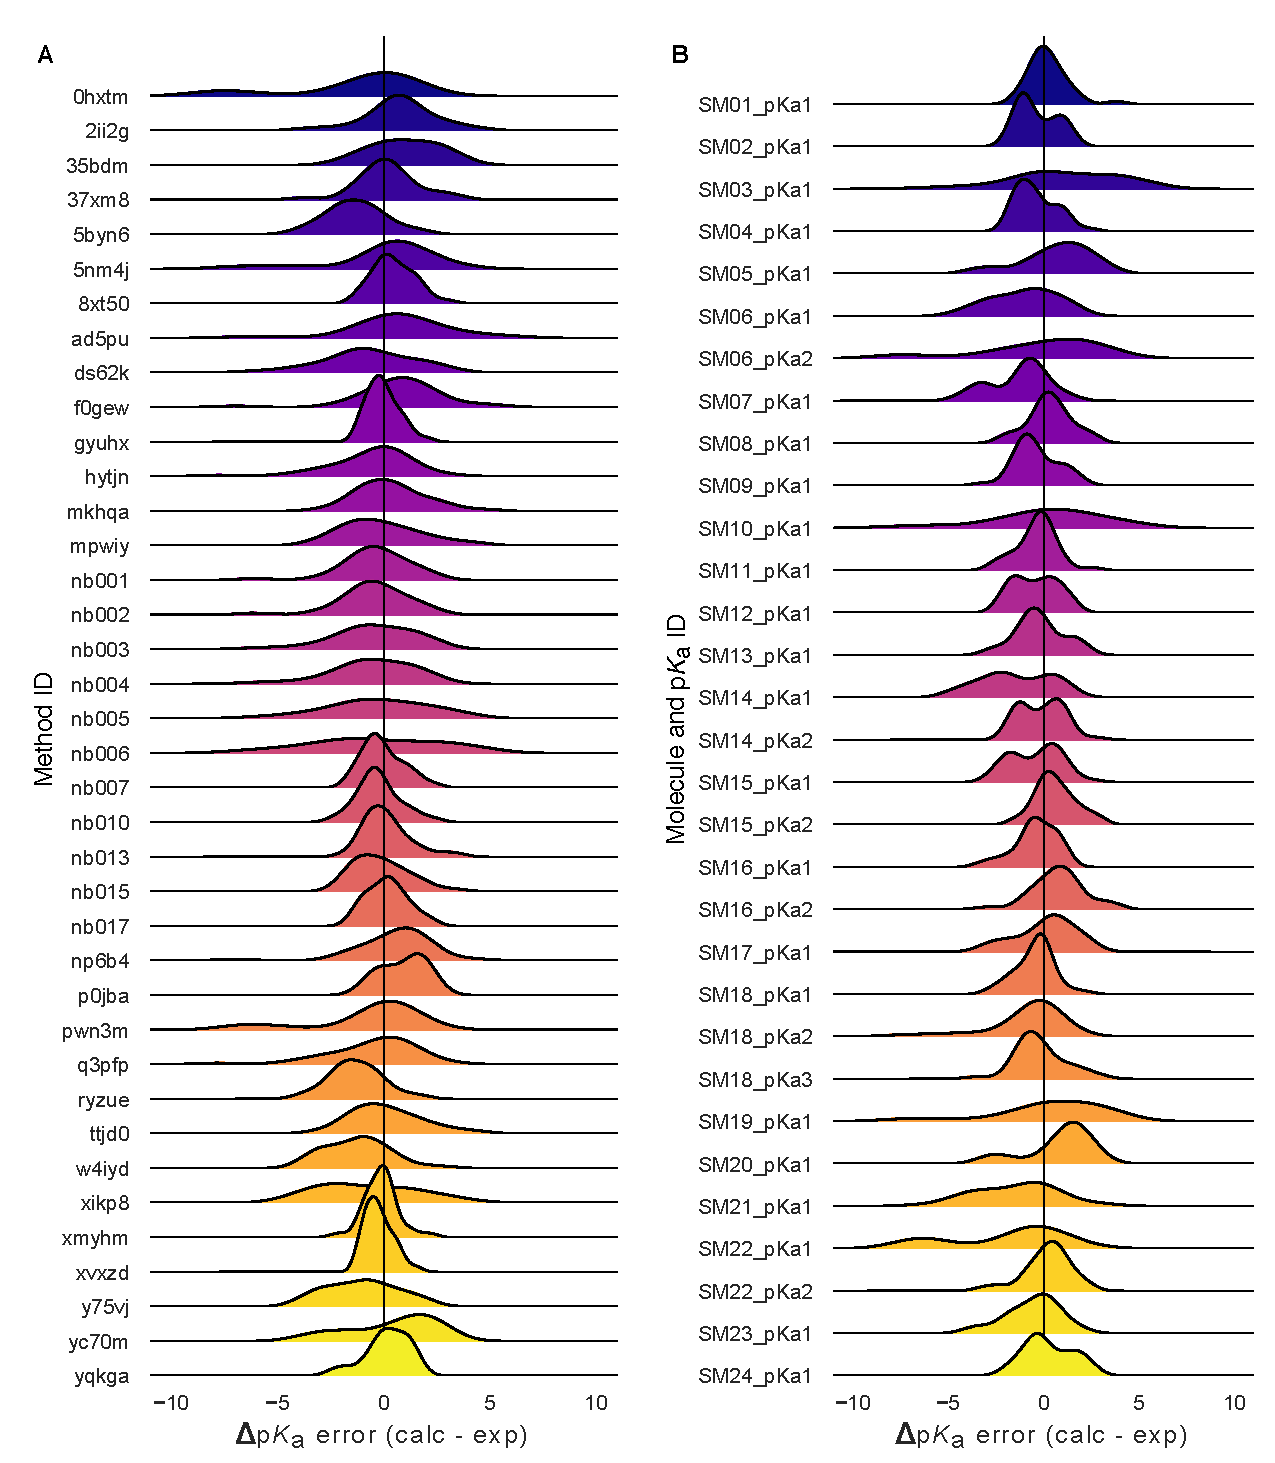
\includegraphics[width=0.8\linewidth]{figures/typeIII-error-distribution.pdf}
\caption{{\bf Macroscopic \pKa{} prediction error distribution plots show how prediction accuracy varies across methods and individual molecules.}
{\bf(A)} \pKa{} prediction error distribution for each submission for all molecules according to Hungarian matching. 
{\bf(B)} Error distribution for each SAMPL6 molecule for all prediction methods according to Hungarian matching. For multiprotic molecules, \pKa{} ID numbers (pKa1, pKa2, and pKa3) were assigned in the direction of increasing experimental \pKa{} value. 
}
\label{fig:typeIII-error-distribution}
\end{figure}

We have also looked for correlation with molecular descriptors for finding other potential explanations as to why macroscopic \pKa{} prediction errors were larger for certain molecules. 
While testing the correlation between errors and many molecular descriptors, it is important to account for the possibility of spurious correlations. 
We haven't observed any statistically significant correlation between numerical \pKa{} predictions and the descriptors we have tested. 
First, having more experimental \pKa{}~ values (Fig.~\ref{fig:typeIII_molecular_MAE}A) did not seem to be associated with poorer \pKa{} prediction performance. 
Still, we need to keep in mind that multiprotic compounds were sparsely represented in the SAMPL6 set (5 molecules with 2 macroscopic \pKa{}~ values and one with 3 macroscopic \pKa{}).
Second, we checked the following other descriptors: presence of an amide group, molecular weight, heavy atom count, rotatable bond count, heteroatom count, heteroatom-to-carbon ratio, ring system count, maximum ring size, and the number of microstates (as enumerated for the challenge). 
Correlation plots and R\textsuperscript{2} values can be seen in Fig.~\ref{fig:molecular_properties_vs_MAE_correlation}. 

We had suspected that \pKa{} prediction methods may perform better for moderate values (4--10) than extreme values as molecules with extreme \pKa{}~ values are less likely to change ionization states close to physiological pH. 
To test this we look at the distribution of absolute errors calculated for all molecules and challenge predictions binned by experimental \pKa{} value 2 \pKa{} unit increments. 
As can be seen in Fig.~\ref{fig:macroscopic-pKa-error-vs-pKa-value}B, the value of true macroscopic \pKa{}~ values was not a factor affecting the prediction error seen in SAMPL6 Challenge.

Fig.~\ref{fig:typeIII-error-distribution}B is helpful to answer the question "Are there molecules with consistently overestimated or underestimated \pKa{}~ values?". 
This ridge plots show the error distribution of each experimental \pKa{}. 
SM02\_pKa1, SM04\_pKa1, SM14\_pKa1, and SM21\_pKa1 were underestimated, predicting lower protein affinity by more than 1 \pKa{} unit by majority of the prediction methods. 
SM03\_pKa1, SM06\_pKa2, SM19\_pKa1, and SM20\_pKa1 were overestimated by the majority of the prediction methods by more than 1 \pKa{} unit.
SM03\_pKa1, SM06\_pKa2, SM10\_pKa1, SM19\_pKa1, and SM22\_pKa1 have the highest spread of errors and were less accurately predicted overall. 



%%%
\subsection{Analysis of microscopic \pKa{} predictions using microstates determined by NMR for 8 molecules}

The most common approach for analyzing microscopic \pKa{} prediction accuracy has been to compare it to experimental macroscopic \pKa{} data, assuming experimental \pKa{}~ values describe titrations of distinguishable sites and, therefore, correspond to microscopic \pKa{}s. 
But this typical approach fails to evaluate methods at the microscopic level.

Analysis of microscopic \pKa{} predictions for the SAMPL6 Challenge was not straightforward due to the lack of experimental data with microscopic resolution of the titratable sites and their associated microscopic \pKa{}s. 
For 24 molecules, macroscopic \pKa{}~ values were determined with the spectrophotometric method. 
For 18 molecules, a single macroscopic titration was observed, and for 6 molecules multiple experimental \pKa{}~ values were observed and characterized. 
For 18 molecules with a single experimental \pKa{}, it is probable that the molecules are monoprotic and, therefore, macroscopic \pKa{} value is equal to the microscopic \pKa{}.
There is, however, no direct experimental evidence supporting this hypothesis aside from the support from computational predictions, such as the predictions by ACD/pKa Classic. 
There is always the possibility that the macroscopic \pKa{} observed is the result of two different titrations overlapping closely with respect to pH if any charge state has more than one tautomer. 
We did not want to bias the blind challenge analysis with any prediction method. 
Therefore, we believe analyzing the microscopic \pKa{} predictions via Hungarian matching to experimental values with the assumption that the 18 molecules have a single titratable site is not the best approach. 
Instead, an analysis at the level of macroscopic \pKa{}~ values is much more appropriate when a numerical matching scheme is the only option to evaluate predictions using macroscopic experimental data.

For a subset of eight molecules, dominant microstates were inferred from NMR experiments. 
Six of these molecules were monoprotic and two were multiprotic.
This dataset was extremely useful for guiding the assignment between experimental and predicted \pKa{} values based on microstates. 
In this section, we present the performance evaluations of microscopic \pKa{} predictions for only the 8 compounds with experimentally-determined dominant microstates.

\begin{figure}
\centering
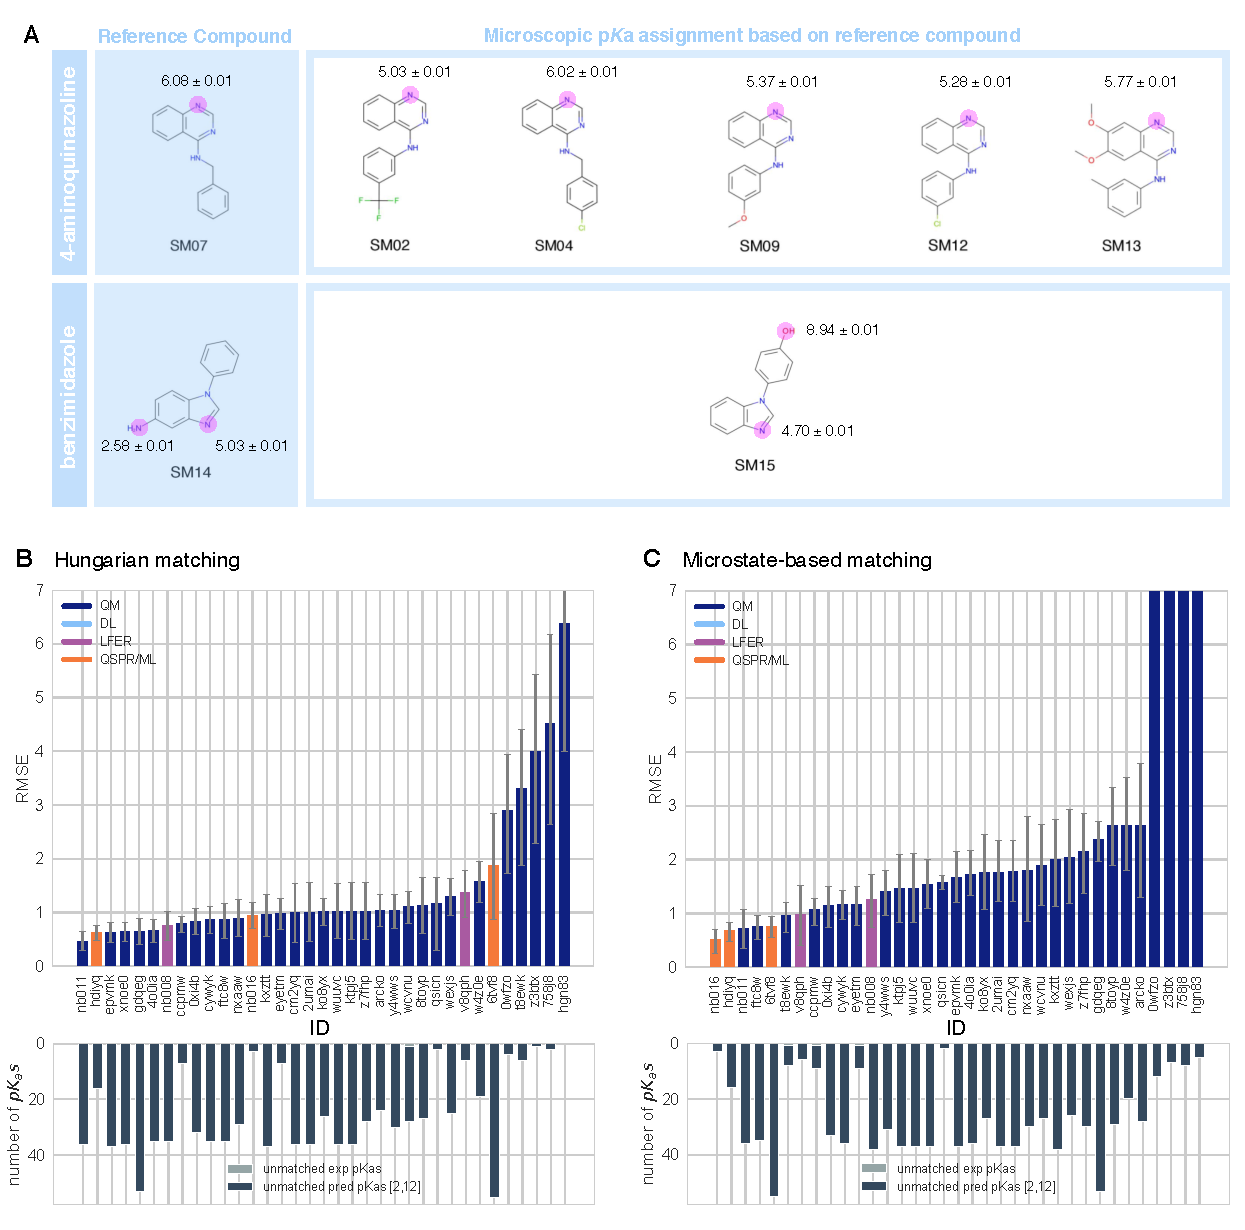
\includegraphics[width=1.0\linewidth]{figures/typeI_8_mol_matching_comparison.pdf}
\caption{{\bf NMR determination of dominant microstates allowed in-depth evaluation of microscopic \pKa{} predictions for 8 compounds.} 
{\bf A} Dominant microstate sequence of two compounds (SM07 and SM14) were determined by NMR~\cite{Isik:2018:J.Comput.AidedMol.Des.}. 
Based on these reference compounds, the dominant microstates of 6 related compounds were inferred and experimental \pKa{} values were assigned to titratable groups with the assumption that only the dominant microstates have significant contributions to the experimentally observed \pKa{}.
{\bf B} RMSE vs.\ submission ID and unmatched \pKa{} vs.\ submission ID plots for the evaluation of microscopic \pKa{} predictions of 8 molecules by Hungarian matching to experimental macroscopic \pKa{}~ values. 
{\bf C} RMSE vs.\ submission ID and unmatched \pKa{} vs.\ submission ID plots showing the evaluation of microscopic \pKa{} predictions of 8 molecules by microstate-based matching between predicted microscopic \pKa{}s and experimental macroscopic \pKa{} values. Submissions \textit{0wfzo, z3btx, 758j8}, and \textit{hgn83} have RMSE values bigger than 10 \pKa{} units which are beyond the y-axis limits of subplot {\bf C} and {\bf B}.
RMSE is shown with error bars denoting 95\% confidence intervals obtained by bootstrapping over the challenge molecules. 
Lower bar plots show the number of unmatched experimental \pKa{}s (light grey, missing predictions) and the number of unmatched \pKa{} predictions (dark grey, extra predictions) for each method between pH 2 and 12. 
Submission IDs are summarized in Table~\ref{submission-ID-table}.
}
\label{fig:typeI-matching-algorithm-comparison}
\end{figure}


\subsubsection{Microstate-based matching revealed errors masked by \pKa{} value-based matching between experimental and predicted \pKa{}s}

Comparing microscopic \pKa{} predictions directly to macroscopic experimental \pKa{} values with numerical matching can lead to underestimation of errors. 
To demonstrate how numerical matching often masks \pKa{} prediction errors, we compared the performance analysis done by Hungarian matching to that from microstate-based matching for 8 molecules presented in Fig.~\ref{fig:typeI-matching-algorithm-comparison}A. 
RMSE calculated for microscopic \pKa{} predictions matched to experimental values via Hungarian matching is shown in Fig.~\ref{fig:typeI-matching-algorithm-comparison}B, while Fig.~\ref{fig:typeI-matching-algorithm-comparison}C shows RMSE calculated via microstate-based matching. 
The Hungarian matching incorrectly leads to significantly (and artificially) lower RMSE compared to microstate-based matching. 
The reason is that the Hungarian matching assigns experimental \pKa{} values to predicted \pKa{} values only based on the closeness of the numerical values, without consideration of the relative population of microstates and microstate identities. 
Because of this, a microscopic \pKa{} value that describes a transition between very low population microstates (high energy tautomers) can be assigned to the experimental \pKa{} if it has the closest \pKa{} value. 
This is not helpful because, in reality, the microscopic \pKa{}~ values that influence the observable macroscopic \pKa{} the most are the ones with higher microstate populations (transitions between low energy tautomers).

The number of unmatched predicted microscopic \pKa{s} is shown in the lower bar plots of Fig.~\ref{fig:typeI-matching-algorithm-comparison}B and C, to emphasize the large number of microscopic \pKa{} predictions submitted by many methods. 
In the case of microscopic \pKa{}, the number of unmatched predictions does not indicate an error in the form of an extra predicted \pKa{}, because the spectrophotometric experiments do not capture all microscopic \pKa{}s theoretically possible (transitions between all pairs of microstates that differ by one proton). 
\pKa{}s of transitions to and from very high energy tautomers are very hard to measure by experimental methods, including the most sensitive methods like NMR. 
Prediction of extra microscopic \pKa{}~ values can cause underestimation of prediction errors when numerical matching algorithms such as Hungarian matching are used. 
We also checked how often Hungarian matching led to the correct matches between predicted and experimental \pKa{} in terms of the microstate pairs, i.e., how often the microstate pair of the Hungarian match recapitulates the dominant microstate pair of the experiment. 
The overall accuracy of microstate pair matching was found to be low for the SAMPL6 Challenge submission. 
Fig.~\ref{fig:microstate-pairs-with-Hungarian-match-vs-experiments} shows that for most methods the predicted microstate pair selected by the Hungarian match did not correspond to the experimentally-determined microstate pair.
This means lower RMSE (better accuracy) performance statistics obtained from Hungarian matching are artificially low. 
This problem could be avoided by matching experimental and predicted values on the basis of microstate IDs, if experimental microscopic assignments are available.  

Unfortunately, we were only able to perform this more reliable microstate-based analysis for a subset of compounds.
The conclusions in this section reflect only eight compounds with limited structural diversity: 
Six molecules with 4-aminoquinazoline and two with benzimidazole scaffolds, with a total of 10 \pKa{} values. 
The sequences of dominant microstates for SM07 and SM14 were determined by NMR experiments directly~\citep{Isik:2018:J.Comput.AidedMol.Des.}, while dominant microstates of their derivatives were inferred by taking them as a reference (Fig.~\ref{fig:typeI-matching-algorithm-comparison}). 
Although we believe that microstate-based evaluation is more informative, the lack of a large experimental dataset limits the conclusions to a very narrow chemical diversity. 
Still, microstate-based matching revealed errors masked by \pKa{} value-based matching between experimental and predicted \pKa{}s.


\subsubsection{Accuracy of \pKa{} predictions evaluated by microstate-based matching}

\begin{figure}
\centering
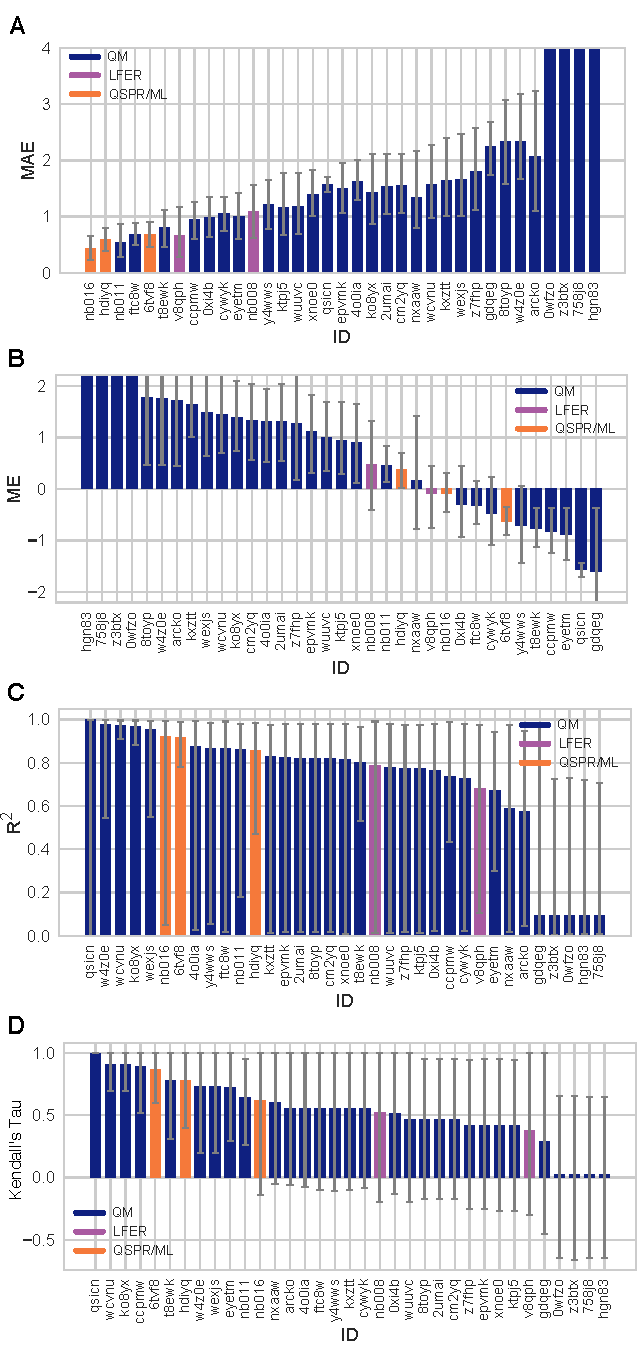
\includegraphics[width=0.5\linewidth]{figures/typeI_statistics.pdf}
\caption{{\bf Additional performance statistics for microscopic \pKa{} predictions for 8 molecules with experimentally determined dominant microstates.} 
Microstate-based matching was performed between experimental \pKa{} values and predicted microscopic \pKa{}~ values. 
Mean absolute error (MAE), mean error (ME), Pearson’s R\textsuperscript{2}, and Kendall’s Rank Correlation Coefficient Tau ($\tau$) are shown, with error bars denoting 95\% confidence intervals obtained by bootstrapping over challenge molecules. 
Methods are indicated by their submission IDs. 
Submissions are colored by their method categories. 
Refer to Table~\ref{submission-ID-table} for submission IDs and method names. Submissions \textit{0wfzo, z3btx, 758j8}, and \textit{hgn83} have MAE and ME values bigger than 10 \pKa{} units which are beyond the y-axis limits of subplots {\bf A} and {\bf B}. 
A large number and wide variety of methods have statistically indistinguishable performance based on correlation statistics ({\bf C} and {\bf D}), in part because of the relatively small dynamic range and small size of the set of 8 molecules.
}
\label{fig:typeI-statistics}
\end{figure}

Both accuracy- and correlation-based statistics were calculated for the predicted microscopic \pKa{} values after microstate-based matching. 
RMSE, MAE, ME, R\textsuperscript{2}, and Kendall's Tau results of each method are shown in Fig.~\ref{fig:typeI-matching-algorithm-comparison}C and Fig.~\ref{fig:typeI-statistics}. 
A table of the calculated statistics can be found in Table~\ref{SI-statistics-table-micro-pKa-8mol-microstate}. 
Due to the small number of data points in this set, correlation-based statistics have large uncertainties and thus have less utility for distinguishing better-performing methods. 
Therefore, we focused more on accuracy-based metrics for the analysis of microscopic \pKa{}s than correlation-based metrics. 
In terms of accuracy of predicted microscopic \pKa{} values, all three QSPR/ML based methods (\textit{nb016} (MoKa), \textit{hdiyq} (Simulations Plus), \textit{6tvf8} (OE Gaussian Process)), three QM-based methods (\textit{nb011} (Jaguar), \textit{ftc8w} (EC-RISM/MP2/cc-pVTZ-P2-q-noThiols-2par), \textit{t8ewk} (COSMOlogic\_FINE17)), and one LFER method (\textit{v8qph} (ACD/pKa GALAS)) achieved RMSE lower than 1 \pKa{} unit. 
The same six methods also have the lowest MAE.


\subsubsection{Evaluation of dominant microstate prediction accuracy}

For many computational chemistry approaches, including structure-based modeling of protein-ligand interactions, predicting the ionization state and the exact position of protons is necessary to establish what to include in the modeled system.  
In addition to being able to predict \pKa{} values accurately, we require \pKa{} prediction methods to be able to capture microscopic protonation states accurately. 
Even when the predicted \pKa{} value is accurate, the predicted protonation sites can be incorrect, leading to potentially large modeling errors in quantities such as the computed free energy of binding. 
Therefore, we assessed whether methods participating in the SAMPL6 \pKa{} Challenge were correctly predicting the sequence of dominant microstates, i.e., dominant tautomers of each charge state observed between pH 2 and 12.

Fig.~\ref{fig:typeI_dominant_microstate_accuracy} shows how well methods perform for predicting the dominant microstate, as analyzed for eight compounds with available experimental microstate assignments.
The dominant microstate sequence is essentially the sequence of states that are most visible experimentally due to their higher fractional population and relative free energy within the tautomers at each charge.
To extract the dominant tautomers predicted for the sequence of ionization states of each method, the relative free energy of microstates were first calculated at reference pH 0~\citep{Gunner:2020:J.Comput.AidedMol.Des.}. 
To subsequently determine the dominant microstate at each formal charge, we selected the lowest energy tautomer for each ionization state based on the relative microstate free energies calculated at pH 0. 
The choice of reference pH is arbitrary, as relative free energy difference between tautomers of the same charge is always constant with respect to pH. 
This analysis was performed only for the charges -1, 0, 1, and 2---the charge range captured by NMR experiments.
Predicted and experimental dominant microstates were then compared for each charge state to calculate the fraction of correctly predicted dominant tautomers. 
This value is reported as the \emph{dominant microstate accuracy} for all charge states (Fig.~\ref{fig:typeI_dominant_microstate_accuracy}A). 

Many of the methods which participated in the challenge made errors in predicting the dominant microstate. 
10 QM and 3 QSPR/ML methods did not make any mistakes in dominant microstate predictions, although, they are expected to make mistakes in the relative population of tautomers (free energy difference between microstates) as reflected by the \pKa{} value errors. 
While all participating QSPR/ML methods showed good performance in dominant microstate prediction, LFER and some QM methods made mistakes. 
The accuracy of the predicted dominant neutral tautomers was perfect for all methods, except \textit{qsicn} (Fig.~\ref{fig:typeI_dominant_microstate_accuracy}B), but errors in predicting the major tautomer of charge +1 were much more frequent. 
22 out of 35 prediction sets made at least one error in predicting the lowest energy tautomer with +1 charge. 
We didn't include ionization states with charges -1 and +2 in this assessment because we had only one compound with these charges in the dataset. 
Nevertheless, errors in predicting the dominant tautomers seem to be a bigger problem for charged tautomers than the neutral tautomer.    

Only eight compounds had data on the sequence of dominant microstates. 
Therefore conclusions on the performance of methods in terms of dominant tautomer prediction are limited to this limited chemical diversity (benzimidazole and 4-aminoquinazoline derivatives). 
We present this analysis as a prototype of how microscopic \pKa{} predictions should be evaluated.
Hopefully, future evaluations can be performed with larger experimental datasets following the strategy we demonstrated here in order to reach broad conclusions about which methods are better for capturing dominant microstates and ratios of tautomers. 
Even if experimental microscopic \pKa{} measurement data is not available, experimental dominant tautomer determinations are still informative for assessing computational predictions.  
  

\begin{figure}[h!]
\centering
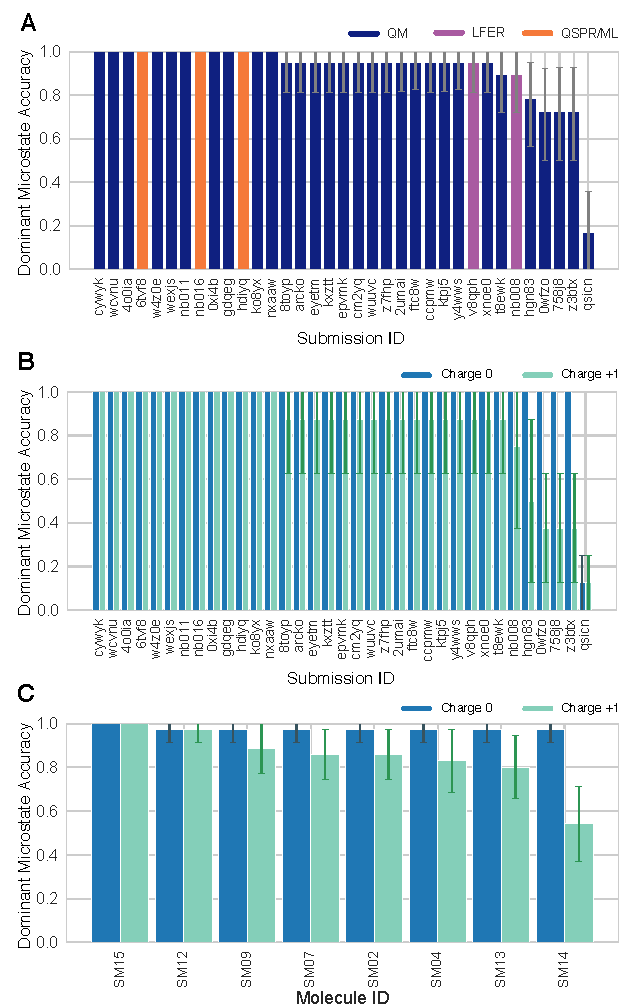
\includegraphics[width=1.0\linewidth]{figures/typeI_dominant_microstate_accuracy.pdf}
\caption{{\bf Some methods predicted the sequence of dominant tautomers inaccurately.} 
Prediction accuracy of the dominant microstate of each charged state was calculated using the dominant microstate sequence determined by NMR for 8 molecules as reference. 
{\bf(A)} Dominant microstate accuracy vs.\ submission ID plot was calculated considering all the dominant microstates seen in the experimental microstate dataset of 8 molecules. {\bf(B)} Dominant microstate accuracy vs. submission ID plot was generating considering only the dominant microstates of charge 0 and +1 seen in the 8 molecule dataset. 
The accuracy of each molecule is broken out by the total charge of the microstate. 
{\bf(C)} Dominant microstate prediction accuracy calculated for each molecule averaged over all methods. 
In {\bf(B)} and {\bf(C)}, the accuracy of predicting the dominant neutral tautomer is shown in blue and the accuracy of predicting the dominant +1 charged tautomer is shown in green. Error bars denoting 95\% confidence intervals obtained by bootstrapping.
{\bf(D)} Depiction of SM14 microstates for protonation states with +2, +1, and 0 charges. The dominant tautomer of each macroscopic protonation state is highlighted with a rectangle. Dominant microstates of each charge were determined based on NMR experiments~\citep{Isik:2018:J.Comput.AidedMol.Des.}.
}
\label{fig:typeI_dominant_microstate_accuracy}
\end{figure}

The most frequent misprediction was the major tautomer of the SM14 cationic form, as shown in Fig.~\ref{fig:typeI_dominant_microstate_accuracy}. 
This figure shows the accuracy of the predicted dominant microstate calculated for individual molecules and for charge states 0 and +1, averaged over all prediction methods. 
SM14, the molecule that exhibits the most frequent error in the predicted dominant microstate, has two experimental \pKa{} values that were 2.4 \pKa{} units apart, and we suspect that could be a contributor to the difficulty of predicting microstates accurately. 
Other molecules are monoprotic (4-aminoquinazolines) or their experimental \pKa{} values are very well separated (SM14, 4.2 \pKa{} units). 
It would be very interesting to expand this assessment to a larger variety of drug-like molecules to discover for which structures tautomer predictions are more accurate and for which structures computational predictions are not as reliable.


\subsubsection{Consistently well-performing methods for microscopic \pKa{} predictions}

We have identified different criteria for determining consistently top-performing predictions of microscopic \pKa{} than macroscopic \pKa{}: having perfect dominant microstate prediction accuracy, unmatched \pKa{} count of 0, and ranking in the top 10 according to RMSE and MAE. 
Correlation statistics were not found to have utility for discriminating performance due to large uncertainties in these statistics for a small dataset of 10 \pKa{} values. 
Unmatched predicted \pKa{} count was also not considered since experimental data was only informative for the \pKa{} between dominant microstates and did not capture all the possible theoretical transitions between microstate pairs. 
Table~\ref{typeI-well-performing-methods-table} reports six methods that have consistent good performance according to many metrics, although evaluated only for the 8 molecule set due to limitations of the experimental dataset. 
Six methods were divided evenly between methods of QSPR/ML category and QM category. 
\textit{nb016} (MoKa), \textit{hdiyq} (Simulations Plus), and \textit{6tvf8} (OE Gaussian Process) were QSPR and ML methods that performed well. 
\textit{nb011} (Jaguar), \textit{0xi4b}(EC-RISM/B3LYP/6-311+G(d,p)-P2-phi-noThiols-2par), and \textit{cywyk} (EC-RISM/B3LYP/6-311+G(d,p)-P2-phi-noThiols-2par) were QM predictions with linear empirical corrections with good performance with microscopic \pKa{} predictions. 

The Simulations Plus \pKa{} prediction method is the only method that appeared to be consistently well-performing in both the assessment for macroscopic and microscopic \pKa{} prediction (\textit{gyuhx} and \textit{hdiyq}). 
However, it is worth noting that two methods that were in the list of consistently top-performing methods for macroscopic \pKa{} predictions lacked equivalent submissions of their underlying microscopic \pKa{} predictions, and therefore could not be evaluated at the microstate level. 
These methods were \textit{xmyhm} (ACD/pKa Classic) and \textit{xvxzd}(DSD-BLYP-D3(BJ)/def2-TZVPD//PBEh-3c[DCOSMO-RS] + RRHO(GFN-xTB[GBSA]) + Gsolv(COSMO-RS[TZVPD]) and linear fit). 


\begin{table}[h]
\begin{center}
\begin{threeparttable}
\centering\scriptsize
\caption{{\bf Top-performing methods for microscopic \pKa{} predictions based on consistent ranking within the Top~10 according to various statistical metrics calculated for 8 molecule dataset.} 
Performance statistics are provided as mean and 95\% confidence intervals. 
Submissions that rank in the Top~10 according to RMSE and MAE and have perfect dominant microstate prediction accuracy were selected as consistently well-performing methods. 
Correlation-based statistics (R\textsuperscript{2}, and Kendall's Tau), although reported in the table, were excluded from the statistics used for determining top-performing methods. 
This was because correlation-based statistics were not very discriminating due to the narrow dynamic range and the small number of data points in the 8 molecule dataset with NMR-determined dominant microstates. 
} 
\label{typeI-well-performing-methods-table}
\begin{tabular}{@{}lllllllll@{}}
\toprule
\textbf{\begin{tabular}[c]{@{}l@{}}Submission\\ ID\end{tabular}} & \textbf{Method Name} & \textbf{\begin{tabular}[c]{@{}l@{}}Dominant \\ Microstate \\ Accuracy\end{tabular}} & \textbf{RMSE} & \textbf{MAE} & \textbf{R\textsuperscript{2}} & \textbf{Kendall's Tau} & \textbf{\begin{tabular}[c]{@{}l@{}}Unmatched \\ Exp. \pKa{} \\ Count\end{tabular}} & \textbf{\begin{tabular}[c]{@{}l@{}}Unmatched \\ Pred. \pKa{} \\ Count [2,12]\end{tabular}} \\ \midrule
\rowcolor[HTML]{EFEFEF} 
{\color[HTML]{000000} \textit{nb016}} & {\color[HTML]{000000} MoKa} & {\color[HTML]{000000} 1.0 [1.0, 1.0]} & {\color[HTML]{000000} 0.52 [0.25, 0.71]} & {\color[HTML]{000000} 0.43 [0.23, 0.65]} & {\color[HTML]{000000} 0.92 [0.05, 0.99]} & {\color[HTML]{000000} 0.62 [-0.14, 1.00]} & {\color[HTML]{000000} 0} & {\color[HTML]{000000} 3} \\
\textit{hdiyq} & S+pKa & 1.0 [1.0, 1.0] & 0.68 [0.49, 0.83] & 0.60 [0.39, 0.80] & 0.86 [0.47, 0.98] & 0.78 [0.40, 1.00] & 0 & 16 \\
\rowcolor[HTML]{EFEFEF} 
\textit{nb011} & Jaguar & 1.0 [1.0, 1.0] & 0.72 [0.35, 1.07] & 0.54 [0.28, 0.86] & 0.86 [0.18, 0.98] & 0.64 [0.26, 0.95] & 0 & 36 \\
\textit{6tvf8} & OE Gaussian Process & 1.0 [1.0, 1.0] & 0.76 [0.55, 0.95] & 0.68 [0.46, 0.90] & 0.92 [0.78, 0.99] & 0.87 [0.6, 1.00] & 0 & 55 \\
\rowcolor[HTML]{EFEFEF} 
\textit{0xi4b} & \begin{tabular}[c]{@{}l@{}}EC-RISM/B3LYP/6-311+G(d,p)\\ -P3NI-phi-noThiols-2par\end{tabular} & 1.0 [1.0, 1.0] & 1.15 [0.75, 1.50] & 0.98 [0.63, 1.36] & 0.77 [0.02, 0.98] & 0.51 [-0.14, 1.00] & 0 & 33 \\
\textit{cywyk} & \begin{tabular}[c]{@{}l@{}}EC-RISM/B3LYP/6-311+G(d,p)\\ -P2-phi-noThiols-2par\end{tabular} & 1.0 [1.0, 1.0] & 1.17 [0.88, 1.41] & 1.06 [0.74, 1.35] & 0.73 [0.02, 0.98] & 0.56 [-0.08, 1.00] & 0 & 36 \\ \bottomrule
\end{tabular}
\end{threeparttable}
\end{center}
\end{table}



%%%
\subsection{How do \pKa{} prediction errors impact protein-ligand binding affinity predictions?}

\pKa{} predictions provide a key input for computational modeling of protein-ligand binding with physical methods.
The SAMPL6 \pKa{} Challenge focused only on small molecule \pKa{} prediction and showed how \pKa{} prediction accuracy observed can impact the modeling of ligands.
Many affinity prediction methods such as docking,  MM/PBSA, MM/GBSA, absolute or alchemical relative free energy calculation methods predict the affinity of the ligand to a receptor using a fixed protonation state for both ligand and receptor.
These models can sensitively depend upon \pKa{} and dominant tautomer predictions for determining possible protonation states of the ligand in the aqueous environment and in a protein complex, as well as the free energy penalty to access those states~\citep{deOliveira:2019:J.Chem.TheoryComput.}. 
The accuracy of \pKa{} predictions can become a limitation for the performance of physical models that try to quantitatively describe molecular association.

In terms of ligand protonation states, there are two ways in which \pKa{} prediction errors can influence the prediction accuracy for protein-ligand binding free energies as depicted in Fig.~\ref{fig:pKa-effects-on-protein-ligand-binding}. 
The first scenario is when a ligand is present in aqueous solution in multiple protonation states (Fig.~\ref{fig:pKa-effects-on-protein-ligand-binding}A).
When only the minor aqueous protonation state contributes to protein-ligand complex formation, the overall binding free energy ($\Delta G_{bind}$) needs to be calculated as the sum of binding free energy of the minor state and the protonation penalty of that state ($\Delta G_{prot}$). 
$\Delta G_{prot}$ is a function of both pH and \pKa{}.
A 1 unit of error in predicted \pKa{} would lead to 1.36~kcal/mol error in overall binding free energy if the protonation state with the minor population binds the protein and this minor protonation state is \emph{correctly} selected to model the free energy of binding; if the incorrect dominant protonation state for the complex is selected, the dominant contribution to the free energy of binding may be missed entirely, leading to much larger modeling errors in the binding free energy. 
Other scenarios---in which multiple protonation states can be significantly populated in complex---can lead to more complex scenarios in which the errors in predicted \pKa{} propagate in more complex ways.
The equations in Fig.~\ref{fig:pKa-effects-on-protein-ligand-binding}A show the overall free energy for a simple thermodynamic cycle involving multiple protonation states.

%\begin{equation}
%\Delta G_{bind} =\Delta G_{bind}^{C} + \Delta G_{prot}
%\end{equation}

%\begin{equation}
%\Delta G_{bind} =\Delta G_{bind}^{C} + RT(pH - pK_a) \ln{(10)}
%\end{equation}

In addition to the presence of multiple protonation states in the aqueous environment, multiple charge states can contribute to complex formation (Fig.~\ref{fig:pKa-effects-on-protein-ligand-binding}B). 
Then, the overall free energy of binding needs to include a Multiple Protonation States Correction (MPSC) term ($\Delta G_{corr}$)~\citep{deOliveira:2019:J.Chem.TheoryComput.}. 
MPSC is a function of pH, aqueous \pKa{} of the ligand, and the difference between the binding free energy of charged and neutral species ($\Delta G_{bind}^{C} - \Delta G_{bind}^{N}$) as shown in Fig.~\ref{fig:pKa-effects-on-protein-ligand-binding}B.


%\begin{equation}
%\Delta G_{bind} =\Delta G_{bind}^{N} + \Delta G_{corr}
%\end{equation}

%\begin{equation}
%\Delta G_{bind} =\Delta G_{bind}^{N} - RT\ln{\frac{1 + e^{-\frac{\Delta G_{bind}^{C} - \Delta G_{bind}^{N}}{RT}}10^{pK_a - pH}}{1 + 10^{pK_a - pH}}}
%\end{equation}

\begin{figure}[h]
\centering
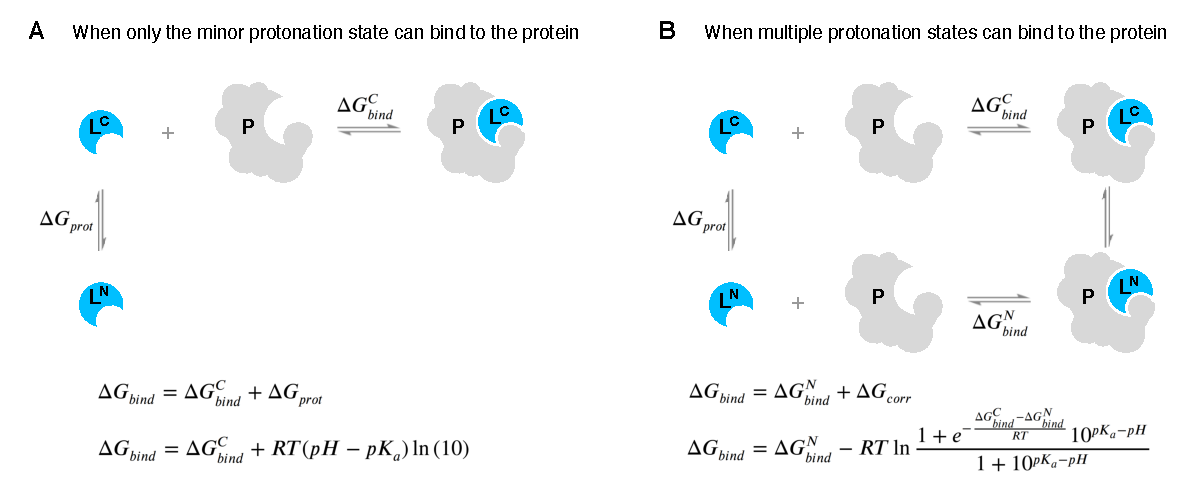
\includegraphics[width=1.0\linewidth]{figures/pKa-effects-on-protein-ligand-binding.pdf}
\caption{ {\bf Aqueous ligand \pKa{} can influence overall protein-ligand binding affinity.} 
{\bf A} When only the minor aqueous protonation state contributes to protein-ligand complex formation, the overall binding free energy ($\Delta G_{bind}$) needs to be calculated as the sum of binding affinity of the minor state and the protonation penalty of that state. 
{\bf B} When multiple charge states contribute to complex formation, the overall free energy of binding includes a multiple protonation states correction (MPSC) term ($\Delta G_{corr}$). 
MPSC is a function of pH, aqueous \pKa{} of the ligand, and the difference between the binding free energy of charged and neutral species ($\Delta G_{bind}^{C} - \Delta G_{bind}^{N}$).
}
\label{fig:pKa-effects-on-protein-ligand-binding}
\end{figure}

Using the equations in Fig.~\ref{fig:pKa-effects-on-protein-ligand-binding}B, we can model the true MPSC ($\Delta G_{corr}$) with respect to the difference between pH and the \pKa{} of the ligand to see when this value has a significant impact on the overall binding free energy. 
In Fig.~\ref{fig:pKa-inaccuracy-and-MPSC}, the true MPSC that must be added to $\Delta G_{bind}^{N}$ is shown for ligands with varying binding affinity difference between protonation states ($\Delta\Delta G = \Delta G_{bind}^{C} - \Delta G_{bind}^{N}$). Fig.~\ref{fig:pKa-inaccuracy-and-MPSC}A shows the case of a monoprotic base in which the charged state has a lower affinity than the neutral state. 
Solid lines depict the accurate correction value. 
In cases where the \pKa{} is lower than the pH, the correction factor disappears as the ligand fully populates the neutral state ($\Delta G_{bind} = \Delta G_{bind}^{N}$). 
As the pH dips below the \pKa{}, the charged state is increasingly populated and $\Delta G_{corr}$ increases to approach $\Delta\Delta G$. 

It is interesting to note the pH-\pKa{} range over which $\Delta G_{corr}$ changes significantly.
It is often assumed that, for a basic ligand, if the \pKa{} of a ligand is more than 2 units higher than the pH, only 1\% of the population is in the neutral state according to Henderson-Hasselbalch equation, and it is safe to approximate the overall binding affinity with $\Delta G_{bind}^{C}$. 
Based on the magnitude of the relative free energy difference between ligand protonation states, this assumption is not always correct. 
As seen in Fig.~\ref{fig:pKa-inaccuracy-and-MPSC}A, the responsive region of $\Delta G_{corr}$ can span 3 pH units for a system with $\Delta\Delta G = 1 kcal/mol$, or 5 pH units for a system with $\Delta\Delta G = 4 kcal/mol$. 
This highlights that the range of \pKa{} values that impact binding affinity predictions is wider than 2 pH units. 
Molecules with \pKa{}~ values several units away from the physiological pH can still impact the overall binding affinity significantly due to the MPSC. 

Despite the need to capture the contributions of multiple protonation states by including the MPSC in binding affinity calculations, inaccurate \pKa{} predictions can lead to errors in $\Delta G_{corr}$ and overall free energy of binding prediction. 
In Fig.~\ref{fig:pKa-inaccuracy-and-MPSC}A dashed lines show predicted $\Delta G_{corr}$ based on \pKa{} error of -1 units. 
We have chosen a \pKa{} error of 1 unit as this is the average inaccuracy expected from the \pKa{} prediction methods based on the SAMPL6 Challenge.
Underestimation of the \pKa{} causes the $\Delta G_{corr}$ to be underestimated as well and will result in overestimated affinities (i.e., too negative binding free energy) for a varying range of pH - \pKa{} values depending on the binding affinity difference between protonation states($\Delta\Delta G$).
In Fig.~\ref{fig:pKa-inaccuracy-and-MPSC}B dashed lines show how the magnitude of the absolute error caused by calculating $\Delta G_{corr}$ with an inaccurate \pKa{} varies with respect to pH. 
Different colored lines show simulated results with varying binding free energy differences between protonation states. 
For a system whose charged state has higher binding free energy than the neutral state ($\Delta\Delta G$ = 2 kcal/mol), the absolute error caused by underestimated \pKa{} by 1 unit can be up to 0.9 kcal/mol.
For a system whose charged state has an even lower affinity (more positive binding free energy) than the neutral state ($\Delta\Delta G$ = 4 kcal/mol), the absolute error caused by underestimated \pKa{} by 1 unit can be up to 1.2 kcal/mol.
The magnitude of errors contributing to overall binding affinity is too large to be neglected. Improving the accuracy of small molecule \pKa{} prediction methods can help to minimize the error in predicted MPSC.

With the current level of \pKa{} prediction accuracy as observed in SAMPL6 Challenge, is it advantageous to include the MPSC in affinity predictions that may include errors caused by \pKa{} predictions? 
We provide a comparison of the two choices to answer this question: (1) Neglecting the MPSC completely and assuming overall binding affinity is captured by $\Delta G_{bind}^{N}$, (2) including MPSC with a potential error in overall affinity calculation. 
The magnitude of error caused by Choice 1 (ignoring MPSC) is depicted as a solid line in Fig.~\ref{fig:pKa-inaccuracy-and-MPSC}B and the magnitude of error caused by MPSC computed with inaccurate \pKa{}  is depicted as dashed lines. 
What is the best strategy? 
Error due to choice 1 is always larger than error due to choice 2 for all pH-\pKa{} values. 
In this scenario, including the MPSC improves overall binding affinity prediction accuracy.
The error caused by the inaccurate \pKa{} is smaller than the error caused by neglecting the MPSC. 

We can also ask whether or not an MPSC calculated based on an inaccurate \pKa{} should be included in binding affinity predictions in different circumstances, such as underestimated or overestimated \pKa{} values and charged states with higher or lower affinities than the neutral states. 
We tried to capture these circumstances in four quadrants of Fig.~\ref{fig:pKa-inaccuracy-and-MPSC}. 
In the case of overestimated \pKa{} values (Fig.~\ref{fig:pKa-inaccuracy-and-MPSC}E-H), it can be seen that for most of the pH-\pKa{} range, it is more advantageous to include the predicted MPSC in affinity calculations, except a smaller window where the opposite choice would be more advantageous. 
For instance, for the system with $\Delta\Delta G$ = 2~kcal/mol and overestimated \pKa{} (Fig.~\ref{fig:pKa-inaccuracy-and-MPSC}E) for the pH-\pKa{} region between -0.5 and 2, including the predicted $\Delta G_{corr}$ introduces more error than ignoring the MPSC. 

In practice, we normally do not know the exact magnitude or the direction of the error of our predicted \pKa{}. 
Therefore, using simulated MPSC error plots to decide when to include MPSC in binding affinity predictions is not possible. 
However, based on the analysis of a case with 1 unit of \pKa{} error, including the MPSC correction would be more often than not helpful in improving binding affinity predictions. 
The detrimental effect of \pKa{} inaccuracy is still significant. 
Hopefully, future improvements in \pKa{} prediction methods will improve the accuracy of the MPSC and binding affinity predictions of ligands which have multiple protonation states that contribute to aqueous or complex populations. 
Being able to predict \pKa{}~ values with 0.5 units accuracy, for example, would significantly aid binding affinity models in computing more accurate MPSC terms.   

The whole analysis presented in this section assumes that at least the dominant protonation state of the ligand is correctly included in the modeling of the protein-ligand complex. 
We have not discussed the case of omitting this dominant state from the free energy calculations entirely when it is erroneously predicted to be a minor state in solution. 
Such a mistake could be the most problematic, and the errors in estimated binding free energy could be very large.

\begin{figure}
\centering
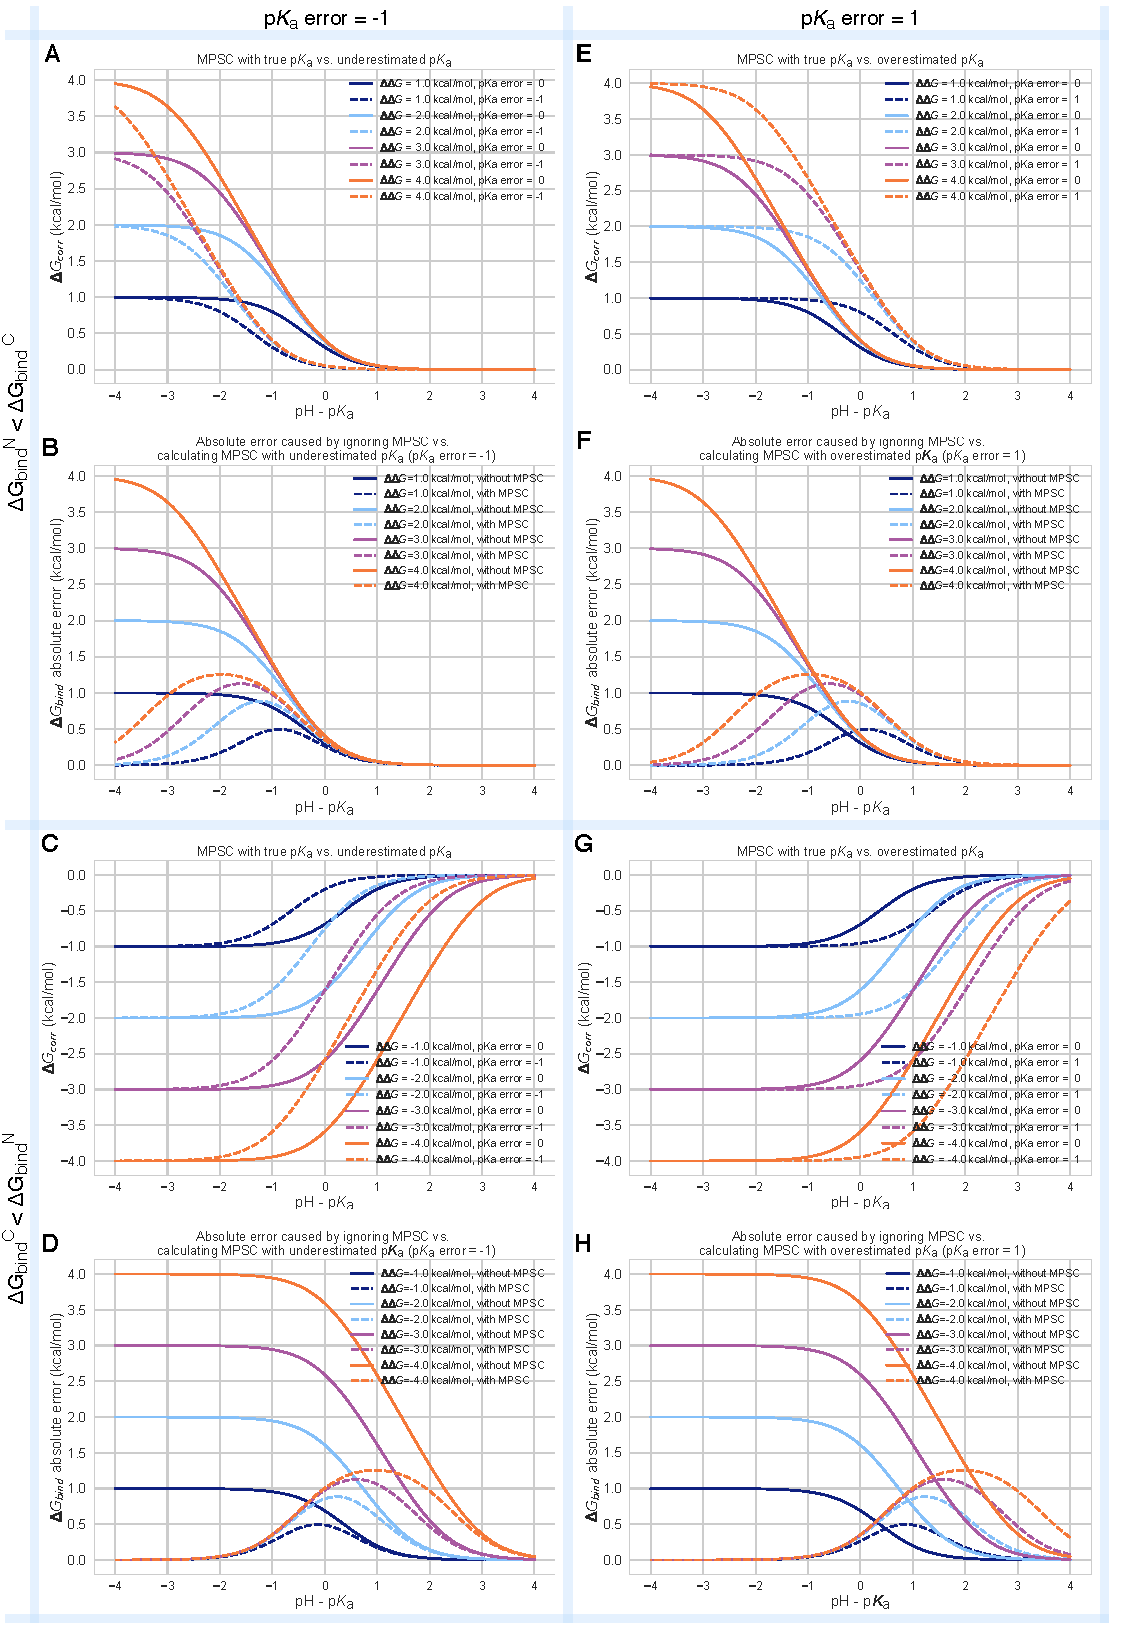
\includegraphics[width=0.8\linewidth]{figures/pKa-inaccuracy-and-MPSC.pdf}
\caption{ {\bf Inaccuracy of \pKa{} prediction ($\pm$ 1 unit) affects the the accuracy of MPSC and overall protein-ligand binding free energy calculations to varying degrees based on aqueous \pKa{} and relative binding affinity of individual protonation states ($\Delta\Delta G = \Delta G_{bind}^{C} - \Delta G_{bind}^{N}$).} 
All calculations are made for 25\degree C, and a ligand with a single basic titratable group. {\bf A, C, E, and G} show MPSC ($\Delta G_{corr}$) calculated with true vs. inaccurate \pKa{}. 
{\bf B, D, F, and H} show the comparison of the absolute error to $\Delta G_{bind}$ caused by ignoring the MPSC completely (solid lines) vs. calculating MPSC based in inaccurate \pKa{} value (dashed lines). 
These plots provide guidance on when it is beneficial to include MPSC correction based on \pKa{} error, pH - \pKa{}, and $\Delta\Delta G$. 
}
\label{fig:pKa-inaccuracy-and-MPSC}
\end{figure}



%%%
\subsection{Take-away lessons from SAMPL6 \pKa{} Challenge}

The SAMPL6 \pKa{} Challenge showed that, in general, \pKa{} prediction accuracy of computational methods is lower than expected for drug-like molecules. 
Our expectation prior to the blind challenge was that well-developed methods would achieve prediction errors as low was 0.5 \pKa{} units, and make reliable predictions of dominant charge and tautomer states in solution. 
There are many factors that complicate predicting \pKa{} values of drug-like molecules: multiple titratable sites, including tautomerization, frequent presence of heterocycles, and extended conjugation patterns, as well as high numbers of rotatable bonds and the possibility of intramolecular hydrogen bonds.
Macroscopic \pKa{} predictions have not yet reached experimental accuracy (where the inter-method variability of macroscopic \pKa{} measurements is around 0.5 \pKa{} units~\citep{Fraczkiewicz:2013:ReferenceModuleinChemistryMolecularSciencesandChemicalEngineering}). 
There was not a single method in the SAMPL6 Challenge that achieved RMSE around 0.5 or lower for macroscopic \pKa{} predictions for the 24 molecule set of kinase inhibitor fragment-like molecules.
Smaller RMSEs were observed in the microscopic \pKa{} evaluation section of this study for some methods; however, the 8 molecule set used for that analysis poses a very limited dataset to reach conclusions about general expectations for drug-like molecules.

As the majority of experimental data was in the form of macroscopic \pKa{} values, we had to adopt a numerical matching algorithm (Hungarian matching) to pair predicted and experimental values to calculate performance statistics of macroscopic \pKa{} predictions. 
Accuracy, correlation, and extra/missing \pKa{} prediction counts were the main metrics for macroscopic \pKa{} evaluations. 
An RMSE range of 0.7 to 3.2 \pKa{} units was observed for all methods.
Only five methods achieved RMSE between 0.7--1 \pKa{} units, while an RMSE between 1.5--3 log units was observed for the majority of methods. 
All four methods of the LFER category and three out of 5 QSPR/ML methods achieved RMSE less than 1.5 \pKa{} units.
All the QM methods that achieved this level of performance included linear empirical corrections to rescale and unbias their \pKa{} predictions. 

Based on the consideration of multiple error metrics, we compiled a shortlist of consistently-well performing methods for macroscopic \pKa{} evaluations. 
Two methods from QM+LEC methods, one QSPR/ML, two empirical methods achieved consistent performance according to many metrics. 
The common features of the two empirical methods were their large training sets (16000--17000 compounds) and commercial nature.

There were four submissions of QM-based methods that utilized the COSMO-RS implicit solvation model. 
While three of these achieved the lowest RMSE among QM-based methods (\textit{xvxzd}, \textit{yqkga}, and \textit{8xt50})~\citep{Pracht:2018:J.Comput.AidedMol.Des.}, one of them showed the highest RMSE (\textit{0hxtm} (COSMOtherm\_FINE17)). 
The comparison of these methods indicates that capturing the conformational ensemble of microstates, using high-level QM calculations, and including RRHO corrections contribute to better macroscopic \pKa{} predictions.
Linear empirical corrections applied QM calculations improved results, especially when the linear correction is calibrated for an experimental dataset using the same level of theory as the deprotonation free energy predictions (as in \textit{xvxzd}).
This challenge also points to the advantage of the COSMO-RS solvation approach compared to other implicit solvent models.

Molecules that posed greater difficulty for \pKa{} predictions were determined by comparing the macroscopic \pKa{} prediction accuracy of each molecule averaged over all methods submitted to the challenge. 
\pKa{} prediction errors were higher for compounds with sulfur-containing heterocycles, iodo, and bromo groups. 
This trend was also conserved when only QM-based methods were analyzed. 
The SAMPL6 \pKa{} dataset consisted of only 24 small molecules which limited our ability to statistically confirm this conclusion, however, we believe it is worth reporting molecular features that coincided with larger errors even if we can not evaluate the reason for these failures. 

Utilizing a numerical matching algorithm to pair experimental and predicted macroscopic \pKa{} values was a necessity, however, this approach did not capture all aspects of prediction errors. 
Computing the number of missing or extra \pKa{} predictions remaining after Hungarian matching provided a window for observing macroscopic \pKa{} prediction errors such as the number of macroscopic transitions or ionization states expected in a pH interval. 
In \pKa{} evaluation studies, it is typical to just focus on \pKa{} value errors evaluated after matching and to ignore \pKa{} prediction errors that the matching protocol can not capture~\citep{Balogh:2012:J.Pharm.Biomed.Anal.a, Settimo:2014:Pharm.Res.a, Meloun:2007:Anal.Bioanal.Chem., Liao:2009:J.Chem.Inf.Model., Manchester:2010:J.Chem.Inf.Model.}. 
Frequently ignored prediction errors include predicting missing or extra \pKa{}s and failing to predict the correct charge states. 
The SAMPL6 \pKa{} Challenge results showed sporadic presence of missing \pKa{} predictions and very frequent tendency to make extra \pKa{} predictions. 
Both indicate failures to capture the correct ionization states. 
The traditional way of evaluating \pKa{}s that only focuses on the \pKa{} value error after some sort of numerical match between predictions and experimental values may have motivated these types of errors as there would be no penalty for missing a macroscopic deprotonation and predicting an extra one. 
This problem does not seem to be specific to any method category.

We used the eight molecule subset of SAMPL6 compounds with NMR-based dominant microstate sequence information to demonstrate the advantage of evaluating \pKa{} prediction on the level of microstates.
Comparison of statistics computed for the 8 molecule dataset by Hungarian matching and microstate-based matching showed how Hungarian matching, despite being the best choice when only numerical matching is possible, can still mask errors in \pKa{} predictions. 
Errors computed by microstate-based matching were larger compared to numerical matching algorithms in terms of RMSE.
Microscopic \pKa{} analysis with numerical matching algorithms may mask errors due to the higher number of guesses made.
Numerical matching based on \pKa{} values also ignores information regarding the relative population of states. 
Therefore, it can lead to \pKa{}s defined between very low energy microstate pairs to be matched to the experimentally observable \pKa{} between microstates of higher populations. 
Of course, the predicted \pKa{} value could be correct however the predicted microstates would be wrong. 
Such mistakes caused by Hungarian matching were observed frequently in SAMPL6 results, and therefore we decided microstate-based matching of \pKa values provides a more realistic picture of method performance.  

Some QM and LFER methods made mistakes in predicting the dominant tautomers of the ionization states. 
Dominant tautomer prediction seemed to be particularly difficult for charged tautomers compared with neutral tautomers. 
The easiest way to extract the dominant microstate sequence from predictions was to calculate the relative free energy of microstates at any reference pH, determining the lowest free energy state in each ionization state.
Errors in dominant microstate predictions were very rare for neutral tautomers, but more frequent in cationic tautomers with +1 charge of the 8 molecule set. 
SM14 was the molecule with the lowest dominant microstate prediction accuracy, while dominant microstates predictions for SM15 were perfect for all molecules. 
SM14 and SM15 both possess two experimental \pKa{}s and a benzimidazole scaffold. 
The difference between them is the distance between the experimental \pKa{} values, which is smaller for SM14. 
These results make sense from the perspective of relative free energies of microstates. 
Closer \pKa{} values mean that the free energy difference between different microstates is smaller for SM14, and therefore any error in predicting the relative free energy of tautomers is more likely to cause reordering of relative populations of microstates and impact the accuracy of dominant microstate predictions. 
It would have been extremely informative to evaluate the tautomeric ratios and relative free energy predictions of microstates, however, the experimental data needed for this approach was not available. 
Tautomeric ratios could not be measured by the experimental methods available to us. 
Resolving tautomeric ratios would require extensive NMR measurements, but these measurements can suffer from lower accuracy especially when the free energy difference between tautomers is large.

%According to statistics calculated with microstate-based matching, we determined a shortlist of consistently well-performing methods for microscopic \pKa{} predictions of 8 molecule set. These methods that ranked in the top 10 according to RMSE, MEA, and had perfect dominant microstate prediction accuracy included three methods from QM+LEC category and three from QSPR/ML category. Simulations Plus \pKa{} prediction method was the only method that appeared to be consistently well-performing in both the assessment for macroscopic and microscopic \pKa{} prediction (\textit{gyuhx} and \textit{hdiyq}), although, due to the size of the experimental datasets evaluation of macroscopic \pKa{} prediction carried more weight in this performance assessment. Still microscopic \pKa{} evaluation can provide much more in-depth analysis and can be more informative about capturing reasons for failure.

The overall assessment of the SAMPL6 \pKa{} Challenge captured non-stellar performance for microscopic and macroscopic \pKa{} predictions which can be detrimental to the accuracy of protein-ligand affinity predictions and other pH-dependent physicochemical property predictions such as distribution coefficients, membrane permeability, and solubility.
Protein-ligand binding affinity predictions utilize \pKa{} predictions in two ways: determination of the relevant aqueous microstates and quantification of the free energy penalty to reach these states. 
More accurate microscopic \pKa{} predictions are needed to be able to accurately incorporate multiple protonation state corrections (MPSC) into overall binding affinity calculations. 

We simulated the effect of overestimating or underestimating \pKa{} of a ligand by one unit on overall binding affinity prediction for a ligand where both cation and neutral states contribute to binding affinity. 
A \pKa{} prediction error of this magnitude (assuming dominant tautomers were predicted correctly) could cause up to 0.9 and 1.2 kcal/mol error in overall binding affinity when the binding affinity of protonation states are 2 or 4 kcal/mol different, respectively. 
For the case of 4 kcal/mol binding affinity difference between protonation states, the pH-\pKa{} range that the error would be larger than 0.5 kcal/mol surprisingly spans around 3.5 pH units. 
The worse case, of course, is where there is a significant difference in binding free energy between the two protonation states, but we include the wrong one in our free energy calcuation.
We demonstrated that the range of pH-\pKa{} value that the MPSC needs to be incorporated in binding affinity predictions can be wider than the widely assumed range of 2 pH units, based on the affinity difference between protonation states. 
At the level of 1 unit \pKa{} error, incorporating the MPSC would improve binding affinity predictions more often than not. 
If the microscopic \pKa{} could be predicted with 0.5 \pKa{} units of accuracy, MPSC calculations would be much more reliable.

There are multiple factors to consider when deciding which \pKa{} prediction method to utilize. 
These factors include the accuracy of microscopic and macroscopic \pKa{} values, the accuracy of the number and the identity of ionization states predicted within the experimental pH interval, the accuracy of microstates predicted within the experimental pH interval, the accuracy of tautomeric ratio (i.e., relative free energy between microstates), how costly is the calculation in terms of time and resources, and whether one has access to software licenses that might be required. 

All of the top-performing empirical methods were developed as commercial software that requires a license to run, and there were not any open-source alternatives for empirical \pKa{} predictions. 
Since the completion of the blind challenge, two publications reported open-source machine learning-based \pKa{} prediction methods, however, one can only predict the most acidic or most basic macroscopic \pKa{} values of a molecule~\citep{Mansouri:2019:J.Cheminformatics} and the second one is only trained for predicting \pKa{} values of monoprotic molecules~\citep{Baltruschat:2020:F1000Research}. 
Recently, a \pKa{} prediction methodology was published that describes a mixed approach of semi-empirical QM calculations and machine learning that can predict macroscopic \pKa{}s of both mono- and polyprotic species~\citep{Hunt:2020:J.Chem.Inf.Model.}. 
The authors reported RMSE of 0.85 for the retrospective analysis performed on the SAMPL6 dataset.



%%%
\subsection{Suggestions for future blind challenge design and evaluation of \pKa{} predictions}

This analysis helped us understand the current state of the field and led to many lessons informing future SAMPL challenges. 
We believe the greatest benefit can be achieved if further iterations of small molecule \pKa{} prediction challenges can be organized, creating motivation for improving protonation state prediction methods for drug-like molecules. 
In future challenges, it is desirable to increase chemical diversity to cover more common scaffolds~\citep{Zdrazil:2018:J.Med.Chem.} and functional groups~\citep{Ertl:2020:J.Med.Chem.} seen in drug-like molecules, gradually increasing the complexity of molecules.

\paragraph{Microscopic \pKa{} measurements are needed for careful benchmarking of \pKa{} predictions for multiprotic molecules.}
Future challenges should promote stringent evaluation for \pKa{} prediction methods from the perspective of microscopic \pKa{} and microstate predictions.
It is necessary to assess the capability of \pKa{} prediction methods to capture the free energy profile of microstates of multiprotic molecules. 
This is critical because \pKa{} predictions are often utilized to determine relevant protonation states and tautomers of small molecules that must be captured in other physical modeling approaches, such as protein-ligand binding affinity or distribution coefficient predictions. 
Different tautomers can have different binding affinities and partition coefficients.

In this paper, we demonstrated how experimental microstate information can guide the analysis further than the typical \pKa{} evaluation approach that has been used so far. 
The traditional \pKa{} evaluation approach focuses solely on the numerical error of the \pKa{} values and neglects the difference between macroscopic and microscopic \pKa{} definitions.
This is mainly caused by the lack of \pKa{} datasets with microscopic detail. 
To improve \pKa{} and protonation state predictions for multiprotic molecules, it is necessary to embrace the difference between macroscopic and microscopic \pKa{} definitions and select strategies for experimental data collection and prediction evaluation accordingly.
In the SAMPL6 Challenge, the analysis was limited by the availability of experimental microscopic data as well. 
As is usually the case, macroscopic \pKa{} values were abundant (24 molecules) and limited data on microscopic states was available (8 molecules), although the latter opened new avenues for evaluation. 
For future blind challenges for multiprotic compounds, striving to collect experimental datasets with microscopic \pKa{}s would be very beneficial, despite the high cost of these measurements. 
Benchmark datasets of microscopic \pKa{}~ values with assigned microstates are currently missing because experimental determination of these are much more expensive and time-consuming than macroscopic \pKa{} measurements. 
This limits the ability to improve \pKa{} and tautomer prediction methods for multiprotic molecules. 
If the collection of experimental microscopic \pKa{}s is not possible due to time and resource costs of such NMR experiments, at least supplementing the more automated macroscopic \pKa{} measurements with NMR-based determination of the dominant microstate sequence or tautomeric ratios of each ionization state can create very useful benchmark datasets. 
This supplementary information can allow microstate-based assignment of experimental to predicted \pKa{}~ values and a more realistic assessment of method performance.

\paragraph{Evaluation strategy for \pKa{} predictions must be determined based on the nature of experimental \pKa{} measurements available.}
If the only available experimental data is in the form of macroscopic \pKa{} values, the best way to evaluate computational predictions is by calculating predicted macroscopic \pKa{} from microscopic \pKa{} predictions. 
With the conversion of microscopic \pKa{} to macroscopic \pKa{}s, all structural information about the titration site is lost, and the only remaining information is the total charge of macroscopic ionization states.
Unfortunately, most macroscopic \pKa{} measurements---including potentiometric and spectrophotometric methods---do not capture the absolute charge of the macrostates. 
The spectrophotometric method does not measure charge at all. 
The potentiometric method can only capture the relative charge changes between macrostates.  
Only pH-dependent solubility-based \pKa{} estimations can differentiate neutral and charged states from one another. 
It is, therefore, very common to have experimental datasets of macroscopic \pKa{} without any charge or protonation position information regarding the macrostates.
This causes an issue of assigning predicted and experimental \pKa{} values before any error statistics can be calculated.

As delineated by Fraczkiewicz ~\citep{Fraczkiewicz:2013:ReferenceModuleinChemistryMolecularSciencesandChemicalEngineering}, the fairest and most reasonable solution for the \pKa{} matching problem involves an assignment algorithm that preserves the order of predicted and experimental microstates and uses the principle of smallest differences to pair values. 
We recommend Hungarian matching with a squared-error penalty function. 
The algorithm is available in SciPy package (scipy.optimize.linear\_sum\_assignment)~\citep{SciPy-linear-sum-assignment}.
In addition to the analysis of numerical error statistics following Hungarian matching, at the very least, the number of missing and extra \pKa{} predictions must be reported based on unmatched \pKa{} values. 
Missing or extra \pKa{} predictions point to a problem with capturing the right number of ionization states within the pH interval of the experimental measurements. 
We have demonstrated that for microscopic \pKa{} predictions, performance analysis based on Hungarian matching results in overly optimistic and misleading results---instead the employed microstate-based matching provided a more realistic assessment when microstate data is available. 

\paragraph{Lessons from the first \pKa{} blind challenge will guide future decisions on challenge rules, prediction reporting formats, and challenge inputs.}
We solicited three different submission types in SAMPL6 to capture all the necessary information related to \pKa{} predictions. 
These were (1) macroscopic \pKa{} values, (2) microscopic \pKa{} values and microstate pair identities, and (3) fractional population of microstates with respect to pH. 
We realized later that collecting fractional populations of microstates was redundant since microscopic \pKa{} values and microstate pairs capture all the necessary information to construct fractional population vs. pH curves ~\citep{Gunner:2020:J.Comput.AidedMol.Des.}.  
Only microscopic and macroscopic \pKa{} values were used for the challenge analysis presented in this paper.

While exploring ways to evaluate SAMPL6 \pKa{} Challenge results, we developed a better way to capture microscopic \pKa{} predictions, as presented in \citet{Gunner:2020:J.Comput.AidedMol.Des.}. 
This alternative reporting format consists of reporting the charge and relative free energy of microstates with respect to an arbitrary reference microstate and pH.
This approach presents the most concise method of capturing all necessary information regarding microscopic \pKa{} predictions and allows calculation of predicted microscopic \pKa{}s, microstate population with respect to pH, macroscopic \pKa{}~ values, macroscopic population with respect to pH, and tautomer ratios. 
Still, there may be methods developed to predict macroscopic \pKa{}s directly instead of computing them from microstate predictions that justifies allowing a macroscopic \pKa{} reporting format. 
In future challenges, we recommend collecting \pKa{} predictions with two submission types: (1) macroscopic \pKa{} values together with the charges of the macrostates and (2) microstates, their total charge, and relative free energies with respect to a specified reference microstate and pH. 
This approach is being used in SAMPL7.

In SAMPL6, we provided an enumerated list of microstates and their assigned microstate IDs because we were worried about parsing submitted microstates in SMILES from different sources correctly. 
There were two disadvantages to this approach. 
First, this list of enumerated microstates was used as input by some participants which was not our intention. (Challenge instructions requested that predictions should not rely on these microstate lists and only use them for matching microstate IDs.) 
Second, the first iteration of enumerated microstates was not complete. 
We had to add new microstates and assign them microstate IDs for a couple of rounds until reaching a complete list. 
In future challenges, a better way of handling the problem of capturing predicted microstates would be asking participants to specify the predicted protonation states themselves and assigning identifiers after the challenge deadline to aid comparative analysis. 
This would prevent the partial unblinding of protonation states and allow the assessment of whether methods can predict all the relevant states independently, without relying on a provided list of microstates.
Predicted states can be submitted as mol2 files that represent the microstate with explicit hydrogens. 
The organizers must only provide the microstate that was selected as the reference state for the relative microstate free energy calculations. 


In the SAMPL6 \pKa{} Challenge, there was not a requirement that participants should report predictions for all compounds. 
Some participants reported predictions for only a subset of compounds, which may have led these methods to look more accurate than others due to missing predictions.
In the future, it will be better to allow submissions of only complete sets for a better comparison of method performance. 

A wide range of methods participated in the SAMPL6 \pKa{} Challenge---from very fast QSPR methods to QM methods with a high-level of theory and extensive exploration of conformational ensembles. 
In the future, it would be interesting to capture computing costs in terms of average compute hours per molecule. 
This can provide guidance to future users of \pKa{} prediction methods for selection of which method to use.

Some molecules suffered from less accurate \pKa{} predictions than others in SAMPL6.  To understand the reason for these failures better, it can be helpful to ask participants who submit empirical prediction methods to inspect their training sets for the presence of similar compounds and optionally report it.  


\paragraph{It is advantageous to field associated challenges with common set of molecules for different physicochemical properties.}
Future blind challenges can maximize learning opportunities by evaluating predictions of different physicochemical properties for the same molecules in consecutive challenges. 
In SAMPL6, we organized both \pKa{} and \logP{} challenges. 
Unfortunately only a subset of compounds in the \pKa{} datasets were suitable for the potentiometric \logP{} measurements~\cite{Isik:2018:J.Comput.AidedMol.Des.}. 
Still, comparing prediction performance of common compounds in both challenges can lead to beneficial insights especially for physical modeling techniques if there are common aspects that are beneficial or detrimental to prediction performance. 
For example, in SAMPL6 \pKa{} and \logP{} Challenges COSMO-RS and EC-RISM solvation models achieved good performance.
Having access to a variety of physicochemical property measurements can also help the identification of error sources.
For example, dominant microstates determined for \pKa{} challenge can provide information to check if correct tautomers are modeling in a \logP{} or \logD{} challenge.
\pKa{} prediction is a requirement for \logD{} prediction and experimental \pKa{} values can help diagnosing the source of errors in \logD{} predictions better. 
The physical challenges in SAMPL7, for which the blind portion of the challenges have just concluded on October 8th, 2020, follow this principle and include both \pKa{}, \logP{}, and membrane permeability properties for a set of monoprotic compounds. 
We hope that future \pKa{} challenges can focus on multiprotic drug-like compounds with microscopic \pKa{} measurements for an in-depth analysis.



%%%%%%%%%%%%%%%%%%%%%%%%%%%%%%%%%%%%%%%%%%%%%%%%%%%%%%%%%%%%
% Conclusion
%%%%%%%%%%%%%%%%%%%%%%%%%%%%%%%%%%%%%%%%%%%%%%%%%%%%%%%%%%%%
\section{Conclusion}

The first SAMPL6 \pKa{} Challenge focused on molecules resembling fragments of kinase inhibitors, and was intended to assess the performance of \pKa{} predictions for drug-like molecules. 
With wide participation, we had an opportunity to prospectively evaluate \pKa{} predictions spanning various empirical and QM based approaches. 
In addition to community participants, a small number of popular \pKa{} prediction methods that were missing from blind submissions were added as reference calculations after the challenge deadline. 

Practical experimental limitations restricted the overall size and microscopic information available for the blind challenge dataset~\cite{Isik:2018:J.Comput.AidedMol.Des.}.
The experimental dataset consisted of spectrophotometric measurements of 24 molecules, some of which were multiprotic. 
For a subset of molecules there was also NMR data to inform the dominant microstate sequence, though microscopic \pKa{} measurements were not performed. 
We conducted a comparative analysis of methods represented in the blind challenge in terms of both macroscopic and microscopic \pKa{} prediction performance avoiding any assumptions about the interpretation of experimental \pKa{}s. 

Here, we used Hungarian matching to assign predicted and experimental values for the calculation of accuracy and correlation statistics, because the majority of experimental data was macroscopic \pKa{} values. 
In addition to evaluating error in predicted \pKa{} values, we also reported the macroscopic \pKa{} errors that were not captured by the match between experimental and predicted \pKa{} values. 
These were extra or missing \pKa{} predictions which are important indicators that predictions are failing to capture the correct ionization states. 

We evaluated microscopic \pKa{} predictions utilizing the experimental dominant microstate sequence data of eight molecules. 
This experimental data allowed us to use microstate-based matching for evaluating the accuracy of microscopic \pKa{} values in a more realistic way. 
We have determined that QM and LFER predictions had lower accuracy in determining the dominant tautomer of the charged microstates than the neutral states. 
For both macroscopic and microscopic \pKa{} predictions we have determined methods that were consistently well-performing according to multiple statistical metrics. 
Focusing on the comparison of molecules instead of methods for macroscopic \pKa{} prediction accuracy indicated molecules with sulfur-containing heterocycles, iodo, and bromo groups suffered from lower \pKa{} prediction accuracy. 

The overall performance of \pKa{} predictions as captured in this challenge is concerning for the application of \pKa{} prediction methods in computer-aided drug design. 
Many computational methods for predicting target affinities and physicochemical properties rely on \pKa{} predictions for determining relevant protonation states and the free energy penalty of such states. 
1 unit of \pKa error is an optimistic estimate of current macroscopic \pKa{} predictions for drug-like molecules based on SAMPL6 Challenge where errors in predicting the correct number of ionization states or determining the correct dominant microstate were also common to many methods.
In the absence of other sources of errors, we showed that 1 unit over- or underestimation of the \pKa{} of a ligand can cause significant errors in the overall binding affinity calculation due to errors in multiple protonation state correction factor. 

The SAMPL6 GitHub Repository contains all information regarding the challenge structure, experimental data, blind prediction submission sets, and evaluation of methods. 
The repository will be useful for future follow up analysis and the experimental measurements can continue to serve as a benchmark dataset for testing methods. 

In this article, we aimed to demonstrate not only the comparative analysis of the \pKa{} prediction performance of contemporary methods for drug-like molecules, but also to propose a stringent \pKa{} prediction evaluation strategy that takes into account differences in microscopic and macroscopic \pKa{} definitions. We hope that this study will guide and motivate further improvement of \pKa{} prediction methods.



%%%%%%%%%%%%%%%%%%%%%%%%%%%%%%%%%%%%%%%%%%%%%%%%%%%%%%%%%%%%
% Code and Data Availability
%%%%%%%%%%%%%%%%%%%%%%%%%%%%%%%%%%%%%%%%%%%%%%%%%%%%%%%%%%%%
\section{Code and data availability} \label{Code-and-Data-Availability}
\begin{minipage}{15cm}
\begin{itemize}

\item SAMPL6 \pKa{} challenge instructions, submissions, experimental data and analysis is available at SAMPL6 GitHub Repository: \href{https://github.com/samplchallenges/SAMPL6}{https://github.com/samplchallenges/SAMPL6}

\end{itemize}
\end{minipage}


%%%%%%%%%%%%%%%%%%%%%%%%%%%%%%%%%%%%%%%%%%%%%%%%%%%%%%%%%%%%
% Overview of supplementary information
%%%%%%%%%%%%%%%%%%%%%%%%%%%%%%%%%%%%%%%%%%%%%%%%%%%%%%%%%%%%
\section{Overview of supplementary information}

\paragraph{Contents of the Supplementary Information:}

\begin{itemize}
\item TABLE~\ref{pKa_chemical_identifiers_table}: SMILES and InChI identifiers of SAMPL6 \pKa{}  Challenge molecules.
\item TABLE~\ref{SI_statistics_table_macro_pKa}: Evaluation statistics calculated for all macroscopic \pKa{} prediction submissions based on Hungarian match for 24 molecules.
\item TABLE~\ref{SI-statistics-table-micro-pKa-8mol-hungarian}: Evaluation statistics calculated for all microscopic \pKa{} prediction submissions based on Hungarian match for 8 molecules with NMR data.
\item TABLE~\ref{SI-statistics-table-micro-pKa-8mol-microstate}: Evaluation statistics calculated for all microscopic \pKa{} prediction submissions based on microstate match for 8 molecules with NMR data.
\item FIGURE~\ref{fig:experimental-microstate-IDs-SI-table}: Dominant microstates of 8 molecules were determined based on NMR measurements.
\item FIGURE~\ref{fig:molecular_properties_vs_MAE_correlation}: MAE of macroscopic \pKa{} predictions of each molecule did not show any significant correlation with any molecular descriptor.
\item FIGURE~\ref{fig:macroscopic-pKa-error-vs-pKa-value}: The value of macroscopic \pKa{} was not a factor affecting prediction error seen in SAMPL6 Challenge according to the analysis with Hungarian matching.
\item FIGURE~\ref{fig:microstate-pairs-with-Hungarian-match-vs-experiments}: There was low agreement between experimental dominant microstate pairs and the predicted microstate pairs selected by Hungarian algorithm for microscopic \pKa{} predictions. 




\end{itemize}

\paragraph{Extra files included in \textit{supplementary-documents.tar.gz}:}  
\begin{itemize}
\item An archive copy of the \pKa{} Challenge directory of SAMPL6 GitHub Repository (\textit{SAMPL6-repository-pKa-directory.zip}) 
\item Table~\ref{pKa_chemical_identifiers_table} in CSV format (\textit{SAMPL6-pKa-chemical-identifiers-table.csv}) 
\item Table~\ref{SI_statistics_table_macro_pKa} in CSV format (\textit{macroscopic-pKa-statistics-24mol-hungarian-match.csv})
\item Table~\ref{SI-statistics-table-micro-pKa-8mol-hungarian} in CSV format (\textit{microscopic-pKa-statistics-8mol-hungarian-match-table.csv})
\item Table~\ref{SI-statistics-table-micro-pKa-8mol-microstate} in CSV format (\textit{microscopic-pKa-statistics-8mol-microstate-match-table.csv})
\item Figure~\ref{fig:experimental-microstate-IDs-SI-table} in CSV format (\textit{experimental-microstates-of-8mol-based-on-NMR.csv})
\item The Jupyter Notebook used for the enumeration of microstates (\textit{enumerate-microstates-with-Epik-and-OpenEye-QUACPAC.ipynb})
\item A CSV table of SAMPL6 molecule IDs and OpenEye OEChem generated SMILES (\textit{molecule\_ID\_and\_SMILES.csv})

\end{itemize}


%%%%%%%%%%%%%%%%%%%%%%%%%%%%%%%%%%%%%%%%%%%%%%%%%%%%%%%%%%%%
% Author Contributions 
%%%%%%%%%%%%%%%%%%%%%%%%%%%%%%%%%%%%%%%%%%%%%%%%%%%%%%%%%%%%
\section{Author Contributions}

Conceptualization, MI, JDC ; Methodology, MI, JDC, ASR ; Software, MI, AR, ASR ; Formal Analysis, MI, ASR ; Investigation, MI ; Resources, JDC, DLM;  Data Curation, MI ; Writing-Original Draft, MI; Writing - Review and Editing, MI, JDC, ASR, AR, DLM, MRG; Visualization, MI, AR ; Supervision, JDC, DLM ; Project Administration, MI ; Funding Acquisition, JDC, DLM, MI.

%(Follow the \href{http://www.cell.com/pb/assets/raw/shared/guidelines/CRediT-taxonomy.pdf}{CRediT Taxonomy})

%%%%%%%%%%%%%%%%%%%%%%%%%%%%%%%%%%%%%%%%%%%%%%%%%%%%%%%%%%%%
% Acknowledgments 
%%%%%%%%%%%%%%%%%%%%%%%%%%%%%%%%%%%%%%%%%%%%%%%%%%%%%%%%%%%%
\section{Acknowledgments}

We would like to acknowledge the infrastructure and website support of Mike Chiu that allowed a seamless collection of challenge submissions. 
Mike Chiu also provided assistance with constructing a submission validation script to ensure all submissions adhered to the machine-readable format. 
We are grateful to Kiril Lanevskij for suggesting the Hungarian algorithm for matching experimental and predicted \pKa{} values. 
We would like to thank Thomas Fox for providing MoKa reference calculations.
We acknowledge Caitlin Bannan for guidance on defining a working microstate definition for the challenge and guidance for designing the challenge. 
We thank Brad Sherborne for his valuable insights at the conception of the \pKa{} challenge and connecting us with Timothy Rhodes and Dorothy Levorse who were able to provide resources and expertise for experimental measurements performed at MRL. 
We acknowledge Paul Czodrowski who provided feedback on multiple stages of this work: challenge construction, purchasable compound selection, and manuscript draft. 
MI, JDC, and DLM gratefully acknowledge support from NIH grant R01GM124270 supporting the SAMPL Blind Challenges.
MI, ASR, AR, and JDC acknowledge support from the Sloan Kettering Institute.
JDC acknowledges support from NIH grant P30CA008748 and NIH grant R01GM121505. 
DLM appreciates financial support from the National Institutes of Health (R01GM108889) and the National Science Foundation (CHE 1352608).
MRG acknowledges support of MCB-1519640 from the National Science Foundation. 
MI acknowledges Doris J.\ Hutchinson Fellowship. 
MI, ASR, AR, and JDC are grateful to OpenEye Scientific for providing a free academic software license for use in this work.
MI, ASR, AR, and JDC thank Janos Fejervari and ChemAxon team that gave us permission to include ChemAxon/Chemicalize \pKa{} predictions as a reference prediction in challenge analysis. 


%%%%%%%%%%%%%%%%%%%%%%%%%%%%%%%%%%%%%%%%%%%%%%%%%%%%%%%%%%%%
% Disclaimers
%%%%%%%%%%%%%%%%%%%%%%%%%%%%%%%%%%%%%%%%%%%%%%%%%%%%%%%%%%%%
\section{Disclaimers}

The content is solely the responsibility of the authors and does not necessarily represent the official views of the National Institutes of Health.

%%%%%%%%%%%%%%%%%%%%%%%%%%%%%%%%%%%%%%%%%%%%%%%%%%%%%%%%%%%%
% Disclosures 
%%%%%%%%%%%%%%%%%%%%%%%%%%%%%%%%%%%%%%%%%%%%%%%%%%%%%%%%%%%%
\section{Disclosures}

JDC was a member of the Scientific Advisory Board for Schr\"{o}dinger, LLC during part of this study, and is a current Scientific Advisory Board member for OpenEye Scientific and scientific advisor to Foresite Labs.
DLM is a current member of the Scientific Advisory Board of OpenEye Scientific and an Open Science Fellow with Silicon Therapeutics.

The Chodera laboratory receives or has received funding from multiple sources, including the National Institutes of Health, the National Science Foundation, the Parker Institute for Cancer Immunotherapy, Relay Therapeutics, Entasis Therapeutics, Vir Biotechnology, Silicon Therapeutics, EMD Serono (Merck KGaA), AstraZeneca, Vir Biotechnology, XtalPi, the Molecular Sciences Software Institute, the Starr Cancer Consortium, the Open Force Field Consortium, Cycle for Survival, a Louis V. Gerstner Young Investigator Award, The Einstein Foundation, and the Sloan Kettering Institute.
A complete list of funding can be found at \url{http://choderalab.org/funding}.

%%%%%%%%%%%%%%%%%%%%%%%%%%%%%%%%%%%%%%%%%%%%%%%%%%%%%%%%%%%%
%%% BIBLIOGRAPHY
%%%%%%%%%%%%%%%%%%%%%%%%%%%%%%%%%%%%%%%%%%%%%%%%%%%%%%%%%%%%


%\nocite{*} % This command displays all refs in the bib file. PLEASE DELETE IT BEFORE YOU SUBMIT YOUR MANUSCRIPT!
\bibliography{zotero, manual}


%%%%%%%%%%%%%%%%%%%%%%%%%%%%%%%%%%%%%%%%%%%%%%%%%%%%%%%%%%%%
% Supplementary Information
%%%%%%%%%%%%%%%%%%%%%%%%%%%%%%%%%%%%%%%%%%%%%%%%%%%%%%%%%%%%
\newpage
\beginsupplement
\section{Supplementary Information}



\begin{table}[]
\begin{center}
\begin{threeparttable}
\centering\scriptsize
\caption{{\bf SMILES and InChI identifiers of SAMPL6 \pKa{}  Challenge molecules.} A CSV version of this table can be found in \textit{SAMPL6-supplementary-documents.tar.gz}. SMILES were generated by OpenEye OEChem~\citep{oechem_openeye_2017}
} 
\centering\scriptsize
\label{pKa_chemical_identifiers_table}
\begin{tabular}{@{}lll@{}}
\toprule
SAMPL6 Molecule ID & Isomeric SMILES & InChI \\ \midrule
\rowcolor[HTML]{EFEFEF} 
SM01 & c1cc2c(cc1O)c3c(o2)C(=O)NCCC3 & \begin{tabular}[c]{@{}l@{}}InChI=1S/C12H11NO3/c14-7-3-4-10-9(6-7)8-2-1-5-13-12(15)11(8)16-10/\\ h3-4,6,14H,1-2,5H2,(H,13,15)\end{tabular} \\
SM02 & c1ccc2c(c1)c(ncn2)Nc3cccc(c3)C(F)(F)F & \begin{tabular}[c]{@{}l@{}}InChI=1S/C15H10F3N3/c16-15(17,18)10-4-3-5-11(8-10)21-14-12-6-1-2-7\\ -13(12)19-9-20-14/h1-9H,(H,19,20,21)\end{tabular} \\
\rowcolor[HTML]{EFEFEF} 
SM03 & c1ccc(cc1)Cc2nnc(s2)NC(=O)c3cccs3 & \begin{tabular}[c]{@{}l@{}}InChI=1S/C14H11N3OS2/c18-13(11-7-4-8-19-11)15-14-17-16-12(20-14)9\\ -10-5-2-1-3-6-10/h1-8H,9H2,(H,15,17,18)\end{tabular} \\
SM04 & c1ccc2c(c1)c(ncn2)NCc3ccc(cc3)Cl & \begin{tabular}[c]{@{}l@{}}InChI=1S/C15H12ClN3/c16-12-7-5-11(6-8-12)9-17-15-13-3-1-2-4-14(13)1\\ 8-10-19-15/h1-8,10H,9H2,(H,17,18,19)\end{tabular} \\
\rowcolor[HTML]{EFEFEF} 
SM05 & c1ccc(c(c1)NC(=O)c2ccc(o2)Cl)N3CCCCC3 & \begin{tabular}[c]{@{}l@{}}InChI=1S/C16H17ClN2O2/c17-15-9-8-14(21-15)16(20)18-12-6-2-3-7-13(1\\ 2)19-10-4-1-5-11-19/h2-3,6-9H,1,4-5,10-11H2,(H,18,20)\end{tabular} \\
SM06 & c1cc2cccnc2c(c1)NC(=O)c3cc(cnc3)Br & \begin{tabular}[c]{@{}l@{}}InChI=1S/C15H10BrN3O/c16-12-7-11(8-17-9-12)15(20)19-13-5-1-3-10-4-2\\ -6-18-14(10)13/h1-9H,(H,19,20)\end{tabular} \\
\rowcolor[HTML]{EFEFEF} 
SM07 & c1ccc(cc1)CNc2c3ccccc3ncn2 & \begin{tabular}[c]{@{}l@{}}InChI=1S/C15H13N3/c1-2-6-12(7-3-1)10-16-15-13-8-4-5-9-14(13)17-11-18\\ -15/h1-9,11H,10H2,(H,16,17,18)\end{tabular} \\
SM08 & Cc1ccc2c(c1)c(c(c(=O)[nH]2)CC(=O)O)c3ccccc3 & \begin{tabular}[c]{@{}l@{}}InChI=1S/C18H15NO3/c1-11-7-8-15-13(9-11)17(12-5-3-2-4-6-12)14(10-16\\ (20)21)18(22)19-15/h2-9H,10H2,1H3,(H,19,22)(H,20,21)\end{tabular} \\
\rowcolor[HTML]{EFEFEF} 
SM09 & COc1cccc(c1)Nc2c3ccccc3ncn2.Cl & \begin{tabular}[c]{@{}l@{}}InChI=1S/C15H13N3O.ClH/c1-19-12-6-4-5-11(9-12)18-15-13-7-2-3-8-14(1\\ 3)16-10-17-15;/h2-10H,1H3,(H,16,17,18);1H\end{tabular} \\
SM10 & c1ccc(cc1)C(=O)NCC(=O)Nc2nc3ccccc3s2 & \begin{tabular}[c]{@{}l@{}}InChI=1S/C16H13N3O2S/c20-14(10-17-15(21)11-6-2-1-3-7-11)19-16-18-1\\ 2-8-4-5-9-13(12)22-16/h1-9H,10H2,(H,17,21)(H,18,19,20)\end{tabular} \\
\rowcolor[HTML]{EFEFEF} 
SM11 & c1ccc(cc1)n2c3c(cn2)c(ncn3)N & \begin{tabular}[c]{@{}l@{}}InChI=1S/C11H9N5/c12-10-9-6-15-16(11(9)14-7-13-10)8-4-2-1-3-5-8/h1-7\\ H,(H2,12,13,14)\end{tabular} \\
SM12 & c1ccc2c(c1)c(ncn2)Nc3cccc(c3)Cl.Cl & \begin{tabular}[c]{@{}l@{}}InChI=1S/C14H10ClN3.ClH/c15-10-4-3-5-11(8-10)18-14-12-6-1-2-7-13(12)\\ 16-9-17-14;/h1-9H,(H,16,17,18);1H\end{tabular} \\
\rowcolor[HTML]{EFEFEF} 
SM13 & Cc1cccc(c1)Nc2c3cc(c(cc3ncn2)OC)OC & \begin{tabular}[c]{@{}l@{}}InChI=1S/C17H17N3O2/c1-11-5-4-6-12(7-11)20-17-13-8-15(21-2)16(22-3)9\\ -14(13)18-10-19-17/h4-10H,1-3H3,(H,18,19,20)\end{tabular} \\
SM14 & c1ccc(cc1)n2cnc3c2ccc(c3)N & \begin{tabular}[c]{@{}l@{}}InChI=1S/C13H11N3/c14-10-6-7-13-12(8-10)15-9-16(13)11-4-2-1-3-5-11/h1\\ -9H,14H2\end{tabular} \\
\rowcolor[HTML]{EFEFEF} 
SM15 & c1ccc2c(c1)ncn2c3ccc(cc3)O & \begin{tabular}[c]{@{}l@{}}InChI=1S/C13H10N2O/c16-11-7-5-10(6-8-11)15-9-14-12-3-1-2-4-13(12)15/\\ h1-9,16H\end{tabular} \\
SM16 & c1cc(c(c(c1)Cl)C(=O)Nc2ccncc2)Cl & \begin{tabular}[c]{@{}l@{}}InChI=1S/C12H8Cl2N2O/c13-9-2-1-3-10(14)11(9)12(17)16-8-4-6-15-7-5-8/\\ h1-7H,(H,15,16,17)\end{tabular} \\
\rowcolor[HTML]{EFEFEF} 
SM17 & c1ccc(cc1)CSc2nnc(o2)c3ccncc3 & \begin{tabular}[c]{@{}l@{}}InChI=1S/C14H11N3OS/c1-2-4-11(5-3-1)10-19-14-17-16-13(18-14)12-6-8-\\ 15-9-7-12/h1-9H,10H2\end{tabular} \\
SM18 & c1ccc2c(c1)c(=O)[nH]c(n2)CCC(=O)Nc3ncc(s3)Cc4ccc(c(c4)F)F & \begin{tabular}[c]{@{}l@{}}InChI=1S/C21H16F2N4O2S/c22-15-6-5-12(10-16(15)23)9-13-11-24-21(30\\ -13)27-19(28)8-7-18-25-17-4-2-1-3-14(17)20(29)26-18/h1-6,10-11H,7-9H2,\\ (H,24,27,28)(H,25,26,29)\end{tabular} \\
\rowcolor[HTML]{EFEFEF} 
SM19 & CCOc1ccc2c(c1)sc(n2)NC(=O)Cc3ccc(c(c3)Cl)Cl & \begin{tabular}[c]{@{}l@{}}InChI=1S/C17H14Cl2N2O2S/c1-2-23-11-4-6-14-15(9-11)24-17(20-14)21-1\\ 6(22)8-10-3-5-12(18)13(19)7-10/h3-7,9H,2,8H2,1H3,(H,20,21,22)\end{tabular} \\
SM20 & c1cc(cc(c1)OCc2ccc(cc2Cl)Cl)/C=C/3\textbackslash{}C(=O)NC(=O)S3 & \begin{tabular}[c]{@{}l@{}}InChI=1S/C17H11Cl2NO3S/c18-12-5-4-11(14(19)8-12)9-23-13-3-1-2-10(6-\\ 13)7-15-16(21)20-17(22)24-15/h1-8H,9H2,(H,20,21,22)/b15-7+\end{tabular} \\
\rowcolor[HTML]{EFEFEF} 
SM21 & c1cc(cc(c1)Br)Nc2c(cnc(n2)Nc3cccc(c3)Br)F & \begin{tabular}[c]{@{}l@{}}InChI=1S/C16H11Br2FN4/c17-10-3-1-5-12(7-10)21-15-14(19)9-20-16(23-\\ 15)22-13-6-2-4-11(18)8-13/h1-9H,(H2,20,21,22,23)\end{tabular} \\
SM22 & c1cc2c(cc(c(c2nc1)O)I)I & InChI=1S/C9H5I2NO/c10-6-4-7(11)9(13)8-5(6)2-1-3-12-8/h1-4,13H \\
\rowcolor[HTML]{EFEFEF} 
SM23 & CCOC(=O)c1ccc(cc1)Nc2cc(nc(n2)Nc3ccc(cc3)C(=O)OCC)C & \begin{tabular}[c]{@{}l@{}}InChI=1S/C23H24N4O4/c1-4-30-21(28)16-6-10-18(11-7-16)25-20-14-15(3)\\ 24-23(27-20)26-19-12-8-17(9-13-19)22(29)31-5-2/h6-14H,4-5H2,1-3H3,(H2,\\ 24,25,26,27)\end{tabular} \\
SM24 & COc1ccc(cc1)c2c3c(ncnc3oc2c4ccc(cc4)OC)NCCO & \begin{tabular}[c]{@{}l@{}}InChI=1S/C22H21N3O4/c1-27-16-7-3-14(4-8-16)18-19-21(23-11-12-26)24-\\ 13-25-22(19)29-20(18)15-5-9-17(28-2)10-6-15/h3-10,13,26H,11-12H2,1-2H3,\\ (H,23,24,25)\end{tabular} \\ \bottomrule
\end{tabular}
\end{threeparttable}
\end{center}
\end{table}



\begin{table}[tb!]
\begin{center}
\begin{threeparttable}
\centering\scriptsize
\caption{{\bf Evaluation statistics calculated for all macroscopic \pKa{} prediction submissions based on Hungarian match for 24 molecules.} Methods are represented via their SAMPL6 submission IDs which can be cross-referenced with Table~\ref{submission-ID-table} for method details. There are eight error metrics reported: the root-mean-squared error (RMSE), mean absolute error (MAE), mean (signed) error (ME), coefficient of determination (R\textsuperscript{2}), linear regression slope (m), Kendall’s Rank Correlation Coefficient ($\tau$), unmatched experimental \pKa{}s (number of missing \pKa{} predictions) and unmatched predicted \pKa{}s (number of extra \pKa{} predictions between 2 and 12. This table is ranked by increasing RMSE. A CSV version of this table can be found in \textit{SAMPL6-supplementary-documents.tar.gz}. } 
\centering\scriptsize
\label{SI_statistics_table_macro_pKa}
\begin{tabular}{@{}lllllllll@{}}
\toprule
\textbf{\begin{tabular}[c]{@{}l@{}}Submission \\ ID\end{tabular}} & \textbf{RMSE} & \textbf{MAE} & \textbf{ME} & \textbf{R\textsuperscript{2}} & \textbf{m} & \textbf{Kendall's Tau} & \textbf{\begin{tabular}[c]{@{}l@{}}Unmatched \\ exp. \pKa{}s\end{tabular}} & \textbf{\begin{tabular}[c]{@{}l@{}}Unmatched \\ pred. \pKa{}s [2,12]\end{tabular}} \\ \midrule
\textit{xvxzd} & 0.68 [0.54, 0.81] & 0.58 [0.45, 0.71] & 0.24 [-0.01, 0.45] & 0.94 [0.88, 0.97] & 0.92 [0.84, 1.02] & 0.82 [0.68, 0.92] & 2 & 4 \\
\textit{gyuhx} & 0.73 [0.55, 0.91] & 0.59 [0.44, 0.74] & 0.03 [-0.23, 0.28] & 0.93 [0.88, 0.96] & 0.98 [0.90, 1.08] & 0.88 [0.80, 0.94] & 0 & 7 \\
\textit{xmyhm} & 0.79 [0.52, 1.03] & 0.56 [0.38, 0.77] & 0.13 [-0.14, 0.41] & 0.92 [0.85, 0.97] & 0.96 [0.86, 1.08] & 0.81 [0.68, 0.90] & 0 & 3 \\
\textit{nb017} & 0.94 [0.72, 1.16] & 0.77 [0.58, 0.97] & -0.16 [-0.49, 0.16] & 0.88 [0.81, 0.94] & 0.94 [0.82, 1.08] & 0.73 [0.60, 0.84] & 0 & 6 \\
\textit{nb007} & 0.95 [0.73, 1.15] & 0.78 [0.60, 0.97] & 0.05 [-0.29, 0.37] & 0.88 [0.77, 0.95] & 0.84 [0.77, 0.92] & 0.79 [0.65, 0.89] & 0 & 13 \\
\textit{yqkga} & 1.01 [0.78, 1.23] & 0.80 [0.59, 1.03] & -0.17 [-0.51, 0.19] & 0.87 [0.78, 0.93] & 0.93 [0.77, 1.08] & 0.83 [0.72, 0.91] & 0 & 1 \\
\textit{nb010} & 1.03 [0.77, 1.26] & 0.81 [0.61, 1.04] & 0.24 [-0.11, 0.59] & 0.87 [0.77, 0.94] & 0.95 [0.83, 1.08] & 0.80 [0.67, 0.90] & 0 & 4 \\
\textit{8xt50} & 1.07 [0.78, 1.36] & 0.81 [0.58, 1.07] & -0.47 [-0.82, -0.14] & 0.91 [0.84, 0.95] & 1.08 [0.94, 1.22] & 0.80 [0.68, 0.89] & 0 & 0 \\
\textit{nb013} & 1.10 [0.72, 1.47] & 0.80 [0.56, 1.09] & -0.15 [-0.55, 0.22] & 0.88 [0.78, 0.95] & 1.09 [0.90, 1.25] & 0.79 [0.64, 0.90] & 0 & 6 \\
\textit{nb015} & 1.27 [0.98, 1.56] & 1.04 [0.80, 1.31] & 0.13 [-0.32, 0.56] & 0.87 [0.80, 0.93] & 1.16 [0.94, 1.34] & 0.78 [0.66, 0.86] & 0 & 0 \\
\textit{p0jba} & 1.31 [0.69, 1.73] & 1.08 [0.43, 1.72] & -0.92 [-1.72, -0.11] & 0.91 [0.51, 1.00] & 1.18 [0.36, 1.72] & 0.80 [0.00, 1.00] & 0 & 0 \\
\textit{37xm8} & 1.41 [0.93, 1.84] & 1.01 [0.68, 1.38] & -0.18 [-0.69, 0.32] & 0.83 [0.70, 0.93] & 1.16 [0.98, 1.33] & 0.70 [0.56, 0.83] & 1 & 1 \\
\textit{mkhqa} & 1.60 [1.13, 2.05] & 1.24 [0.90, 1.62] & -0.32 [-0.89, 0.21] & 0.80 [0.67, 0.91] & 1.14 [0.98, 1.34] & 0.64 [0.44, 0.79] & 0 & 6 \\
\textit{ttjd0} & 1.64 [1.20, 2.06] & 1.30 [0.96, 1.67] & -0.12 [-0.70, 0.45] & 0.81 [0.69, 0.91] & 1.2 [1.03, 1.40] & 0.65 [0.47, 0.80] & 0 & 5 \\
\textit{nb001} & 1.68 [1.05, 2.37] & 1.21 [0.84, 1.68] & 0.44 [-0.10, 1.03] & 0.80 [0.70, 0.90] & 1.16 [0.95, 1.42] & 0.72 [0.55, 0.85] & 0 & 7 \\
\textit{nb002} & 1.70 [1.08, 2.38] & 1.25 [0.89, 1.70] & 0.51 [-0.04, 1.10] & 0.80 [0.70, 0.90] & 1.15 [0.95, 1.42] & 0.72 [0.56, 0.84] & 0 & 7 \\
\textit{35bdm} & 1.72 [0.66, 2.34] & 1.44 [0.62, 2.26] & -1.01 [-2.18, 0.13] & 0.92 [0.46, 1.00] & 1.45 [0.73, 2.15] & 0.80 [0.00, 1.00] & 0 & 0 \\
\textit{ryzue} & 1.77 [1.42, 2.12] & 1.50 [1.17, 1.84] & 1.30 [0.86, 1.72] & 0.91 [0.86, 0.95] & 1.23 [1.06, 1.41] & 0.82 [0.71, 0.91] & 0 & 0 \\
\textit{2ii2g} & 1.80 [1.31, 2.24] & 1.39 [1.01, 1.82] & -0.74 [-1.29, -0.15] & 0.79 [0.65, 0.89] & 1.15 [0.96, 1.37] & 0.68 [0.59, 0.82] & 0 & 2 \\
\textit{mpwiy} & 1.82 [1.39, 2.23] & 1.48 [1.14, 1.88] & 0.10 [-0.54, 0.73] & 0.82 [0.70, 0.91] & 1.29 [1.12, 1.51] & 0.66 [0.49, 0.80] & 0 & 5 \\
\textit{5byn6} & 1.89 [1.50, 2.27] & 1.59 [1.24, 1.97] & 1.32 [0.84, 1.80] & 0.91 [0.85, 0.95] & 1.28 [1.10, 1.48] & 0.83 [0.72, 0.92] & 0 & 0 \\
\textit{y75vj} & 1.90 [1.50, 2.26] & 1.58 [1.21, 1.97] & 1.04 [0.46, 1.60] & 0.89 [0.79, 0.95] & 1.34 [1.16, 1.53] & 0.75 [0.57, 0.88] & 1 & 0 \\
\textit{w4iyd} & 1.93 [1.53, 2.28] & 1.58 [1.20, 1.98] & 1.26 [0.72, 1.76] & 0.85 [0.74, 0.92] & 1.21 [1.00, 1.4.0] & 0.73 [0.57, 0.85] & 0 & 1 \\
\textit{np6b4} & 1.94 [1.21, 2.71] & 1.44 [1.04, 1.94] & -0.47 [-1.08, 0.24] & 0.71 [0.60, 0.87] & 1.08 [0.81, 1.43] & 0.75 [0.62, 0.86] & 0 & 8 \\
\textit{nb004} & 2.01 [1.38, 2.63] & 1.57 [1.16, 2.04] & 0.56 [-0.10, 1.27] & 0.82 [0.72, 0.90] & 1.35 [1.15, 1.60] & 0.71 [0.54, 0.84] & 0 & 5 \\
\textit{nb003} & 2.01 [1.39, 2.64] & 1.58 [1.18, 2.04] & 0.52 [-0.14, 1.22] & 0.82 [0.73, 0.91] & 1.36 [1.16, 1.61] & 0.71 [0.54, 0.84] & 0 & 5 \\
\textit{yc70m} & 2.03 [1.73, 2.33] & 1.80 [1.48, 2.13] & -0.41 [-1.09, 0.31] & 0.47 [0.28, 0.64] & 0.56 [0.35, 0.83] & 0.53 [0.35, 0.68] & 0 & 27 \\
\textit{hytjn} & 2.16 [1.24, 3.06] & 1.39 [0.86, 2.04] & 0.71 [0.03, 1.48] & 0.45 [0.13, 0.78] & 0.62 [0.26, 1.00] & 0.47 [0.16, 0.73] & 1 & 27 \\
\textit{f0gew} & 2.18 [1.38, 2.95] & 1.58 [1.09, 2.16] & -0.73 [-1.42, 0.04] & 0.77 [0.67, 0.89] & 1.29 [1.01, 1.63] & 0.76 [0.63, 0.86] & 0 & 0 \\
\textit{q3pfp} & 2.19 [1.33, 3.09] & 1.51 [0.99, 2.13] & 0.59 [-0.10, 1.37] & 0.44 [0.13, 0.77] & 0.66 [0.27, 1.07] & 0.50 [0.20, 0.75] & 1 & 22 \\
\textit{ds62k} & 2.22 [1.62, 2.81] & 1.78 [1.34, 2.27] & 0.78 [0.06, 1.52] & 0.82 [0.70, 0.90] & 1.41 [1.20, 1.63] & 0.72 [0.55, 0.85] & 0 & 4 \\
\textit{xikp8} & 2.35 [1.94, 2.73] & 2.06 [1.66, 2.47] & 0.77 [-0.02, 1.58] & 0.89 [0.80, 0.95] & 1.59 [1.40, 1.81] & 0.76 [0.59, 0.89] & 1 & 0 \\
\textit{nb005} & 2.38 [1.79, 2.95] & 1.91 [1.44, 2.43] & 0.31 [-0.49, 1.15] & 0.84 [0.74, 0.91] & 1.56 [1.34, 1.82] & 0.71 [0.54, 0.83] & 0 & 0 \\
\textit{5nm4j} & 2.45 [1.42, 3.34] & 1.58 [0.94, 2.34] & 0.05 [-0.80, 1.07] & 0.19 [0.00, 0.70] & 0.40 [-0.06, 0.81] & 0.34 [-0.04, 0.67] & 4 & 1 \\
\textit{ad5pu} & 2.54 [1.68, 3.30] & 1.83 [1.24, 2.49] & -0.65 [-1.48, 0.25] & 0.76 [0.64, 0.88] & 1.43 [1.12, 1.78] & 0.77 [0.63, 0.88] & 0 & 0 \\
\textit{pwn3m} & 2.60 [1.45, 3.53] & 1.54 [0.83, 2.37] & 0.79 [-0.06, 1.77] & 0.21 [0.00, 0.63] & 0.37 [0.01, 0.78] & 0.34 [0.04, 0.63] & 1 & 3 \\
\textit{nb006} & 2.98 [2.37, 3.56] & 2.53 [2.00, 3.10] & 0.42 [-0.60, 1.47] & 0.84 [0.74, 0.92] & 1.78 [1.55, 2.06] & 0.71 [0.54, 0.84] & 0 & 0 \\
\textit{0hxtm} & 3.26 [1.81, 4.39] & 1.92 [1.03, 2.98] & 1.38 [0.37, 2.56] & 0.08 [0.00, 0.48] & 0.28 [-0.17, 0.83] & 0.29 [-0.04, 0.61] & 3 & 7 \\ \bottomrule
\end{tabular}
\end{threeparttable}
\end{center}
\end{table}



\begin{table}[tb!]
\begin{center}
\begin{threeparttable}
\centering\scriptsize
\caption{{\bf Evaluation statistics calculated for all microscopic \pKa{} prediction submissions based on Hungarian match for 8 molecules with NMR data.} Methods are represented via their SAMPL6 submission IDs which can be cross-referenced with Table~\ref{submission-ID-table} for method details. There are eight error metrics reported: the root-mean-squared error (RMSE), mean absolute error (MAE), mean (signed) error (ME), coefficient of determination (R\textsuperscript{2}), linear regression slope (m), Kendall’s Rank Correlation Coefficient ($\tau$), unmatched experimental \pKa{}s (number of missing \pKa{} predictions) and unmatched predicted \pKa{}s (number of extra \pKa{} predictions between 2 and 12. This table is ranked by increasing RMSE. A CSV version of this table can be found in \textit{SAMPL6-supplementary-documents.tar.gz}. } 
\centering\scriptsize
\label{SI-statistics-table-micro-pKa-8mol-hungarian}
\begin{tabular}{@{}lllllllll@{}}
\toprule
\textbf{\begin{tabular}[c]{@{}l@{}}Submission \\ ID\end{tabular}} & \textbf{RMSE} & \textbf{MAE} & \textbf{ME} & \textbf{R\textsuperscript{2}} & \textbf{m} & \textbf{Kendall's Tau} & \textbf{\begin{tabular}[c]{@{}l@{}}Unmatched \\ exp. \pKa{}s\end{tabular}} & \textbf{\begin{tabular}[c]{@{}l@{}}Unmatched \\ pred. \pKa{}s [2,12]\end{tabular}} \\ \midrule
\textit{nb011} & 0.47 [0.30, 0.64] & 0.33 [0.22, 0.46] & -0.02 [-0.18, 0.14] & 0.97 [0.94, 0.99] & 1.01 [0.97, 1.06] & 0.90 [0.78, 0.96] & 0 & 36 \\
\textit{hdiyq} & 0.62 [0.47, 0.76] & 0.47 [0.33, 0.62] & 0.13 [-0.09, 0.34] & 0.95 [0.92, 0.97] & 0.34 [0.92, 1.09] & 0.87 [0.79, 0.93] & 0 & 16 \\
\textit{epvmk} & 0.63 [0.43, 0.81] & 0.47 [0.32, 0.63] & -0.02 [-0.25, 0.21] & 0.95 [0.89, 0.98] & 0.21 [0.91, 1.04] & 0.81 [0.68, 0.91] & 0 & 37 \\
\textit{xnoe0} & 0.65 [0.47, 0.82] & 0.50 [0.36, 0.66] & -0.1 [-0.32, 0.13] & 0.95 [0.89, 0.98] & 0.13 [0.92, 1.05] & 0.82 [0.69, 0.91] & 0 & 36 \\
\textit{gdqeg} & 0.65 [0.41, 0.89] & 0.43 [0.27, 0.62] & 0.11 [-0.10, 0.35] & 0.94 [0.88, 0.98] & 0.35 [0.87, 1.02] & 0.83 [0.67, 0.95] & 0 & 53 \\
\textit{4o0ia} & 0.66 [0.44, 0.86] & 0.47 [0.31, 0.64] & 0.00 [-0.22, 0.24] & 0.94 [0.88, 0.98] & 0.24 [0.87, 1.05] & 0.85 [0.73, 0.94] & 0 & 35 \\
\textit{nb008} & 0.76 [0.48, 1.02] & 0.52 [0.34, 0.73] & -0.08 [-0.37, 0.17] & 0.93 [0.85, 0.98] & 0.17 [0.79, 0.93] & 0.84 [0.73, 0.92] & 0 & 35 \\
\textit{ccpmw} & 0.79 [0.62, 0.94] & 0.62 [0.46, 0.80] & -0.17 [-0.44, 0.11] & 0.92 [0.86, 0.96] & 0.11 [0.82, 1.05] & 0.80 [0.67, 0.89] & 0 & 7 \\
\textit{0xi4b} & 0.84 [0.58, 1.07] & 0.61 [0.42, 0.83] & 0.22 [-0.07, 0.51] & 0.92 [0.84, 0.97] & 0.51 [0.91, 1.09] & 0.81 [0.65, 0.92] & 0 & 32 \\
\textit{cywyk} & 0.86 [0.60, 1.10] & 0.62 [0.42, 0.84] & 0.13 [-0.16, 0.44] & 0.90 [0.82, 0.96] & 0.44 [0.86, 1.08] & 0.81 [0.64, 0.92] & 0 & 35 \\
\textit{ftc8w} & 0.86 [0.51, 1.17] & 0.59 [0.39, 0.83] & 0.10 [-0.19, 0.41] & 0.90 [0.77, 0.97] & 0.41 [0.84, 0.98] & 0.75 [0.57, 0.88] & 0 & 35 \\
\textit{nxaaw} & 0.89 [0.56, 1.25] & 0.61 [0.41, 0.87] & -0.02 [-0.35, 0.28] & 0.89 [0.75, 0.97] & 0.28 [0.85, 1.00] & 0.79 [0.63, 0.91] & 0 & 29 \\
\textit{nb016} & 0.95 [0.71, 1.18] & 0.77 [0.57, 0.98] & -0.23 [-0.56, 0.12] & 0.89 [0.83, 0.95] & 0.12 [0.82, 1.07] & 0.75 [0.62, 0.85] & 0 & 3 \\
\textit{kxztt} & 0.96 [0.56, 1.33] & 0.64 [0.41, 0.92] & 0.00 [-0.32, 0.36] & 0.90 [0.76, 0.97] & 0.36 [0.96, 1.13] & 0.79 [0.63, 0.91] & 0 & 37 \\
\textit{eyetm} & 0.98 [0.69, 1.27] & 0.72 [0.50, 0.97] & -0.32 [-0.65, 0.00] & 0.91 [0.86, 0.96] & 0.00 [0.94, 1.22] & 0.78 [0.64, 0.88] & 0 & 7 \\
\textit{cm2yq} & 0.99 [0.44, 1.54] & 0.56 [0.31, 0.90] & 0.10 [-0.21, 0.50] & 0.91 [0.83, 0.98] & 0.50 [0.96, 1.25] & 0.89 [0.80, 0.96] & 0 & 36 \\
\textit{2umai} & 1.00 [0.46, 1.54] & 0.57 [0.33, 0.91] & 0.07 [-0.25, 0.46] & 0.91 [0.82, 0.98] & 0.46 [0.96, 1.26] & 0.87 [0.76, 0.95] & 0 & 36 \\
\textit{ko8yx} & 1.01 [0.76, 1.25] & 0.78 [0.56, 1.01] & 0.35 [0.01, 0.67] & 0.91 [0.82, 0.96] & 0.67 [0.96, 1.19] & 0.78 [0.64, 0.89] & 0 & 26 \\
\textit{wuuvc} & 1.02 [0.51, 1.53] & 0.62 [0.38, 0.93] & 0.19 [-0.13, 0.58] & 0.88 [0.80, 0.96] & 0.58 [0.85, 1.19] & 0.90 [0.81, 0.96] & 0 & 36 \\
\textit{ktpj5} & 1.02 [0.51, 1.56] & 0.61 [0.37, 0.95] & 0.17 [-0.16, 0.57] & 0.88 [0.80, 0.96] & 0.57 [0.87, 1.22] & 0.89 [0.80, 0.96] & 0 & 36 \\
\textit{z7fhp} & 1.02 [0.49, 1.55] & 0.61 [0.36, 0.94] & 0.08 [-0.24, 0.48] & 0.90 [0.82, 0.97] & 0.48 [0.97, 1.26] & 0.88 [0.80, 0.95] & 0 & 28 \\
\textit{arcko} & 1.04 [0.73, 1.32] & 0.77 [0.53, 1.02] & 0.37 [0.05, 0.72] & 0.89 [0.80, 0.94] & 0.72 [0.90, 1.14] & 0.78 [0.62, 0.90] & 0 & 24 \\
\textit{y4wws} & 1.04 [0.70, 1.33] & 0.74 [0.49, 1.00] & -0.31 [-0.66, 0.05] & 0.91 [0.85, 0.96] & 0.05 [1.02, 1.26] & 0.79 [0.68, 0.88] & 0 & 30 \\
\textit{wcvnu} & 1.11 [0.80, 1.39] & 0.84 [0.59, 1.11] & 0.28 [-0.10, 0.66] & 0.89 [0.77, 0.95] & 0.66 [0.98, 1.22] & 0.73 [0.54, 0.88] & 1 & 27 \\
\textit{8toyp} & 1.13 [0.61, 1.65] & 0.70 [0.42, 1.05] & 0.13 [-0.25, 0.56] & 0.88 [0.81, 0.96] & 0.56 [0.98, 1.29] & 0.83 [0.72, 0.92] & 0 & 27 \\
\textit{qsicn} & 1.17 [0.30, 1.65] & 0.88 [0.23, 1.54] & -0.76 [-1.54, 0.01] & 0.91 [0.46, 1.00] & 0.01 [0.52, 1.59] & 0.80 [0.00, 1.00] & 0 & 2 \\
\textit{wexjs} & 1.30 [0.95, 1.62] & 0.98 [0.68, 1.29] & 0.27 [-0.17, 0.74] & 0.86 [0.74, 0.93] & 0.74 [1.00, 1.29] & 0.73 [0.55, 0.86] & 0 & 25 \\
\textit{v8qph} & 1.37 [0.92, 1.79] & 0.98 [0.66, 1.34] & -0.15 [-0.64, 0.34] & 0.84 [0.70, 0.93] & 0.34 [0.97, 1.32] & 0.70 [0.55, 0.82] & 0 & 6 \\
\textit{w4z0e} & 1.57 [1.18, 1.94] & 1.23 [0.90, 1.58] & 0.09 [-0.48, 0.62] & 0.85 [0.76, 0.91] & 0.62 [1.08, 1.46] & 0.72 [0.60, 0.82] & 0 & 19 \\
\textit{6tvf8} & 1.88 [0.87, 2.85] & 1.02 [0.54, 1.66] & 0.45 [-0.14, 1.18] & 0.51 [0.16, 0.87] & 1.18 [0.26, 0.89] & 0.61 [0.34, 0.82] & 0 & 55 \\
\textit{0wfzo} & 2.89 [1.73, 3.89] & 1.88 [1.17, 2.68] & 0.76 [-0.15, 1.77] & 0.48 [0.21, 0.75] & 1.77 [0.60, 1.37] & 0.51 [0.30, 0.70] & 0 & 4 \\
\textit{t8ewk} & 3.30 [1.89, 4.39] & 1.98 [1.06, 3.00] & 1.32 [0.27, 2.49] & 0.07 [0.00, 0.45] & 2.49 [-0.17, 0.79] & 0.28 [-0.03, 0.6] & 0 & 6 \\
\textit{z3btx} & 4.00 [2.30, 5.45] & 2.49 [1.47, 3.65] & 1.48 [0.26, 2.86] & 0.29 [0.04, 0.60] & 2.86 [0.31, 1.44] & 0.43 [0.19, 0.63] & 0 & 1 \\
\textit{758j8} & 4.52 [2.64, 6.18] & 2.95 [1.85, 4.25] & 1.85 [0.48, 3.38] & 0.24 [0.02, 0.58] & 3.38 [0.20, 1.51] & 0.34 [0.08, 0.57] & 0 & 2 \\
\textit{hgn83} & 6.38 [4.04, 8.47] & 4.11 [2.52, 5.93] & 2.13 [0.07, 4.28] & 0.08 [0.00, 0.39] & 4.28 [-0.18, 1.43] & 0.32 [0.07, 0.56] & 0 & 0 \\ \bottomrule
\end{tabular}
\end{threeparttable}
\end{center}
\end{table}



\begin{table}[tb!]
\begin{center}
\begin{threeparttable}
\centering\scriptsize
\caption{{\bf Evaluation statistics calculated for all microscopic \pKa{} prediction submissions based on microstate pair match for 8 molecules with NMR data.} Methods are represented via their SAMPL6 submission IDs which can be cross-referenced with Table~\ref{submission-ID-table} for method details. There are eight error metrics reported: the root-mean-squared error (RMSE), mean absolute error (MAE), mean (signed) error (ME), coefficient of determination (R\textsuperscript{2}), linear regression slope (m), Kendall’s Rank Correlation Coefficient ($\tau$), unmatched experimental \pKa{}s (number of missing \pKa{} predictions) and unmatched predicted \pKa{}s (number of extra \pKa{} predictions between 2 and 12. This table is ranked by increasing RMSE. A CSV version of this table can be found in \textit{SAMPL6-supplementary-documents.tar.gz}. 
} 
\centering\scriptsize
\label{SI-statistics-table-micro-pKa-8mol-microstate}
\begin{tabular}{@{}lllllllll@{}}
\toprule
\textbf{\begin{tabular}[c]{@{}l@{}}Submission \\ ID\end{tabular}} & \textbf{RMSE} & \textbf{MAE} & \textbf{ME} & \textbf{R\textsuperscript{2}} & \textbf{m} & \textbf{Kendall's Tau} & \textbf{\begin{tabular}[c]{@{}l@{}}Unmatched \\ exp. \pKa{}s\end{tabular}} & \textbf{\begin{tabular}[c]{@{}l@{}}Unmatched \\ pred. \pKa{}s [2,12]\end{tabular}} \\ \midrule
\textit{nb016} & 0.52 [0.25, 0.71] & 0.43 [0.23, 0.65] & -0.09 [-0.45, 0.30] & 0.92 [0.05, 0.99] & 0.99 [0.14, 1.16] & 0.62 [-0.14, 1.00] & 0 & 3 \\
\textit{hdiyq} & 0.68 [0.49, 0.83] & 0.60 [0.39, 0.80] & 0.38 [0.02, 0.70] & 0.86 [0.47, 0.98] & 0.91 [0.45, 1.26] & 0.78 [0.4, 1.00] & 0 & 16 \\
\textit{nb011} & 0.72 [0.35, 1.07] & 0.54 [0.28, 0.86] & 0.45 [0.14, 0.83] & 0.86 [0.18, 0.98] & 0.93 [0.50, 1.21] & 0.64 [0.26, 0.95] & 0 & 36 \\
\textit{ftc8w} & 0.75 [0.52, 0.96] & 0.68 [0.50, 0.89] & -0.31 [-0.68, 0.16] & 0.87 [0.02, 0.99] & 1.12 [-0.11, 1.39] & 0.56 [-0.10, 1.00] & 0 & 35 \\
\textit{6tvf8} & 0.76 [0.55, 0.95] & 0.68 [0.46, 0.90] & -0.63 [-0.89, -0.35] & 0.92 [0.78, 0.99] & 0.94 [0.69, 1.41] & 0.87 [0.6, 1.00] & 0 & 55 \\
\textit{t8ewk} & 0.96 [0.65, 1.19] & 0.81 [0.46, 1.13] & -0.77 [-1.12, -0.38] & 0.80 [0.53, 0.96] & 0.96 [0.76, 2.26] & 0.78 [0.31, 1.00] & 1 & 7 \\
\textit{v8qph} & 0.99 [0.40, 1.52] & 0.67 [0.29, 1.17] & -0.09 [-0.75, 0.45] & 0.68 [0.11, 0.97] & 0.96 [-1.26, 1.16] & 0.38 [-0.3, 1.00] & 0 & 6 \\
\textit{ccpmw} & 1.07 [0.78, 1.27] & 0.95 [0.60, 1.25] & -0.83 [-1.25, -0.37] & 0.74 [0.43, 0.99] & 0.95 [0.70, 2.32] & 0.89 [0.52, 1.00] & 1 & 8 \\
\textit{0xi4b} & 1.15 [0.75, 1.50] & 0.98 [0.63, 1.36] & -0.30 [-0.94, 0.44] & 0.77 [0.02, 0.98] & 1.26 [0.09, 2.10] & 0.51 [-0.14, 1.00] & 0 & 33 \\
\textit{cywyk} & 1.17 [0.88, 1.41] & 1.06 [0.74, 1.35] & -0.47 [-1.09, 0.24] & 0.73 [0.02, 0.98] & 1.15 [-0.04, 2.00] & 0.56 [-0.08, 1.00] & 0 & 36 \\
\textit{eyetm} & 1.17 [0.77, 1.52] & 1.00 [0.61, 1.41] & -0.89 [-1.38, -0.38] & 0.67 [0.30, 0.94] & 0.93 [0.65, 2.59] & 0.72 [0.29, 1.00] & 1 & 8 \\
\textit{nb008} & 1.26 [0.74, 1.71] & 1.09 [0.63, 1.57] & 0.47 [-0.40, 1.32] & 0.79 [0.01, 0.99] & 1.21 [-0.59, 1.85] & 0.52 [-0.2, 1.00] & 0 & 38 \\
\textit{y4wws} & 1.41 [0.95, 1.80] & 1.22 [0.78, 1.66] & -0.71 [-1.44, 0.06] & 0.87 [0.05, 0.98] & 1.55 [0.41, 2.02] & 0.56 [-0.11, 1.00] & 0 & 31 \\
\textit{ktpj5} & 1.46 [0.83, 2.10] & 1.15 [0.67, 1.77] & 0.94 [0.29, 1.68] & 0.77 [0.01, 0.98] & 1.28 [-0.26, 1.60] & 0.42 [-0.27, 0.95] & 0 & 37 \\
\textit{wuuvc} & 1.47 [0.84, 2.09] & 1.18 [0.70, 1.77] & 0.99 [0.36, 1.68] & 0.78 [0.01, 0.98] & 1.27 [-0.24, 1.58] & 0.47 [-0.20, 1.00] & 0 & 37 \\
\textit{xnoe0} & 1.54 [1.09, 2.00] & 1.39 [1.02, 1.83] & 0.91 [0.11, 1.64] & 0.82 [0.01, 0.98] & 1.47 [-0.30, 1.79] & 0.42 [-0.27, 0.95] & 0 & 37 \\
\textit{qsicn} & 1.58 [1.44, 1.70] & 1.57 [1.44, 1.70] & -1.57 [-1.7, -1.44] & 1.00 [0.00, 1.00] & 1.06 &  & 0 & 2 \\
\textit{epvmk} & 1.66 [1.20, 2.15] & 1.50 [1.07, 1.96] & 1.12 [0.31, 1.82] & 0.82 [0.02, 0.98] & 1.47 [-0.21, 1.8] & 0.42 [-0.25, 0.95] & 0 & 37 \\
\textit{4o0ia} & 1.73 [1.33, 2.17] & 1.62 [1.29, 2.02] & 1.31 [0.53, 1.93] & 0.87 [0.03, 0.99] & 1.50 [0.07, 1.84] & 0.56 [-0.07, 1.00] & 0 & 36 \\
\textit{ko8yx} & 1.75 [1.08, 2.45] & 1.44 [0.87, 2.12] & 1.38 [0.74, 2.10] & 0.97 [0.88, 1.00] & 1.66 [1.46, 2.28] & 0.91 [0.69, 1.00] & 0 & 27 \\
\textit{2umai} & 1.76 [1.21, 2.35] & 1.54 [1.04, 2.11] & 1.31 [0.55, 2.03] & 0.82 [0.02, 0.98] & 1.43 [-0.02, 1.77] & 0.47 [-0.17, 0.95] & 0 & 37 \\
\textit{cm2yq} & 1.77 [1.22, 2.36] & 1.55 [1.06, 2.12] & 1.33 [0.57, 2.04] & 0.82 [0.02, 0.98] & 1.43 [-0.02, 1.76] & 0.47 [-0.17, 0.95] & 0 & 37 \\
\textit{nxaaw} & 1.80 [0.84, 2.80] & 1.34 [0.80, 2.18] & 0.16 [-0.77, 1.41] & 0.59 [0.02, 0.97] & 1.37 [-0.08, 2.92] & 0.6 [-0.05, 1.00] & 0 & 30 \\
\textit{wcvnu} & 1.90 [1.14, 2.64] & 1.57 [0.97, 2.27] & 1.44 [0.70, 2.24] & 0.97 [0.91, 1.00] & 1.78 [1.58, 2.48] & 0.91 [0.69, 1.00] & 0 & 27 \\
\textit{kxztt} & 2.00 [1.13, 2.73] & 1.64 [1.00, 2.39] & 1.64 [1.00, 2.39] & 0.83 [0.01, 0.98] & 1.42 [-0.21, 1.99] & 0.56 [-0.10, 1.00] & 0 & 38 \\
\textit{wexjs} & 2.05 [1.18, 2.93] & 1.66 [1.01, 2.47] & 1.48 [0.63, 2.39] & 0.96 [0.55, 0.99] & 1.87 [1.54, 2.29] & 0.73 [0.20, 1.00] & 0 & 26 \\
\textit{z7fhp} & 2.14 [1.38, 2.87] & 1.80 [1.12, 2.58] & 1.28 [0.18, 2.34] & 0.78 [0.02, 0.98] & 1.71 [-0.41, 2.13] & 0.42 [-0.25, 0.95] & 0 & 30 \\
\textit{gdqeg} & 2.38 [1.97, 2.71] & 2.25 [1.74, 2.68] & -1.61 [-2.46, -0.37] & 0.10 [0.00, 0.98] & 0.31 [-0.60, 1.63] & 0.29 [-0.45, 1.00] & 0 & 53 \\
\textit{8toyp} & 2.63 [1.89, 3.29] & 2.34 [1.59, 3.07] & 1.78 [0.47, 2.89] & 0.82 [0.02, 0.98] & 1.94 [-0.06, 2.39] & 0.47 [-0.17, 0.95] & 0 & 29 \\
\textit{w4z0e} & 2.63 [1.81, 3.53] & 2.34 [1.67, 3.18] & 1.74 [0.46, 2.92] & 0.98 [0.55, 1.00] & 2.28 [1.52, 2.41] & 0.73 [0.20, 1.00] & 0 & 20 \\
\textit{arcko} & 2.64 [1.23, 3.78] & 2.08 [1.10, 3.24] & 1.71 [0.44, 3.10] & 0.57 [0.04, 0.95] & 1.42 [0.56, 2.93] & 0.56 [-0.06, 1.00] & 0 & 28 \\
\textit{0wfzo} & 18.72 [11.21, 25.03] & 15.80 [9.9, 22.35] & 15.09 [8.28, 22.12] & 0.09 [0.01, 0.73] & 2.35 [-10.18, 8.12] & 0.02 [-0.65, 0.66] & 0 & 12 \\
\textit{z3btx} & 22.60 [15.03, 29.00] & 19.70 [12.97, 26.69] & 19.70 [12.97, 26.69] & 0.09 [0.01, 0.72] & 2.35 [-10.00, 8.28] & 0.02 [-0.66, 0.66] & 0 & 7 \\
\textit{758j8} & 23.76 [16.33, 30.24] & 21.00 [14.26, 28.00] & 21.00 [14.26, 28.00] & 0.09 [0.01, 0.71] & 2.35 [-10.34, 8.12] & 0.02 [-0.65, 0.65] & 0 & 8 \\
\textit{hgn83} & 27.91 [20.54, 34.52] & 25.60 [18.9, 32.64] & 25.60 [18.9, 32.64] & 0.09 [0.01, 0.72] & 2.35 [-10.21, 8.00] & 0.02 [-0.65, 0.65] & 0 & 5 \\ \bottomrule
\end{tabular}
\end{threeparttable}
\end{center}
\end{table}



\begin{figure}
\centering
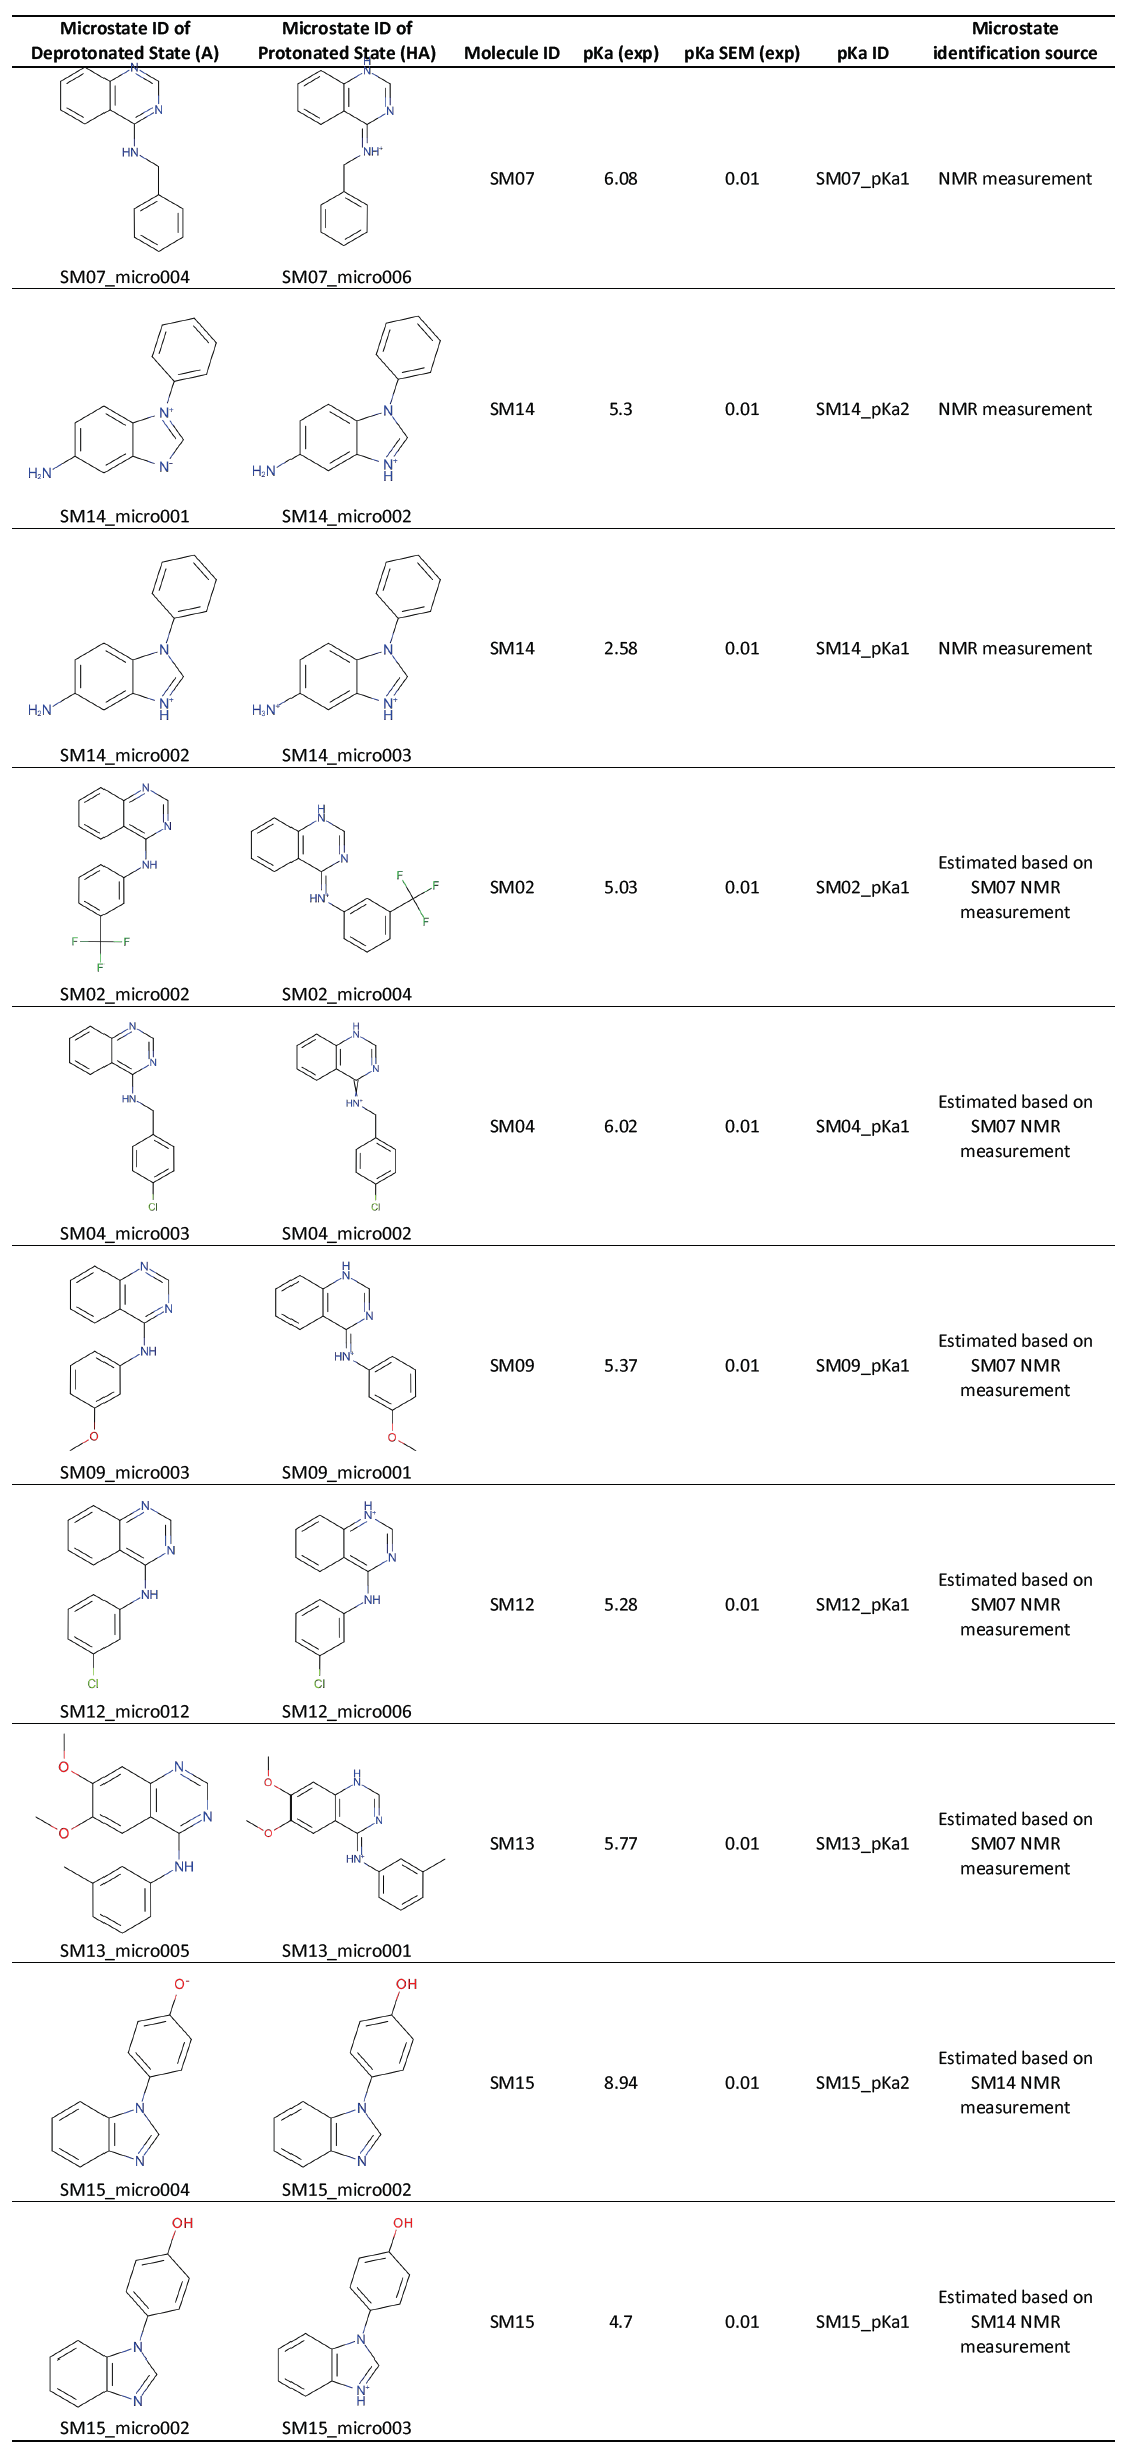
\includegraphics[width=0.5\linewidth]{figures/experimental-microstates-of-8mol-based-on-NMR.png}
\caption{ {\bf Dominant microstates of 8 molecules were determined based on NMR measurements.}
Dominant microstate sequence of 6 analogues were determined taking SM07 and SM14 as reference. 
Matched experimental \pKa{} values were determined by spectrophotometric \pKa{} measurements~\citep{Isik:2018:J.Comput.AidedMol.Des.}. 
A CSV version of this table can be found in \textit{SAMPL6-supplementary-documents.tar.gz}.
}
\label{fig:experimental-microstate-IDs-SI-table}
\end{figure}


\begin{figure}
\centering
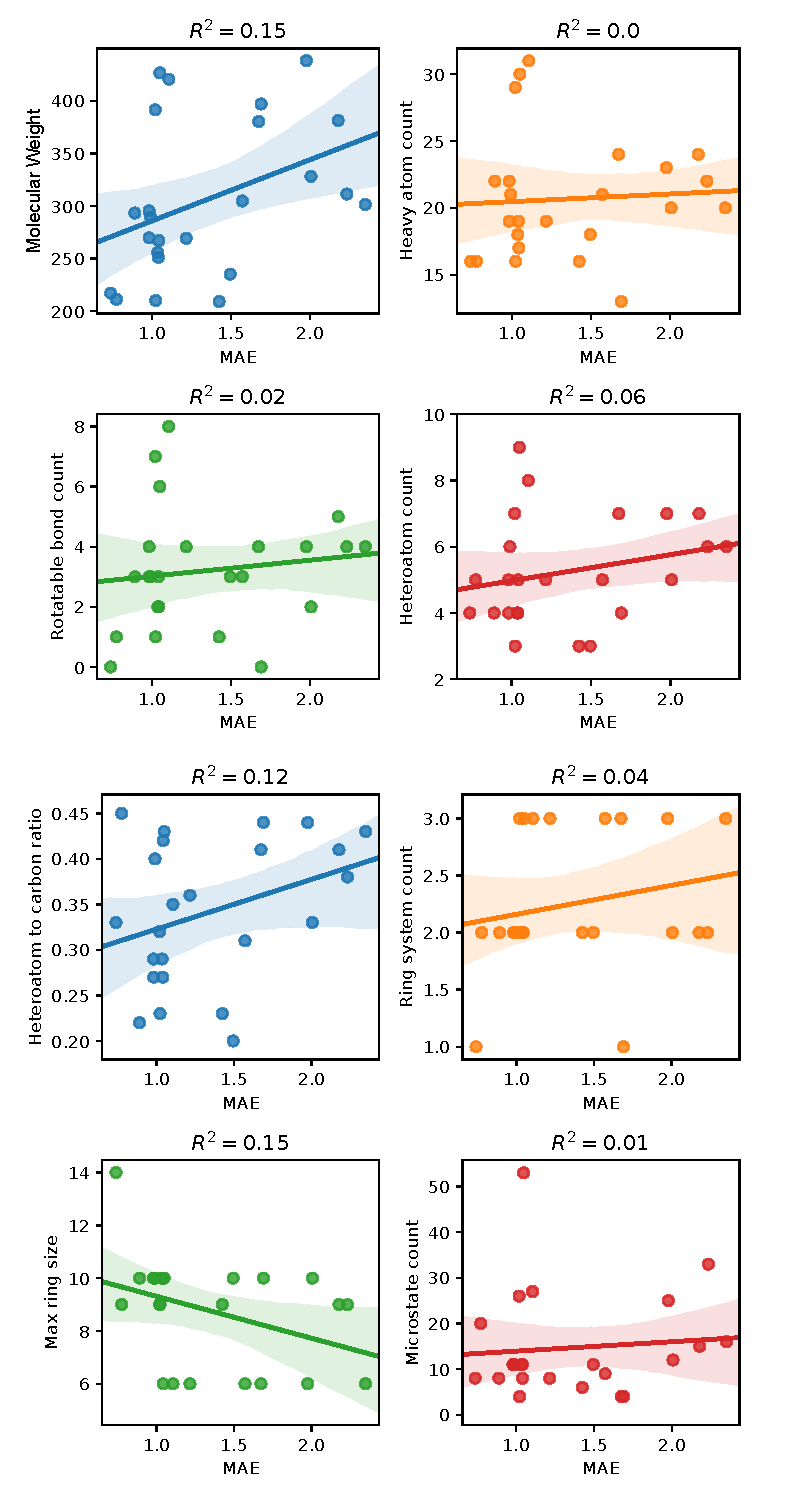
\includegraphics[width=0.5\linewidth]{figures/molecular_properties_vs_MAE_correlation_fig.pdf}
\caption{ {\bf MAE of macroscopic \pKa{} predictions of each molecule did not show any significant correlation with any molecular descriptor.} 
Plots show regression lines, 95\% confidence intervals of the regression lines, and R\textsubscript{2}. 
The following molecular descriptors were calculated using OpenEye OEMolProp Toolkit~\citep{oemolprop_openeye_2017}: molecular weight, non-terminal rotatable bond count, heteroatom to carbon ratio, maximum ring size, heavy atom count, heteroatom count, ring system count. 
Microstate count is based on the enumerated microstates for each compounds including additional microstates requested by participants.
}
\label{fig:molecular_properties_vs_MAE_correlation}
\end{figure}


\begin{figure}
\centering
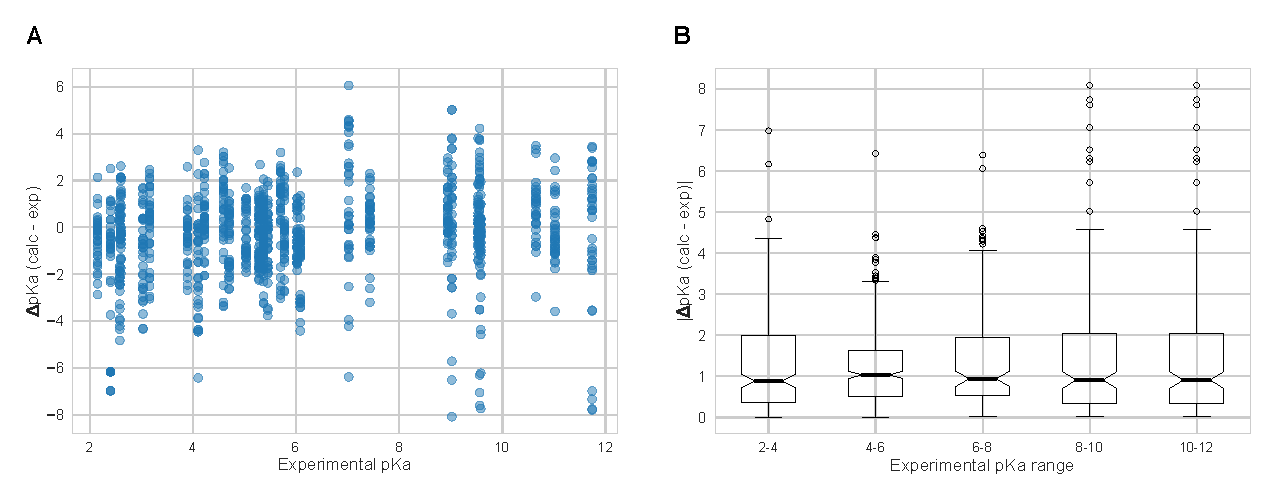
\includegraphics[width=1.0\linewidth]{figures/typeIII_error_vs_exp_pKa.pdf}
\caption{ {\bf The value of macroscopic \pKa{}s was not a factor affecting prediction error seen in SAMPL6 Challenge according to the analysis with Hungarian matching.} 
There was not clear trend between \pKa{} prediction error and the true \pKa{} error. 
Very high and very low \pKa{} values have similar inaccuracy compared to \pKa{} values close to 7.
{\bf A} Scatter plot of macroscopic \pKa{} prediction error calculated with Hungarian matching vs.\ experimental \pKa{} value {\bf B} Box plot of absolute error of macroscopic \pKa{} predictions binned into 2 \pKa{} unit intervals of experimental \pKa{}.
}
\label{fig:macroscopic-pKa-error-vs-pKa-value}
\end{figure}


\begin{figure}
\centering
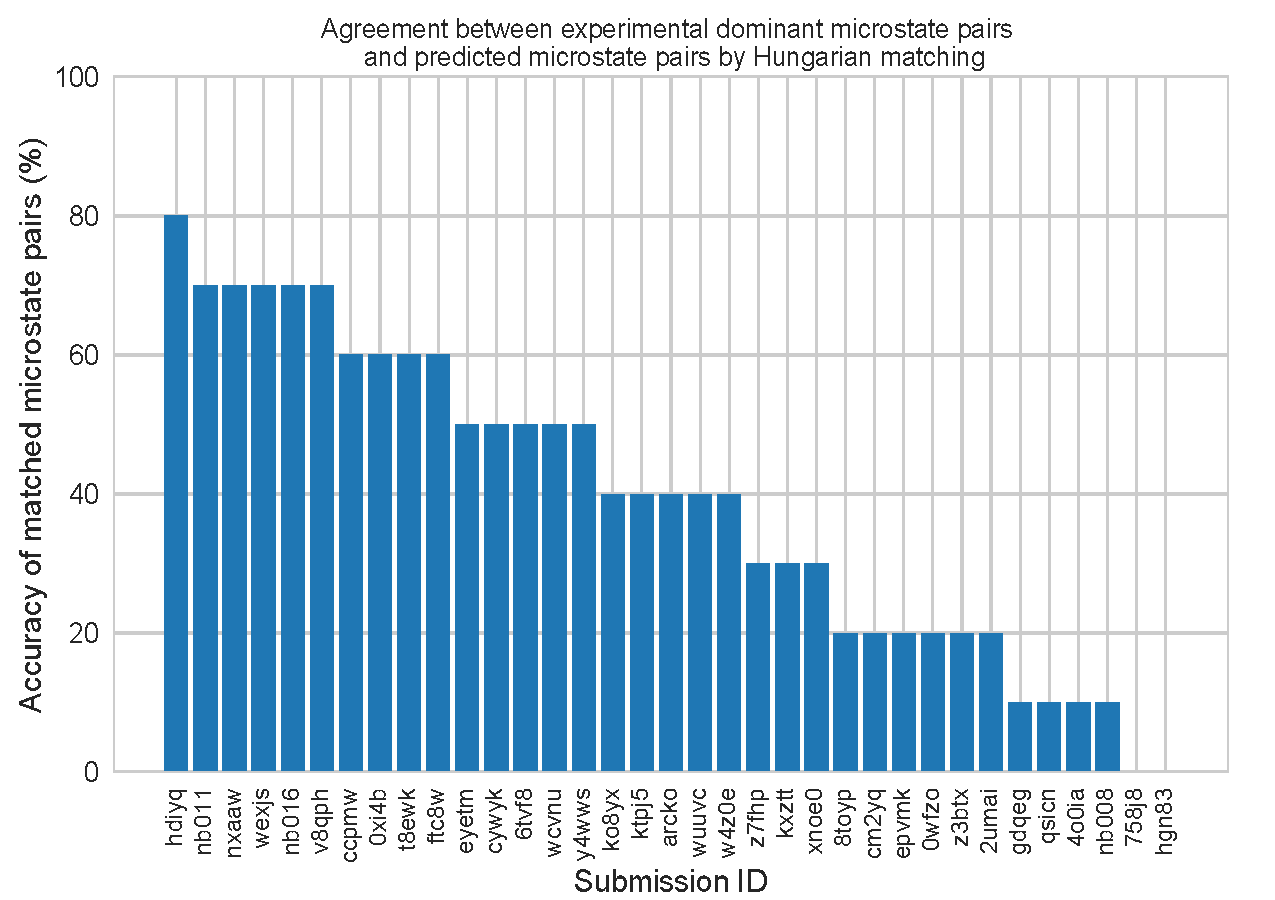
\includegraphics[width=0.75\linewidth]{figures/TypeI_Hungarian_match_microstate_pair_accuracy.pdf}
\caption{ {\bf There was low agreement between experimental dominant microstate pairs and the predicted microstate pairs selected by Hungarian algorithm for microscopic \pKa{} predictions.} 
This analysis could only be performed for 8 molecules with NMR data. 
Hungarian matching algorithm which matches predicted and experimental values considering only the closeness of the numerical value of \pKa{} and it often leads to predicted \pKa{} matches that described a different microstates pair than the experimentally observed dominant microstates.
}
\label{fig:microstate-pairs-with-Hungarian-match-vs-experiments}
\end{figure}



\end{document}
